%
% Template Laporan Tugas Akhir Jurusan Informatika Unsyiah 
%
% @author Abdul Hafidh
% @version 1.1
% @since 08.09.2023
%
% Template ini telah disesuaikan dengan aturan penulisan tugas akhir yang terdapat pada dokumen Panduan Tugas Akhir FMIPA Unsyiah tahun 2016.
%


% karena jifhasiltheme.cls ada di folder lib, maka kita harus menambahkan path lib/ ke dalam path pencarian file
\makeatletter
\def\input@path{{lib/}}
\makeatother
% Template pembuatan naskah tugas akhir.
\documentclass[dvipsnames]{jifhasiltheme-final}

\tolerance=1
\emergencystretch=\maxdimen
\hyphenpenalty=10000
\hbadness=10000

%\usepackage[a4paper,left=14cm,right=3cm,top=3cm,bottom=5cm]{geometry}
%karena file hype.indonesia.tex ada di folder language, maka kita harus menambahkan path language/ ke dalam path pencarian file
\makeatletter
\def\input@path{{language/}}
\makeatother
% Daftar pemenggalan suku kata dan istilah dalam LaTeX
%
% Hyphenation untuk Indonesia 
%
% @author  Andreas Febrian
% @version 1.00
% 
% Tambahkan cara pemenggalan kata-kata yang salah dipenggal secara otomatis 
% oleh LaTeX. Jika kata tersebut dapat dipenggal dengan benar, maka tidak 
% perlu ditambahkan dalam berkas ini. Tanda pemenggalan kata menggunakan 
% tanda '-'; contoh:
% menarik
%   --> pemenggalan: me-na-rik
%

\hyphenation{
    % alphabhet A
    a-na-li-sa a-tur 
    a-pli-ka-si 
    android
    % alphabhet B
    ba-ngun-an 
    be-be-ra-pa 
    ber-ge-rak
    ber-ke-lan-jut-an 
    ber-pe-nga-ruh 
    % alphabhet C
    ca-ri
    % alphabhet D
    di-sim-pan di-pim-pin de-ngan da-e-rah di-ba-ngun da-pat di-nya-ta-kan 
    di-sim-bol-kan di-pi-lih di-li-hat de-fi-ni-si
    % alphabhet E
    e-ner-gi eks-klu-sif
    % alphabhet F
    fa-si-li-tas
    foot-print
    % alphabhet G
    ga-bung-an ge-rak
    % alphabhet H
    ha-lang-an
    % alphabhet I
    % alphabhet J
    % alphabhet K
    ke-hi-lang-an
    ku-ning 
    kua-li-tas ka-me-ra ke-mung-kin-an ke-se-pa-ham-an
    % alphabhet L
    ling-kung-an
    % alphabhet M
    me-neng-ah
    meng-a-tas-i me-mung-kin-kan me-nge-na-i me-ngi-rim-kan 
    meng-u-bah meng-a-dap-ta-si me-nya-ta-kan mo-di-fi-ka-si
    meng-a-tur
    mem-pro-mo-si-kan
    me-la-ku-kan
    meng-i-den-ti-fi-ka-si-kan
    % alphabhet N
    nya-ta non-eks-klu-sif
    % alphabhet O
    % alphabhet P
	pe-nye-rap-an 
	pe-ngon-trol
    pe-mo-del-an
    pe-ran  pe-ran-an-nya
    pem-ba-ngun-an pre-si-den pe-me-rin-tah prio-ri-tas peng-am-bil-an 
    peng-ga-bung-an pe-nga-was-an pe-ngem-bang-an 
    pe-nga-ruh pa-ra-lel-is-me per-hi-tung-an per-ma-sa-lah-an 
    pen-ca-ri-an peng-struk-tur-an
    pe-ran-ca-ngan
    plat-form
    patch
    % alphabhet Q
    % alphabhet R
    ran-cang-an
    % alphabhet S
    si-mu-la-si sa-ngat
    smart-phone
    % alphabhet T
    te-ngah
    ter-da-pat
    % alphabhet U
    % alphabhet V
    % alphabhet W
    % alphabhet X
    % alphabhet Y
    % alphabhet Z
    % special
}

% Untuk prefiks pada daftar gambar dan tabel
\usepackage[titles]{tocloft}

\usepackage{etoolbox}% http://ctan.org/pkg/etoolbox
\makeatletter
% \patchcmd{<cmd>}{<search>}{<replace>}{<succes>}{<failure>}
\patchcmd{\@chapter}{\addtocontents{lof}{\protect\addvspace{10\p@}}}{}{}{}% LoF
\patchcmd{\@chapter}{\addtocontents{lot}{\protect\addvspace{10\p@}}}{}{}{}% LoT
\makeatother

\usepackage[justification=centering]{caption}% or e.g. [format=hang]

% Ini tambahan dari budi
\newcommand*{\enableboldchapterintoc}{%
  \addtocontents{toc}{\string\renewcommand{\protect\cftchapfont}{\protect\normalfont\protect\bfseries}}
  \addtocontents{toc}{\string\renewcommand{\protect\cftchappagefont}{\protect\normalfont\protect}}
  \addtocontents{toc}{\protect\setlength{\cftbeforechapskip}{12pt}}
}
\newcommand*{\disableboldchapterintoc}{%
  \addtocontents{toc}{\string\renewcommand{\protect\cftchappagefont}{\protect\normalfont}}
  \addtocontents{toc}{\string\renewcommand{\protect\cftchapfont}{\protect\normalfont}}
  \addtocontents{toc}{\protect\setlength{\cftbeforechapskip}{0pt}}
}
% Ini tambahan dari budi

\renewcommand{\cftdotsep}{0.5}
\renewcommand{\cftchapleader}{\cftdotfill{\cftdotsep}}
%\renewcommand{\cftpartleader}{\cftdotfill{\cftdotsep}}

\renewcommand\cftfigpresnum{Gambar\  }
\renewcommand\cfttabpresnum{Tabel\   }

\newcommand{\listappendicesname}{DAFTAR LAMPIRAN}
\newlistof{appendices}{apc}{\listappendicesname}
\newcommand{\appendices}[1]{\addcontentsline{apc}{appendices}{#1}}
\newcommand{\newappendix}[1]{\section*{#1}\appendices{#1}}

% Untuk hyperlink dan table of content
\usepackage[hidelinks]{hyperref}
\renewcommand\UrlFont{\rmfamily\itshape} %it's me!
\newlength{\mylenf}
\settowidth{\mylenf}{\cftfigpresnum}
\setlength{\cftfignumwidth}{\dimexpr\mylenf+2em}
\setlength{\cfttabnumwidth}{\dimexpr\mylenf+2em}

% Agar ada tulisan BAB pada TOC
\renewcommand\cftchappresnum{BAB } 
  \cftsetindents{chapter}{0em}{4.5em} %indenting bab
  \cftsetindents{section}{4.5em}{2em}
  \cftsetindents{subsection}{6.5em}{3em}
 
% Agar di TOC setiap angka bab/subbab diakhiri titik

\renewcommand{\cftsecaftersnum}{.}
\renewcommand{\cftsubsecaftersnum}{.}

\addtocontents{toc}{~\hfill \textit{Halaman}\par} % Menambahkan kata "Halaman" di sebelah kanan daftar isi

% Membuat juga kata "halaman" di daftar gambar dan daftar tabel
\addtocontents{lof}{~\hfill \textit{Halaman}\par}
\addtocontents{lot}{~\hfill \textit{Halaman}\par}

% Membuat juga kata "halaman" di daftar lampiran
\addtocontents{apc}{~\hfill \textit{Halaman}\par}

% Agar setiap angka bab/subbab diakhiri titik
\usepackage{titlesec}
\titlelabel{\thetitle.\quad}

% Agar disetiap caption table dan gambar diakhiri titik
\usepackage[labelsep=period]{caption}

% Untuk Bold Face pada Keterangan Gambar
\usepackage[labelfont=bf]{caption}

% Untuk caption dan subcaption
\usepackage{caption}
\usepackage{subcaption}


% Agar bisa menggunakan warna LaTeX
\usepackage{color} %it's me!

% Agar table yang panjang bisa cut ke next page    %byRennyAdr
\usepackage{longtable}

% Untuk page landscape        %byRennyAdr
\usepackage{pdflscape}
\usepackage{lscape}

% Agar bisa bikin code snippet
\usepackage{listings, lstautogobble} %it's me!

\usepackage{adjustbox}

% untuk shadow gambar     %tomy
\usepackage{fancybox, graphicx}

% untuk cite url
\usepackage{url}
\usepackage{microtype} % untuk mengatur spasi pada paragraf

\usepackage{siunitx}

\usepackage{xcolor}
\usepackage{multirow}
\usepackage[normalem]{ulem}
\useunder{\uline}{\ul}{}

\usepackage{array}
\newcolumntype{P}[1]{>{\centering\arraybackslash}p{#1}}
\newcolumntype{M}[1]{>{\centering\arraybackslash}m{#1}}


\makeatletter
\def\input@path{{include/}}
\makeatother
% Sampul Depan
%-----------------------------------------------------------------
% Sampul Depan
%-----------------------------------------------------------------
\judulcover{Perbandingan Kinerja Arsitektur VGG19-LSTM dan BLIP dalam \textit{Visual Question Answering} (VQA) pada Citra Medis}

\judul{Perbandingan Kinerja Arsitektur VGG19-LSTM dan BLIP dalam \textit{Visual Question Answering} (VQA) pada Citra Medis}

\judulinggris{\textit{PERFORMANCE COMPARISON OF VGG19-LSTM AND BLIP ARCHITECTURES IN VISUAL QUESTION ANSWERING (VQA) ON MEDICAL IMAGES}}

% nama lengkap
\fullname{Abdul Hafidh}

% NPM (Nomor Pokok Mahasiswa)
\idnum{2008107010056}

\degree{Sarjana Komputer}

\yearsubmit{Juni, 2024}

\program{Informatika}

\dept{Informatika}

% Pembimbing Pertama
\firstsupervisor{Alim Misbullah, S.Si., M.S.}
\firstnip{198806032019031011}

% Pembimbing Kedua
\secondsupervisor{Laina Farsiah, S.Si., M.S.}
\secondnip{198902032022032004}

% Ketua Jurusan
\kajur{Dr. Nizamuddin, M.Info.Sc.}
\kajurnip{198008312009122003}

% Dekan Fakultas
\dekan{Prof. Dr. Taufik Fuadi Abidin, S.Si., M.Tech}
\dekannip{197010081994031002}
% Dekan Fakultas
%\dekan{Dr. Teuku Mohamad Iqbalsyah, S.Si., M.Sc.}
%\dekannip{197110101997031003}

%kaprodi
\kaprodi{Alim Misbullah, S.Si., M.S.}
\kaprodinip{198806032019031011}

% tangal lulus proposal, seminar hasil atau sidang
\approvaldate{Kamis, 27 Juni 2024}

%-----------------------------------------------------------------
% End of Sampul Depan
%-----------------------------------------------------------------


% Awal dokumen
\usepackage{fancyhdr}
\usepackage{rotating}
% Untuk prefiks pada Daftar Program   
% byRennyAdr
\makeatletter
\begingroup\let\newcounter\@gobble\let\setcounter\@gobbletwo
\globaldefs\@ne \let\c@loldepth\@ne
\newlistof{listings}{lol}{\lstlistlistingname}
\endgroup
\let\l@lstlisting\l@listings
\AtBeginDocument{\addtocontents{lol}{\protect\addvspace{10\p@}}}
\makeatother
\renewcommand{\lstlistoflistings}{\listoflistings}
\renewcommand\cftlistingspresnum{Program~}
\cftsetindents{listings}{1.5em}{7em}

%tab didaftar pustaka -Indah
\setlength{\bibhang}{30pt}

%split rumus -Indah
\usepackage{amsmath}
\usepackage{pdfpages}

% \usepackage{multirow}
\usepackage[table,xcdraw]{xcolor}
\usepackage{colortbl}
% Beamer presentation requires  instead of \usepackage[table,xcdraw]{xcolor}
% \usepackage{longtable}

\begin{document}
\fancyhf{} 
\fancyfoot[C]{\thepage}



\cover

\approvalpage
%\includepdf[pages=-]{tanda-tangan/ttd-pengesahan-signed.pdf}

\bplagiasi % Note: \preface JANGAN DIHAPUS!

\noindent
Saya yang bertanda tangan di bawah ini,

\vspace{-0.1cm}

\begin{table}[H]
\begin{tabular}{M{0.6cm}ll}
	&Nama lengkap   		&: Abdul Hafidh \\
	&Tempat/tanggal lahir	&: Banda Aceh/29 Maret 2002 \\
	&NPM       			&: 2008107010056    \\
	&Program Studi   		&: Informatika \\
	&Fakultas 				&: MIPA \\
	&Judul Tugas Akhir      &: \begin{tabularx}{\linewidth}[t]{@{}X@{}}
		PERBANDINGAN KINERJA ARSITEKTUR VGG19-LSTM \\
		DAN BLIP DALAM \textit{VISUAL QUESTION ANSWERING} (VQA) \\ 
		PADA CITRA MEDIS
	   \end{tabularx}
	% &Judul Tugas Akhir      &: PENERAPAN \textit{VISUAL QUESTION ANSWERING} DALAM \\
	% &						&   MENAFSIRKAN CITRA MEDIS MENGGUNAKAN \\
	% &						&  \textit{DEEP LEARNING}
\end{tabular}
\end{table}

\vspace{0.2cm}
\noindent
Menyatakan dengan sesungguhnya bahwa Laporan Tugas Akhir saya dengan judul di atas adalah \textbf{hasil karya saya sendiri} bersama dosen pembimbing dan \textbf{bebas plagiasi}.

\vspace{1cm}
\noindent
Jika ternyata di kemudian hari terbukti bahwa Laporan Tugas Akhir merupakan hasil plagiasi, saya bersedia menerima sanksi yang berlaku di Universitas Syiah Kuala.

\vspace{1cm}


\begin{tabular}{p{7.5cm}l}
	&Banda Aceh, 27 Juni 2024\\
	&\\
	&\\
	&\multirow{1.5}{7.5cm}{\underline{Abdul Hafidh}} \\ 
	&NPM. 2008107010056 \\
\end{tabular}
%\includepdf[pages=-]{tanda-tangan/bebas-plagiasi-signed.pdf}
\spernyataan % Note: \preface JANGAN DIHAPUS!

\noindent
Yang bertanda tangan di bawah ini,
\vspace{-0.1cm}
\begin{table}[H]
{\renewcommand{\arraystretch}{0.7}
\begin{tabular}{M{0.6cm}lll}
	&1. 	& Nama   		&: Abdul Hafidh \\
	&	& NPM       			&: 2008107010056   \\
	&	& Jurusan/Prodi   		&: Informatika \\
	&	& Status 				&: Mahasiswa \\  
	&2. 	& Nama  		&: Alim Misbullah, S.Si., M.S. \\
	&	& NIP       			&: 198806032019031011    \\
	&	& Jurusan/Prodi   		&: Informatika \\
	&	& Status 				&: Pembimbing I \\  
	&3. 	& Nama  		&: Laina Farsiah, S.Si., M.S. \\
	&	& NIP       			&: 198902032022032004  \\
	&	& Jurusan/Prodi   		&: Informatika \\
	&	& Status 				&: Pembimbing II   
\end{tabular}
}
\end{table}
\vspace{-0.4cm}
\noindent
Dengan ini menyatakan hasil penelitian Tugas Akhir yang berjudul \textbf{PERBANDINGAN KINERJA ARSITEKTUR VGG19-LSTM DAN BLIP dalam \textit{Visual Question Answering} (VQA) PADA CITRA MEDIS} tidak dipublikasikan secara \textit{full-text} di sistem ETD (\textit{Electronic Theses and Dissertations}) Universitas Syiah Kuala hingga batas waktu 5 tahun dari tanggal kelulusan.

\vspace{0.4cm}
\noindent
Demikian surat pernyataan ini dibuat dengan sebenarnya untuk dapat dipergunakan seperlunya.

\vspace{0.4cm}
{\renewcommand{\arraystretch}{0.8}
\centering
\begin{tabular}{lll}
	&Darussalam, 8 Juli 2024		& \\
	&Yang membuat pernyataan,			& \\
	&&\\
	Pembimbing I,							&Pembimbing II,							&Mahasiswa,\\
	&&\\
	&&\\
	&&\\
	\underline{Alim Misbullah, S.Si., M.S.}	&\underline{Laina Farsiah, S.Si., M.S.} &\underline{Abdul Hafidh}\\
	NIP. 198806032019031011				&NIP. 198902032022032004				&NPM. 2008107010056\\
	&&\\
	&Mengetahui:\\			&
\end{tabular}
}
{\renewcommand{\arraystretch}{0.8}
\begin{tabular}{lll}
	Koordinator Program Studi Informatika	&\qquad\qquad  &Koordinator TA,\\
	Universitas Syiah Kuala,&\quad\quad  &\\
	&&\\
	&&\\
	&&\\
	\underline{Alim Misbullah, S.Si., M.S.}	&\quad\quad  &\underline{Alim Misbullah, S.Si., M.S.}\\
	NIP. 198806032019031011						&\quad\quad  &NIP. 198806032019031011				
\end{tabular}
}
%\includepdf[pages=-]{tanda-tangan/ttd-pernyataan-signed.pdf}

\begin{abstractind}

\textit{Visual Question Answering} (VQA) merupakan tugas untuk menjawab pertanyaan berdasarkan gambar. Dalam dunia medis, VQA dapat membantu ahli kesehatan untuk mendapatkan informasi dari citra medis. Namun, citra medis memiliki tantangan tersendiri, seperti variasi pertanyaan yang kompleks dan tingkat keabstrakan yang tinggi, sehingga memerlukan model VQA yang dapat menangani hal tersebut. Penelitian ini melakukan eksperimen dengan dua model, yaitu VGG19-LSTM dan BLIP, dengan \textit{dataset} PathVQA dan VQA-RAD. Model VGG19-LSTM menggabungkan \textit{Convolutional Neural Network} (CNN) dengan \textit{Long Short-Term Memory} (LSTM). BLIP adalah model terunifikasi untuk tugas \textit{vision-language} yang menggunakan \textit{Vision Transformers} (ViT) sebagai \textit{image encoder} dan \textit{transformer} sebagai \textit{text encoder}. Hasil eksperimen menunjukkan keunggulan model BLIP dalam kedua \textit{dataset}. BLIP yang dilatih dengan \textit{dataset} PathVQA dengan konfigurasi \textit{hyperparameter} 15 \textit{epochs}, \textit{batch size} 8, dan \textit{learning rate} $1 \times 10^{-5}$ setelah augmentasi pertanyaan mencapai akurasi 83,91\%, akurasi pertanyaan \textit{close-ended} 97,43\%, dan akurasi pertanyaan \textit{open-ended} 66,15\%. Model BLIP yang dilatih \textit{dataset} VQA-RAD dengan konfigurasi \textit{hyperparameter} 45 \textit{epochs}, \textit{batch size} 8, dan \textit{learning rate} $5 \times 10^{-5}$ setelah augmentasi pertanyaan mencapai akurasi 82,86\%, akurasi pertanyaan \textit{close-ended} 87,85\%, dan akurasi pertanyaan \textit{open-ended} 76,82\%. Pada tahap inferensi, model BLIP yang dikuantisasi menunjukkan performa yang lebih baik dibandingkan tanpa kuantisasi. Sebelum dilakukan kuantisasi, ukuran model BLIP adalah 1467,73 MB dengan waktu inferensi 0,24 detik pada \textit{dataset} PathVQA, dan 1467,73 MB dengan waktu inferensi 0,21 detik pada \textit{dataset} VQA-RAD. Setelah dilakukan kuantisasi, ukuran model BLIP menjadi 508,21 MB dengan waktu inferensi 0,20 detik pada \textit{dataset} PathVQA, dan 508,20 MB dengan waktu inferensi 0,17 detik pada \textit{dataset} VQA-RAD.




\bigskip
\noindent
\textbf{Kata kunci :} \textit{Visual Question Answering}, \textit{Convolutional Neural Network}, \textit{Long Short-Term Memory}, \textit{Transformer} VGG19-LSTM, BLIP, Citra Medis
\end{abstractind} %berikan comment jika proposal

\begin{abstracteng}

\textit{Visual Question Answering (VQA) is a task to answer questions based on images. In the medical world, VQA can help health experts to get information from medical images. However, medical images have their own challenges such as complex question variations and high levels of abstraction. Thus, it requires a VQA model that can handle these challenges. This research conducts experiments with two models, VGG19-LSTM and BLIP with PathVQA and VQA-RAD datasets. The VGG19-LSTM model combines Convolutional Neural Network (CNN) with Long Short-Term Memory (LSTM). BLIP is a unified model for vision-language tasks that uses Vision Transformers (ViT) as image encoders and transformers as text encoders. The experimental results show the superiority of the BLIP model in both datasets. BLIP trained with the PathVQA dataset with hyperparameter configuration of 15 epochs, batch size 8, and learning rate $1 \times 10^{-5}$ after question augmentation achieves an accuracy of 83.91\%, close-ended question accuracy of 97.43\%, and open-ended question accuracy of 66.15\%. After that, the BLIP model trained with the VQA-RAD dataset with hyperparameter configuration of 45 epochs, batch size 8, and learning rate $5 \times 10^{-5}$ after question augmentation achieves an accuracy of 82.86\%, close-ended question accuracy of 87.85\%, and open-ended question accuracy of 76.82\%. In the inference stage, the quantized BLIP model shows better performance than without quantization. Before quantization, the size of the BLIP model is 1467.73 MB with an inference time of 0.24 seconds on the PathVQA dataset, and 1467.73 MB with an inference time of 0.21 seconds on the VQA-RAD dataset. After quantization, the size of the BLIP model becomes 508.21 MB with an inference time of 0.20 seconds on the PathVQA dataset, and 508.20 MB with an inference time of 0.17 seconds on the VQA-RAD dataset.}

\bigskip
\noindent
\textit{\textbf{Keywords :}} \textit{Visual Question Answering}, \textit{Convolutional Neural Network}, \textit{Long Short-Term Memory}, \textit{Transformer} VGG19-LSTM, BLIP, \textit{Medical Image}
\end{abstracteng} %berikan comment jika proposal
%-----------------------------------------------------------------
% Disini kata pengantar
%-----------------------------------------------------------------
\preface % Note: \preface JANGAN DIHAPUS!

Segala puji dan syukur kehadiran Allah SWT yang telah melimpahkan rahmat dan hidayah-Nya kepada kita semua, sehingga penulis dapat menyelesaikan penulisan tugas akhir yang berjudul \textbf{“Perbandingan Kinerja Arsitektur VGG19-LSTM dan BLIP dalam \textit{Visual Question Answering} (VQA) pada Citra Medis”} yang telah dapat diselesaikan sesuai rencana. Penulis banyak mendapatkan berbagai pengarahan, bimbingan, dan bantuan dari berbagai pihak. Oleh karena itu, melalui tulisan ini penulis mengucapkan rasa terima kasih kepada:

\begin{enumerate}
	\item Dewi Ratna Sari, SE.MM, dan Fadhli, SE.Ak, sebagai kedua orang tua penulis, senantiasa memberikan dukungan penuh terhadap aktivitas dan kegiatan yang dilakukan penulis, baik secara moral maupun material, serta menjadi motivasi terbesar bagi penulis untuk menyelesaikan tugas akhir ini.
    \item Prof. Dr. Taufik Fuadi Abidin, S.Si., M.Tech, sebagai Dekan Fakultas MIPA Universitas Syiah Kuala.
    \item Dr. Nizamuddin, M.Info.Sc., sebagai Ketua Jurusan Informatika Fakultas MIPA Universitas Syiah Kuala.
    \item Bapak Alim Misbullah, S.Si., M.S., selaku Dosen Pembimbing I dan Ketua Program Studi Informatika, telah memberikan bimbingan dan arahan yang berharga kepada penulis, membantu penulis dalam menyelesaikan Tugas Akhir ini.
    \item Ibu Laina Farsiah, S.Si., M.S., selaku Dosen Pembimbing II, memberikan bimbingan dan arahan yang sangat dibutuhkan oleh penulis, yang akhirnya membantu penulis menyelesaikan tugas akhir ini.
    \item Ibu Sri Azizah Nazhifah, S.Kom., M.Sc., selaku dosen pembahas, telah membantu penulis dan kawan-kawan untuk mempersiapkan ruang lingkup tugas akhir, serta memberikan arahan yang diperlukan.
    \item Bapak dr. Muhammad Ansari Adista, M.Pd.Ked., Sp.N., selaku dosen pembahas yang telah memberikan masukan dan saran yang sangat berharga bagi penulis dalam menyelesaikan tugas akhir ini.
    \item Ibu Dalila Husna Yunardi, B.Sc., M.Sc., selaku dosen wali, memberikan \textit{support} dan pedoman yang diperlukan selama penulis menempuh pendidikan.
    \item Muhhamad Razan Fawwaz, Amar Suhendra, Khairul Umam Albi, Muhhamad Rudy Hidayat, Muhhamad Raja Furqan, Teuku Nabil Muhhamad Dhuha, Yoan Rifqi Candra, dan Haris Daffa, telah menemani dan memberi dukungan kepada penulis selama empat tahun perkuliahan di jurusan Informaika USK.
	\item Anas Naufal Al-Kiram, Muhhamad Hanif, Daffa Mudhaffar, Muhhamad Ikhsan Fikri, dan Teuku Muhhamad Roy Adrian, teman yang selalu mengingatkan, dan membantu penulis untuk selalu berusaha dalam menyelesaikan tugas akhir di semester 8.
    \item Sahabat dan teman-teman seperjuangan dari Jurusan Informatika USK 2020 lainnya, telah memberikan dukungan moral yang luar biasa selama penulis menempuh pendidikan di jurusan Informatika USK.
    \item Seluruh Dosen dan Staf di Jurusan Informatika Fakultas MIPA, atas ilmu dan bimbingan yang diberikan kepada penulis selama perkuliahan, menjadi bagian tak terpisahkan dalam proses pembelajaran penulis.
\end{enumerate}

%\vspace{1.5cm}

Penulis mengakui adanya kekurangan dalam tulisan ini, baik dari aspek materi, metode, maupun bahasa yang digunakan. Oleh karena itu, penulis mengundang kritik dan saran yang konstruktif dari para pembaca untuk meningkatkan kualitas Tugas Akhir ini. Penulis berharap bahwa tulisan ini dapat memberikan manfaat bagi banyak orang dan berkontribusi pada kemajuan ilmu pengetahuan.

\vspace{1cm}


% \begin{tabular}{p{7.5cm}l}
% 	&Banda Aceh, 14 Januari 2024\\
% 	&\\
% 	&\\
% 	&\underline{Abdul Hafidh} \\
% 	NPM. 2008107010056
	
% \end{tabular}


% \begin{tabular}{p{7.5cm}l}
% 	&Banda Aceh, 8 Juli 2024\\
% 	&\\
% 	&\\
% 	&\multirow{1.5}{7.5cm}{\underline{Abdul Hafidh}} \\ 
% 	&NPM. 2008107010056 \\
% \end{tabular}

%\includepdf[pages=-]{tanda-tangan/kata-pengantar-signed.pdf}

\titleformat{\section}{\normalfont\bfseries\uppercase}{\thesection}{1.7em}{} % Untuk membuat section menjadi kapital tapi daftar isi tetap non kapital

% Untuk subsection set saja jaraknya 1.5em (ga perlu buat kapital seperti section)
\titleformat{\subsection}{\normalfont\bfseries}{\thesubsection}{0.9em}{}




%-----------------------------------------------------------------
% TOC menggunakan single space
%-----------------------------------------------------------------

\addcontentsline{toc}{chapter}{Daftar Isi}
\begin{singlespace}
	\tableofcontents
\end{singlespace}
\listoftables
\addcontentsline{toc}{chapter}{Daftar Tabel}
\listoffigures
\addcontentsline{toc}{chapter}{Daftar Gambar}

% \renewcommand{\lstlistlistingname}{DAFTAR PROGRAM}
% \lstlistoflistings
% \addcontentsline{toc}{chapter}{Daftar Program}

\listofappendices
\addcontentsline{toc}{chapter}{Daftar Lampiran}

\enableboldchapterintoc
%-----------------------------------------------------------------
% Daftar Singkatan 
%-----------------------------------------------------------------
\include{daftar-singkatan}

% Caption untuk code snippet. it's me!
\renewcommand{\thelstlisting}{\arabic{chapter}.\arabic{lstlisting}}
\renewcommand*\lstlistingname{Program}

%-----------------------------------------------------------------
% Disini awal masukan untuk Bab
%-----------------------------------------------------------------
\begin{onehalfspace}

\fancyhf{} 
\fancyfoot[C]{\thepage}
\pagenumbering{arabic}

\captionsetup[figure]{labelfont={normalfont}, textfont={normalfont}} % Unbold caption gambar
\captionsetup[table]{labelfont={normalfont}, textfont={normalfont}} % Unbold caption tabel

\fancyhf{} 
\fancyfoot[R]{\thepage}

% \fancyhf{} 
% \fancyfoot[C]{\thepage}


\chapter{PENDAHULUAN}
% \thispagestyle{plain} % Halaman pertama bab menggunakan gaya plain


\section{Latar Belakang}

\par Citra medis, seperti \textit{Magnetic Resonance Imaging} (MRI), \textit{X-Ray}, \textit{Ultrasonography} (USG), \textit{Endoscopy}, \textit{Computed Tomography} (CT-Scan), \textit{Nuclear Medicine}, dan lain-lain, menjadi fokus penelitian utama dalam dunia medis \citep{kusuma2020penerapan}. Profesional medis menggunakan berbagai teknik untuk mendeteksi dan menganalisis penyakit pada pasien. Dua cabang ilmu yang berkaitan dengan diagnosa penyakit, yaitu patologi dan radiologi, memainkan peran krusial dalam memahami citra medis \citep{sorace2012integrating}. Meskipun demikian, kesalahan analisis citra medis oleh tenaga medis terkadang bisa saja terjadi karena sifat manusia yang rentan terhadap kesalahan \citep{mauli2018tanggung}. 


\par Ketika manusia melakukan pekerjaan yang repetitif, ini dapat menyebabkan kelelahan dan berkurangnya konsentrasi, sehingga meningkatkan kemungkinan kesalahan. Hal ini berbeda dengan \textit{Artificial Intelligence} (AI), AI tidak memiliki perasaan, sehingga AI akan tetap menghasilkan kualitas pekerjaan yang konsisten seiring berjalannya waktu \citep{fernando2019studi}. Pada bidang medis AI tidak diharapkan untuk menggantikan dokter manusia dalam skala besar. Sebaliknya, AI kemungkinan akan memberdayakan praktik kedokteran dengan meningkatkan upaya dokter dan mengatasi masalah seperti kelelahan dokter \citep{basu2020artificial}. Oleh sebab itu, dibutuhkan sebuah sistem yang dapat membantu tenaga medis dalam menjawab permasalahan yang terdapat pada citra medis. Salah satu solusi yang dapat digunakan adalah dengan membangun sistem \textit{Visual Question Answering} (VQA). Dalam konteks medis VQA dapat memberikan manfaat bagi dokter dan pasien yang mana dokter bisa memperoleh jawaban yang diperoleh dari sistem VQA sebagai bentuk dalam pengambilan keputusan. Sedangkan pasien bisa mengajukan pertanyaan ke sistem VQA dengan gambar medis yang ada pada dirinya untuk mengetahui kondisi kesehatanya \citep{aioz_mevf_miccai19}.

\par Sistem VQA medis ini juga dapat berperan sebagai asisten yang memiliki pengetahuan yang luas. Sebagai contoh, pendapat tambahan atau opini kedua dari sistem VQA dapat membantu tenaga medis dalam menjawab pertanyaan berdasarkan citra medis yang diberikan dan mengurangi potensi kesalahan dalam diagnosis pada saat bersamaan \citep{tschandl2020human}. Meskipun begitu, penelitian mengenai sistem VQA medis masih terbatas karena menghadapi beberapa tantangan khusus yang harus dihadapi, seperti keanekaragaman pertanyaan yang dapat diajukan, yang memerlukan pemahaman yang mendalam tentang citra medis dan pertanyaan untuk konteks medis, serta memiliki keterbatasan dalam interpretabilitas yakni kemampuan untuk menanyakan model tentang wilayah gambar yang spesifik \citep{lin2023medical}. Akan tetapi, dengan sering dilakukannya penelitian terkait \textit{medical visual question answering}, diharapkan dapat mengatasi tantangan yang ada, sehingga penelitian \textit{medical visual question answering} dapat berkembang dengan baik seiring berjalannya waktu.

\par Penelitian ini bertujuan untuk mengembangkan sebuah sistem VQA yang mampu memberikan jawaban terhadap pertanyaan yang diajukan berdasarkan citra medis. Sistem ini akan memanfaatkan dua \textit{dataset} yaitu PathVQA yang terkait dengan patologi, dan VQA-RAD yang fokus pada bidang radiologi. Dalam penelitian ini akan menggunakan pendekatan \textit{deep learning} yang memanfaatkan teknik \textit{transfer learning}. Teknik \textit{transfer learning} ini digunakan untuk memanfaatkan model yang sudah dilatih sebelumnya pada \textit{dataset} yang berbeda. Hasil dari penelitian ini diharapkan dapat memberikan gambaran mengenai sistem VQA untuk citra medis dengan \textit{deep learning} dan memberikan kontribusi terkait penelitian \textit{medical visual question answering}.

\section{Rumusan Masalah}
Berdasarkan latar belakang yang telah diuraikan, permasalahan dalam penelitian ini dapat dirumuskan sebagai berikut:
\begin{enumerate}

	\item{Bagaimana membangun model VQA menggunakan citra medis dengan menerapkan teknik \textit{transfer learning}?}

	\item{Bagaimana membandingkan performa model VQA pada arsitektur VGG19-LSTM dan BLIP untuk \textit{dataset} PathVQA dan VQA-RAD?}

    \item{Bagaimana menerapkan model VQA terbaik untuk menjawab pertanyaan berdasarkan citra medis?}

\end{enumerate}

\section{Tujuan Penelitian}
Adapun maksud dan tujuan dari penelitian ini adalah sebagai berikut:

\begin{enumerate}
	
	\item{Membangun model VQA menggunakan citra medis dengan menerapkan teknik \textit{transfer learning}.}

	\item{Membandingkan performa model VQA pada arsitektur VGG19-LSTM dan BLIP, dengan \textit{dataset} PathVQA dan VQA-RAD.}

	\item{Mengimplementasikan model VQA terbaik untuk menjawab pertanyaan berdasarkan citra medis.}

\end{enumerate}

\section{Manfaat Penelitian}
\par Manfaat yang diinginkan dari penelitian ini adalah untuk memberikan gambaran mengenai sistem VQA untuk citra medis dengan \textit{deep learning}. Selanjutnya, memberikan pengetahuan hasil implementasi dengan arsitektur VGG19-LSTM dan BLIP dalam mengembangkan sistem VQA pada citra medis. Lalu yang terakhir, memberikan kontribusi terkait penelitian \textit{medical visual question answering}. 

% \end{enumerate}




% Baris ini digunakan untuk membantu dalam melakukan sitasi
% Karena diapit dengan comment, maka baris ini akan diabaikan
% oleh compiler LaTeX.
\begin{comment}
\bibliography{daftar-pustaka}
\end{comment}

\fancyhf{} 
\fancyfoot[R]{\thepage}

%-------------------------------------------------------------------------------
%                            BAB II
%               TINJAUAN PUSTAKA DAN DASAR TEORI
%-------------------------------------------------------------------------------
%\fancyhf{}
% \fancyfoot[C]{\thepage}
\chapter{TINJAUAN KEPUSTAKAAN}
% \thispagestyle{plain} % Halaman pertama bab menggunakan gaya plain



% \par Untuk mendukung penelitian ini, maka dalam bab ini akan dikemukakan beberapa rumusan teori pendukung yang dikutip dari berbagai referensi baik dalam bentuk buku, artikel, maupun tulisan karya ilmiah lainnya termasuk hasil penelitian sebelumnya yang ada kaitannya dengan penelitian yang dilakukan.

% Mengatur format untuk bagian (section)


\section{Citra Medis}


\par Citra adalah gambaran dari suatu objek yang bisa kita lihat. Citra analog tidak bisa disimpan secara langsung dalam komputer. Oleh karena itu, kita perlu mengubah citra analog menjadi citra digital agar bisa diolah oleh komputer. Citra digital adalah citra yang bisa diolah menggunakan perangkat komputer. Alasan utama citra analog tidak bisa diolah oleh komputer adalah karena citra analog tidak memiliki konsep sampling dan kuantisasi. Konsep sampling adalah suatu metode yang mengubah citra analog menjadi \textit{grid} berbentuk M baris dan N kolom, sehingga citra menjadi lebih tersegmentasi. Semakin besar nilai M dan N, semakin halus citra digital yang dihasilkan. Sedangkan konsep kuantisasi adalah suatu metode yang mengubah intensitas dari citra analog menjadi intensitas diskrit. Baik sampling maupun kuantisasi memegang peranan penting dalam mengambil potongan citra menjadi bentuk M baris dan N kolom (proses sampling) serta menentukan nilai intensitas yang terdapat pada setiap titik tersebut (proses kuantisasi). Hasil akhir dari kedua konsep ini adalah citra yang memiliki resolusi sesuai dengan yang kita inginkan \citep{andono2018pengolahan}.

\par Dalam ilmu pengolahan citra, beragam jenis citra ada, dan salah satunya adalah citra \textit{Red Green Blue} (RGB), juga disebut sebagai citra \textit{true color}. Citra ini memiliki matriks data berukuran $m \times n \times 3$, yang menggambarkan warna merah, hijau, dan biru pada setiap piksel. Rentang nilai untuk setiap warna adalah antara 0 (nilai minimum) hingga 255 (nilai maksimum) dalam monitor komputer. Pada bagian ini, skala 0 hingga 255 dipilih berdasarkan representasi delapan digit dalam bilangan biner yang digunakan oleh komputer. Dengan demikian, lebih dari 16 juta warna dapat dihasilkan secara total. Penentuan warna pada setiap piksel didasarkan pada tingkat kecerahan merah, hijau, dan biru \citep{ardiansyah2013pengenalan}.

\par Di bidang kesehatan, pencitraan medis memegang peranan penting dalam berbagai bidang klinis seperti prosedur medis yang digunakan untuk deteksi dini, pemantauan, diagnosis, dan evaluasi pengobatan berbagai kondisi medis \citep{puttagunta2021medical}. Citra medis merujuk pada gambar dua dimensi yang menggambarkan struktur internal tubuh manusia, dimanfaatkan oleh profesional kesehatan untuk diagnosis penyakit. Pengolahan citra medis memiliki aplikasi luas, termasuk deteksi tumor atau kanker pada organ reproduksi wanita, identifikasi patologi pada organ-organ seperti paru-paru, hati, dan tulang, segmentasi struktur tulang dari jaringan otot, klasifikasi gigi, serta analisis gambar dari mikroskop. Berbagai teknologi digunakan dalam pencitraan medis ini, antara lain \textit{Magnetic Resonance Imaging} (MRI), \textit{X-Ray}, \textit{Ultrasonography} (USG), endoskopi, \textit{Computed Tomography} (CT-Scan), dan \textit{Nuclear Medicine} \citep{kusuma2018penerapan}. 

% Untuk memahami citra medis diperlukan bidang keilmuan yang mempelajari suatu asal usul penyakit yang disebut patologi \citep{cohnheim1889lectures}, dan bidang keilmuan yang mempelajari yang mempelajari cara mendiagnosa penyakit dengan menggunakan citra medis yang disebut radiologi \citep{wang2012machine}.

\section{\textit{Deep Learning}} 

\par \textit{Deep learning} adalah cabang ilmu \textit{machine learning} yang berbasis pada \textit{Artificial Neural Network} (ANN) sebagai pengembanganya. Metode dalam \textit{machine learning} biasanya hanya mengandalkan alat seperti \textit{Central Processing Unit} (CPU) dan \textit{Random Access Memory} (RAM) dalam menentukan kecepatan komputasi. Sedangkan metode \textit{deep learning} selain menggunakan CPU dan RAM, metode ini juga menggunakan \textit{Graphics Processing Unit} (GPU) sehingga proses komputasi data yang besar dapat dilakukan dengan cepat \citep{ilahiyah2018implementasi}.

\par \textit{Deep learning} memiliki pendekatan yang dapat dikategorikan seperti \textit{supervised learning}, \textit{unsupervised learning}, \textit{semi-supervised learning}, dan \textit{reinforcement learning} \citep{alom2019state}. Kategori pendekatan \textit{deep learning} dapat dilihat pada Gambar \ref{pendekatan-deeplearning}.

\begin{figure}[H]
    \centering
    {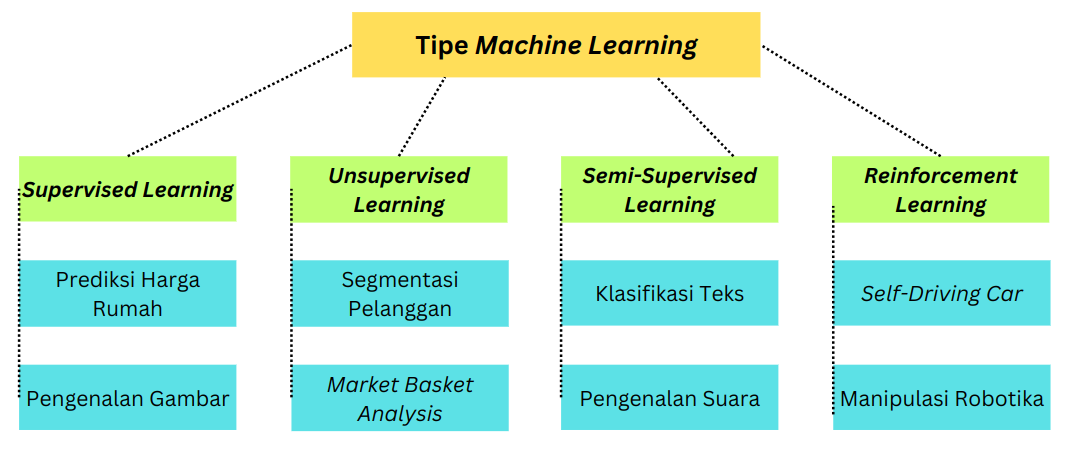
\includegraphics [width=\textwidth]{image/bab2/pendekatan-deep-learning.png}}
    \caption{Kategori pendekatan \textit{deep learning}}
    \label{pendekatan-deeplearning}
\end{figure}


\par Pendekatan ini melibatkan berbagai teknik dan algoritma untuk menyelesaikan berbagai jenis masalah. Dalam mengimplementasikan model \textit{deep learning}, beberapa \textit{hyperparameter} yang sangat penting untuk diperhatikan adalah \textit{learning rate}, \textit{batch size}, jumlah \textit{epochs}, dan arsitektur jaringan itu sendiri. \textit{Learning rate} adalah ukuran yang menentukan seberapa besar langkah yang diambil model saat memperbarui bobot selama pelatihan. \textit{Batch size} mengacu pada jumlah sampel data yang diproses sebelum memperbarui parameter model, sementara jumlah \textit{epochs} menunjukkan berapa kali seluruh \textit{dataset} akan dilalui selama pelatihan. Pemilihan \textit{hyperparameter} sering kali dilakukan dengan fleksibilitas berdasarkan eksperimen dan kebutuhan spesifik dari proyek yang sedang dikerjakan. Tidak ada aturan tetap mengenai nilai-nilai spesifik yang harus dipilih untuk \textit{hyperparameter}. Seorang peneliti dapat mencoba berbagai nilai untuk menemukan kombinasi yang optimal. Metode seperti \textit{grid search} menunjukkan bahwa nilai-nilai \textit{hyperparameter} dapat dipilih secara bebas dalam rentang yang telah ditentukan \citep{bergstra2012random}.


\par \textit{Grid search} adalah metode pencarian \textit{hyperparameter} yang melibatkan pencarian melalui ruang \textit{hyperparameter} dengan mencoba setiap kombinasi yang mungkin dari nilai \textit{hyperparameter} yang telah ditentukan sebelumnya. Dengan \textit{grid search}, seorang peneliti membuat sebuah \textit{grid} dari \textit{hyperparameter} yang berbeda dan mengevaluasi model dengan setiap kombinasi yang ada di \textit{grid} tersebut \citep{bergstra2012random}. Pendekatan ini memastikan bahwa semua kombinasi yang mungkin diuji, meskipun bisa sangat memakan waktu dan sumber daya.



\par Pada bidang medis \textit{deep learning} digunakan untuk memproses citra medis seperti X-rays, CT, scan MRI (\textit{Magnetic Resonance Imaging}) dan lain-lain untuk mendiagnosa kondisi kesehatan \citep{kelleher2019deep}.

\subsection{\textit{Artificial Neural Network}}

\par \textit{Artificial Neural Network} (ANN) atau jaringan saraf tiruan adalah jaringan saraf yang memproses informasi dengan cara yang mirip dengan otak manusia \citep{kristiyanti2023machine}. \textit{Neural network} terdiri dari elemen pemrosesan sederhana yang disebut \textit{node} yang saling terhubung, mirip dengan cara kerja neuron dalam otak manusia. Kemampuan untuk melakukan pemrosesan dalam jaringan ini disimpan dalam koneksi antara \textit{node}, yang biasanya disebut sebagai \textit{weight}. Nilai-nilai \textit{weight} ini diperoloeh melalui proses pembelajaran atau adaptasi yang berdasarkan pada pola data yang dipelajari oleh ANN \citep{gurney1997introduction}.

\subsection{Fungsi Aktivasi}


\par Fungsi aktivasi dalam konteks jaringan saraf dapat diibaratkan dengan cara tubuh manusia merespon rangsangan dari lingkungan. Ketika seseorang menerima rangsangan eksternal, tubuhnya secara otomatis meresponsnya. Sebagai contoh, ketika tangan kita digigit, tubuh kita akan merespons dengan menolak atau melepaskan gigitan tersebut. Respons tubuh ini akan semakin intens jika rangsangan yang diterima semakin kuat. Dalam konteks algoritma jaringan saraf, respons tubuh ini analoginya digantikan oleh nilai bobot dan tingkat aktivasi yang tinggi. Pada persamaan \ref{eq: neural network sebelum fungsi aktivasi} menunjukkan persamaan dari jaringan saraf sebelum menggunakan fungsi aktivasi.

% rumus neural network sebelum fungsi aktivasi

\begin{equation}
    % Rumus neural network sebelum fungsi aktivasi
    y = \sum_{i=1}^n x_i w_i + b
    \label{eq: neural network sebelum fungsi aktivasi}
\end{equation}

\begin{itemize}

    \item $y$ adalah nilai keluaran dari jaringan saraf.
    \item $x_i$ adalah nilai \textit{input} dari jaringan saraf.
    \item $w_i$ adalah bobot dari setiap nilai \textit{input}.
    \item $b$ adalah bias dari jaringan saraf.

\end{itemize}

\par Ketika menerapkan fungsi aktivasi pada persamaan \ref{eq: neural network sebelum fungsi aktivasi}, maka persamaan akan berubah menjadi seperti yang ditunjukkan pada persamaan \ref{rumus-fungsi-aktivasi}.

% rumus fungsi aktivasi

\begin{equation}
    % Rumus fungsi aktivasi
    z = \textit{Act}(\sum_{i=1}^n x_i w_i + b)
    \label{rumus-fungsi-aktivasi}
\end{equation}

\begin{itemize}
    \item $z$ adalah nilai keluaran dari jaringan saraf setelah menggunakan fungsi aktivasi.
    \item $Act$ adalah fungsi aktivasi.
    \item $x_i$ adalah nilai \textit{input} dari jaringan saraf.
    \item $w_i$ adalah bobot dari setiap nilai \textit{input}.
    \item $b$ adalah bias dari jaringan saraf.
\end{itemize}

\par Persamaan \ref{rumus-fungsi-aktivasi} ini menunjukkan bahwa nilai keluaran $z$ akan bergantung pada fungsi aktivasi terhadap nilai prediksi yang dihasilkan dari perkalian nilai \textit{input} dan bobot \citep{kristiyanti2023machine}. 

\par Fungsi aktivasi adalah komponen penting dalam jaringan saraf tiruan yang mengatur bagaimana nilai hasil penjumlahan terbobot dari \textit{input} data diubah menjadi \textit{output} yang dikeluarkan oleh neuron dalam jaringan saraf. Fungsi aktivasi ini digunakan untuk menentukan apakah suatu neuron akan meneruskan nilai kalkulasinya ke neuron berikutnya, berdasarkan suatu nilai ambang tertentu. Fungsi ini juga sering disebut sebagai fungsi transfer karena memiliki kemampuan untuk mengubah data yang dihasilkan dari hasil penjumlahan terbobot pada suatu lapisan, yang kemudian akan diteruskan ke lapisan selanjutnya. Fungsi aktivasi bisa berupa fungsi linear atau fungsi non-linear tergantung pada tugas yang ingin diselesaikan, dan fungsi aktivasi ini dapat digunakan dalam berbagai hal seperti pengenalan objek dan klasifikasi \citep{nwankpa2018activation}.

\par Fungsi aktivasi perlu memiliki sifat diskriminatif, yang merupakan aspek yang penting karena memungkinkan penggunaan proses propagasi balik kesalahan dalam pelatihan jaringan. Salah satu fungsi aktivasi yang umum digunakan dalam konteks CNN adalah fungsi ReLU (\textit{Rectified Linear Unit}). Fungsi ini merupakan fungsi aktivasi yang mengubah seluruh isi nilai \textit{input} menjadi angka positif \citep{alzubaidi2021review}. Persamaan fungsi aktivasi ini dapat dilihat pada persamaan \ref{eq:relu}.

\begin{equation}
    % Rumus fungsi aktivasi ReLU
    f(x)_\text{ReLU} = \max(0, x)
    \label{eq:relu}
\end{equation}

\par Salah satu fungsi aktivasi yang digunakan dalam berbagai model mutakhir seperti GPT-3, BERT, dan sebagian besar model Transformer lainya adalah \textit{Gaussian Error Linear Unit} (GELU). Fungsi ini merupakan fungsi aktivasi yang menimbang \textit{input} berdasarkan persentilnya, daripada mengelompokkan \textit{input} berdasarkan tandanya seperti ReLU. Oleh karena itu, GELU dapat dikatakan lebih mulus dibandingkan ReLU. Hal ini memungkinkan GELU untuk lebih mudah memperkirakan fungsi yang rumit daripada ReLU atau ELU \citep{hendrycks2016gaussian}. Persamaan fungsi aktivasi ini dapat dilihat pada persamaan \ref{eq:gelu}.

\begin{equation}
    % Rumus fungsi aktivasi GELU
    \operatorname{GELU}(x)=x P(X \leq x)=x \Phi(x)=x \cdot \frac{1}{2}[1+\operatorname{erf}(x / \sqrt{2})]
    \label{eq:gelu}
\end{equation}

\begin{itemize}

    \item{$x$ adalah nilai \textit{input} dari fungsi aktivasi.}

    \item{$\Phi$ adalah \textit{Cumulative Distribution Function} (CDF) dari $x$.}

    \item{$\operatorname{erf}$ adalah fungsi kesalahan dari $x$.}


\end{itemize}


\par Salah satu fungsi aktivasi yang dapat digunakan untuk mengklasifikasi lebih dari dua kelas adalah fungsi aktivasi \textit{softmax}. Persamaan \ref{eq:softmax} menunjukkan persamaan dari fungsi aktivasi \textit{softmax}.

\begin{equation}
    f_j(Z) = \frac{e^{z_j}}{\sum_k e^{z_k}}
    \label{eq:softmax}
\end{equation}

\par Pada persamaan \ref{eq:softmax}, Notasi $f_j$ menunjukkan hasil fungsi pada setiap elemen ke-j pada vektor keluaran kelas. Argumen $z$ merupakan hipotesis yang diberikan oleh model pelatihan agar dapat diklasifikasi oleh fungsi \textit{softmax} \citep{ilahiyah2018implementasi}. 



\subsection{Fungsi \textit{loss}}

\par Fungsi \textit{loss} adalah salah satu fungsi pada \textit{Artificial Neural Network} (ANN) untuk melakukan perhitungan nilai \textit{error} atau kesalahan dari hasil prediksi dari suatu \textit{output} ANN \citep{zhang2016neural}. 

\par Fungsi \textit{loss} yang menghukum kesalahan probabilitas \textit{false negative} daripada \textit{false positive} adalah \textit{categorical cross entropy} \citep{ho2019real}. Persamaan \ref{eq:categorical_cross_entropy} menunjukkan persamaan dari \textit{categorical cross-entropy}. 

\begin{equation}
    J_{cce} = -\frac{1}{M} \sum_{k=1}^{K} \sum_{m=1}^{M} y_{m}^{k} \log_{(\theta} (x_{m}, k)
    \label{eq:categorical_cross_entropy}
\end{equation}

% keterangan rumus categorical cross entropy

\begin{itemize}

    \item $M$ adalah jumlah sampel data yang digunakan untuk pelatihan.
    \item $K$ adalah jumlah kelas yang ada pada data.
    \item $y_{m}^{k}$ adalah nilai target dari sampel data ke-$m$ pada kelas ke-$k$.
    \item $x$ adalah \textit{input} untuk contoh pelatihan ke-$m$.
    \item $H_\theta$ adalah bobot model \textit{neural network} $\theta$.
\end{itemize}



    

\subsection{Fungsi Optimasi}

\par Fungsi optimasi atau \textit{optimization function} dapat diartikan sebagai suatu fungsi yang berperan sebagai \textit{black box}, dimana fungsi ini menerima kesalahan sebagai input dan menghasilkan nilai bobot yang optimal untuk suatu model ANN \citep{li2017learning}.

\par Salah satu dari fungsi optimasi yang dapat digunakan dalam pengembangan model \textit{deep learning} adalah Adam (\textit{Adaptive Moment Estimation}). Adam adalah teknik optimasi untuk \textit{gradient descent}. Metode ini sangat efisien saat bekerja dengan masalah yang melibatkan banyak data atau parameter. Algoritma ini membutuhkan memori yang lebih sedikit dan efisien. Secara intuitif, Adam merupakan gabungan antara algoritma \textit{stochastic gradient descent momentum} dan \textit{RMSProp}. Secara eksperimen Adam adalah teknik optimasi terbaik dengan \textit{training cost} yang rendah menurut \citep{kingma2014adam}. Gambar \ref{fig:adam} menunjukkan perbandingan teknik optimasi Adam dengan teknik optimasi lainnya.

\begin{figure}[H]
    \centering
    {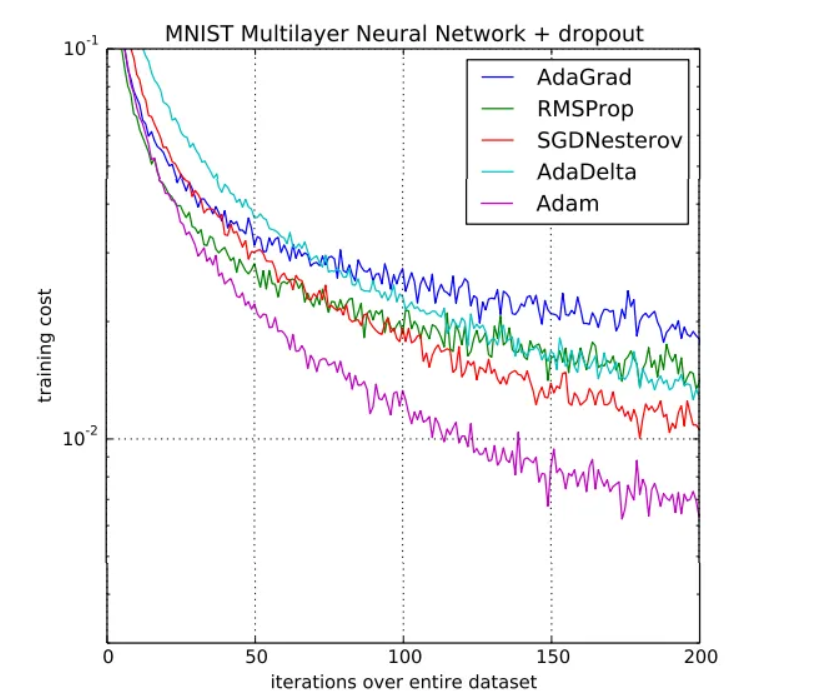
\includegraphics [width=\textwidth,height=8cm]{image/bab2/graf-optimisasi}}
    \caption{Perbandingan teknik optimasi Adam dengan teknik optimasi lainnya \citep{kingma2014adam}}
    \label{fig:adam}
\end{figure}


\section{\textit{Convolutional Neural Network}}

\par \textit{Convolutional Neural Network} (CNN) adalah turunan dari algoritma \textit{neural network} yang dikhususkan untuk memproses data yang berupa gambar. CNN adalah algoritma yang meniru proses pengolahan visual yang terjadi pada manusia. Seperti mata manusia yang berfungsi sebagai alat \textit{input}, CNN menggunakan lapisan konvolusi yang terdiri dari miliaran neuron untuk memproses informasi visual dan menghasilkan prediksi terhadap objek yang diamati \citep{kristiyanti2023machine}. Algoritma CNN dirancang dengan neuron yang berfungsi mirip dengan cara area penglihatan pada otak manusia dan hewan bekerja, seperti yang dijelaskan oleh \citep{henningsen2022modelling}. Arsitektur ini terdiri dari sejumlah lapisan, yang biasanya disebut sebagai blok-blok multi-bangunan dan dapat dilihat pada Gambar \ref{Arsitektur CNN}.


\begin{figure}[H]
    \centering
    {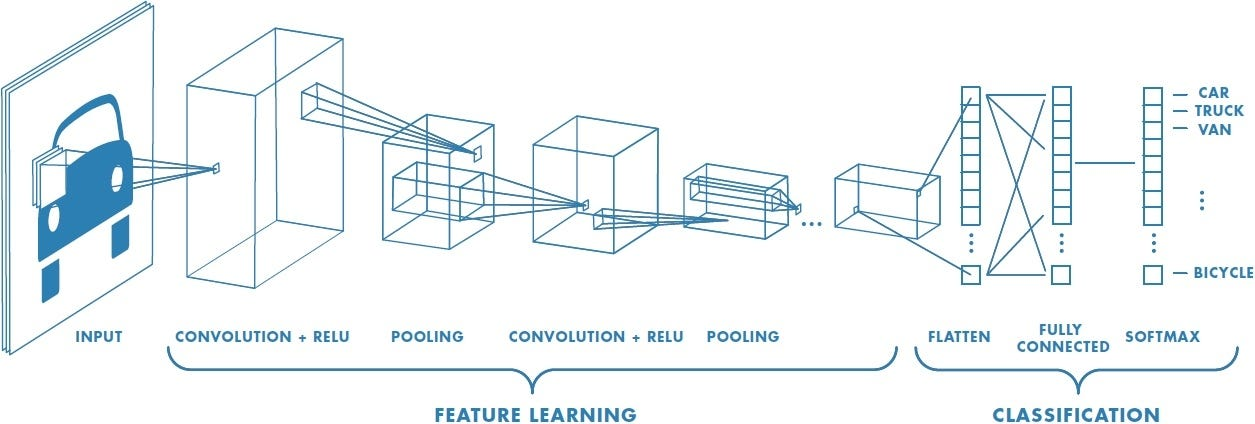
\includegraphics [width=\textwidth]{image/bab2/arsitektur-cnn.jpg}}
    \caption{Arsitektur CNN \citep{wardani2023klasifikasi}}
    \label{Arsitektur CNN}
\end{figure}

\par Pada Gambar \ref{Arsitektur CNN} dapat dilihat bahwa konvolusi merupakan langkah awal dalam pengolahan gambar yang digunakan untuk mengekstraksi fitur penting dari gambar \textit{input}. Dalam konvolusi, hubungan antar piksel dipertahankan dengan cara mengoperasikan kotak kecil pada masukan untuk memahami fitur-fitur gambar. Konvolusi melibatkan operasi matematika linear yang mencakup perkalian antara matriks gambar dan filter (\textit{kernel}) yang merupakan matriks bobot dua dimensi.

\par Fungsi dari lapisan \textit{pooling} adalah untuk secara bertahap mengurangi ukuran representasi spasial gambar, sehingga mengurangi jumlah parameter yang dibutuhkan dalam jaringan. Lapisan \textit{pooling} biasanya ditempatkan di antara lapisan-lapisan konvolusi. Lapisan ini beroperasi secara independen pada setiap peta fitur \citep{monedero2021cyber}.

\par CNN merupakan terobosan besar dalam pengenalan gambar. Mereka belajar langsung dari data gambar, menggunakan pola untuk mengklasifikasikan gambar dan menghilangkan kebutuhan ekstraksi fitur manual. Saat ini, CNN merupakan topik yang menarik dalam \textit{machine learning}, dan telah menunjukkan kinerja yang sangat baik dalam klasifikasi \citep{khan2020survey}. 



\section{\textit{Long Short Term Memory}}

\par \textit{Long Short Term Memory} (LSTM) adalah tipe dari \textit{Recurrent Neural Network} (RNN) yang diciptakan untuk menangani data yang bersifat \textit{sequential} seperti data \textit{time series, speech}, dan \textit{text}. LSTM ini dikembangkan untuk mengatasi masalah \textit{vanishing gradient} yang ada dalam RNN tradisional, yang membuatnya sulit bagi jaringan untuk mempelajari ketergantungan jangka panjang \citep{brownlee2017gentle}.

\par Menurut \citep{alom2019state} LSTM adalah model jaringan saraf yang menggunakan \textit{cell state} untuk menyimpan informasi dari \textit{input} sebelumnya. \textit{Cell state} memiliki tiga gerbang: \textit{input gate} ($i_t$), \textit{forget gate} ($f_t$), dan \textit{output gate} ($o_t$) yang bisa dilihat pada Gambar \ref{diagram_lstm}.

\begin{figure}[H]
\centering
{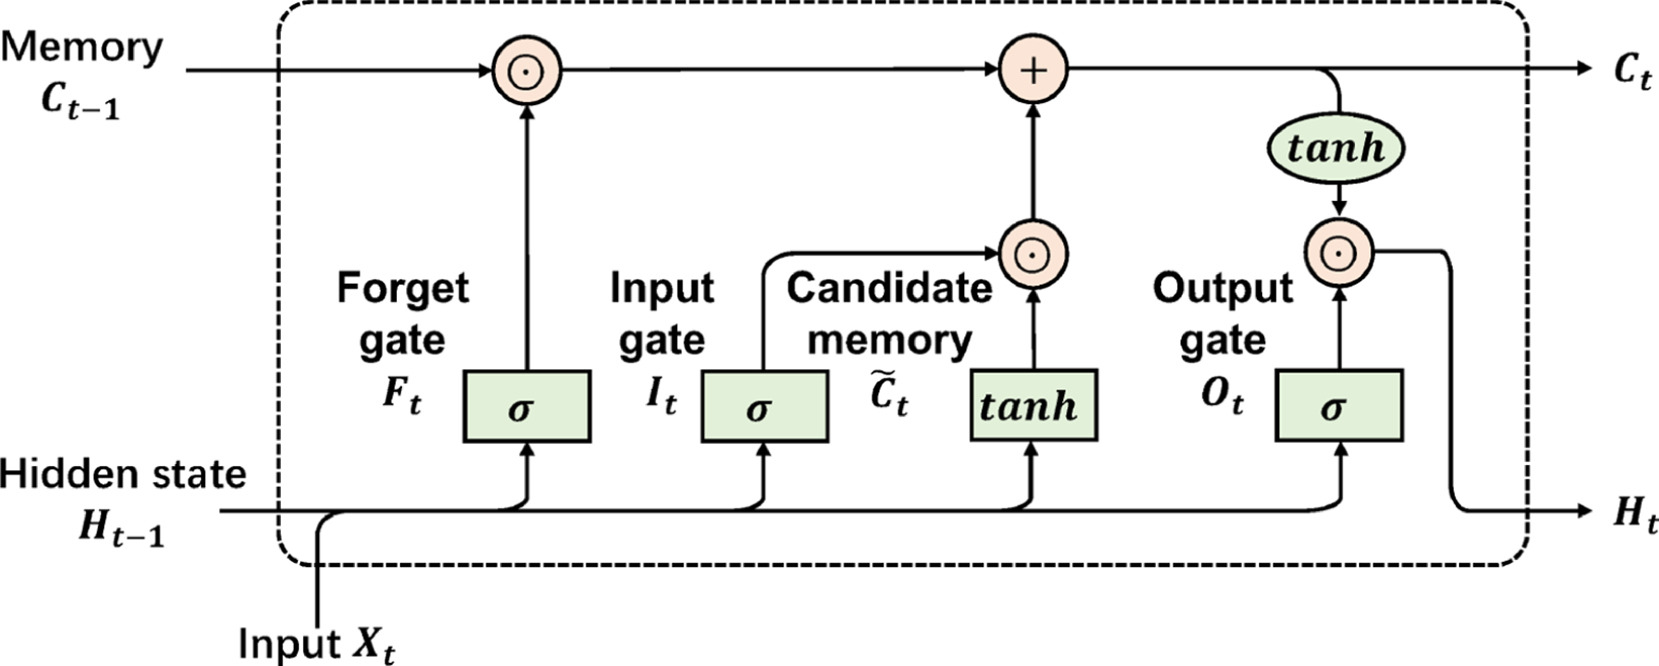
\includegraphics [width=\textwidth]{image/bab2/lstm-architecture.jpg}}
\caption{Arsitektur LSTM \citep{LUO2023107413}}
\label{diagram_lstm}
\end{figure}

\par \textit{Input gate} ($i_t$) digunakan untuk mengontrol pengaruh data yang masuk saat ini terhadap bobot unit tersebut, \textit{forget gate} ($f_t$) bertujuan untuk mengendalikan pengaruh riwayat informasi pada bobot unit saat ini, \textit{output gate} ($o_t$) bertujuan dalam mengendalikan ekspor nilai keadaan unit memori \citep{huang2021fault}.


% \section{\textit{Transformers}}

% \par \textit{Transformers} adalah jenis jaringan saraf yang dapat memproses data berurutan tanpa mengandalkan lapisan \textit{recurrent} dan \textit{convolution}. Pada \textit{transformers} mereka menggunakan mekanisme yang disebut \textit{attention}, yang memungkinkan mereka fokus pada bagian yang paling relevan dari \textit{input} dan \textit{output} pada setiap langkah. \textit{Attention} juga memungkinkan \textit{transformer} untuk menangkap ketergantungan jarak jauh dan informasi kontekstual, yang penting untuk \textit{Natural Language Processing} (NLP). Pada gambar \ref{fig: arsitektur transformer} dapat dilihat bahwa \textit{transformers} terdiri dari \textit{encoder} dan \textit{decoder}. \textit{Encoder} bertugas untuk mengubah teks \textit{input} menjadi urutan representasi tersembunyi, yang disebut \textit{embedding}. \textit{Decoder} bertugas untuk mengambil \textit{embedding} dan menghasilkan teks \textit{output}, satu token pada satu waktu. \textit{Encoder} dan \textit{decoder} terdiri dari beberapa lapisan yang terdiri dari dua sub-lapisan. Sub-lapisan pertama adalah \textit{multi-head self-attention layer}, dan sub-lapisan kedua adalah \textit{feed-forward neural network}. \textit{Multi-head self-attention layer} bertugas untuk mengambil representasi teks \textit{input} dan menghasilkan representasi teks \textit{output} yang lebih baik. \textit{Feed-forward neural network} bertugas untuk mengubah representasi teks \textit{output} menjadi representasi teks \textit{output} yang lebih baik \citep{vaswani2017attention}.

% \begin{figure}[H]
%     \centering
%     {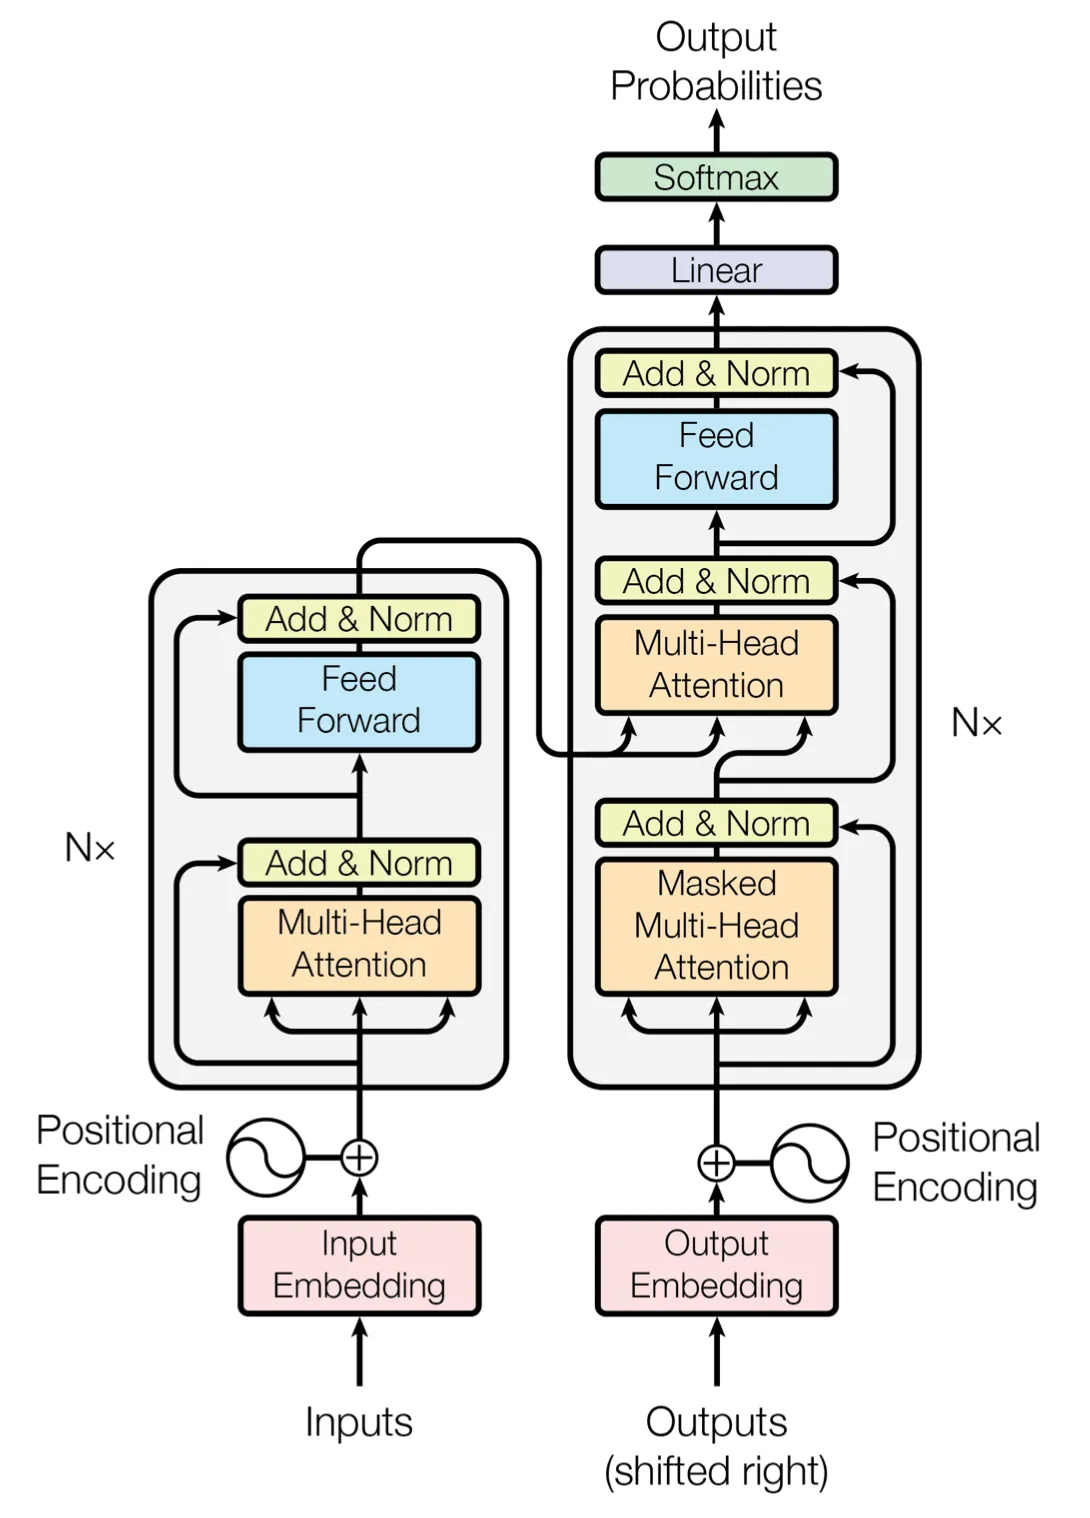
\includegraphics [width = 9cm, height= 15cm]{image/bab2/transformers.png}}
%     \caption{Arsitektur \textit{transformers} \citep{vaswani2017attention}}
%     \label{fig: arsitektur transformer}
% \end{figure}



% \subsection{\textit{Bidirectional Encoder Representation From Transformers} (BERT)}

% \par \textit{Bidirectional Encoder Representation From Transformers} (BERT) adalah 

% \subsection{\textit{Vision Transformer} (ViT)}

% \textit{Vision Transformer} (ViT) adalah model yang diciptakan untuk tugas \textit{computer vision}. Model ini menggunakan arsitektur \textit{transformer} untuk menangani tugas-tugas \textit{computer vision} seperti klasifikasi gambar, deteksi objek, dan segmentasi gambar. ViT mampu mengakses informasi global dan berinteraksi dengan elemen-elemen dalam gambar dengan baik, dan telah menunjukkan hasil yang tinggi dalam berbagai tugas \textit{computer vision}. \par Pada gambar \ref{fig: arsitektur vit} \citep{dosovitskiy2010image}.

% \begin{figure}[H]
%     \centering
%     {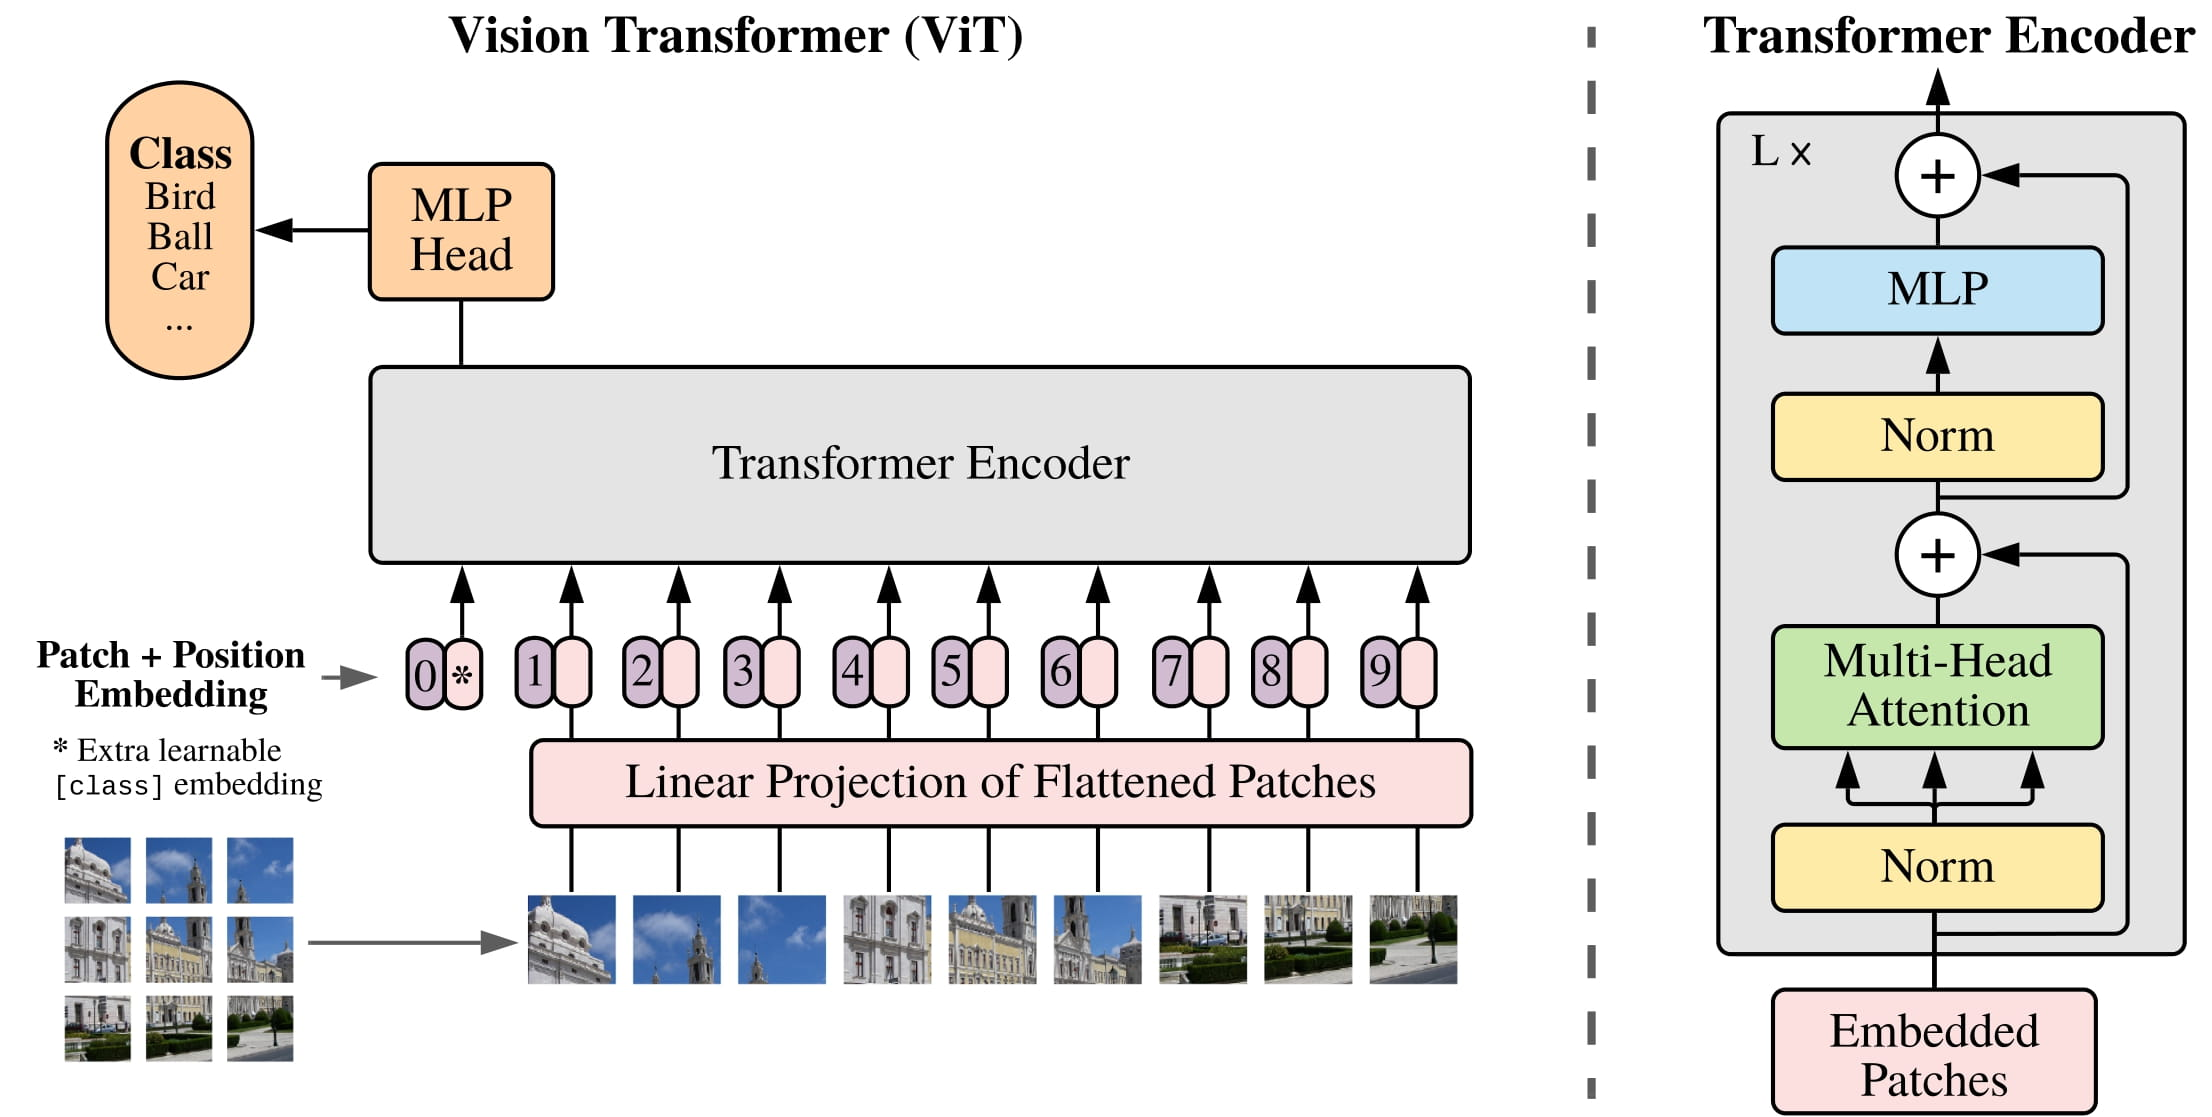
\includegraphics [width=\textwidth]{image/bab2/vit_architecture.jpg}}
%     \caption{Arsitektur ViT \citep{dosovitskiy2010image}}
%     \label{fig: arsitektur vit}
% \end{figure}







\section{\textit{Transfer Learning}}

\par \textit{Transfer learning} digunakan untuk meningkatkan pembelajaran dari satu domain dengan mentransfer informasi dari domain terkait. Kita dapat mengambil pengetahuan dunia nyata non-teknis untuk memahami mengapa \textit{transfer learning} memungkinkan. Pertimbangkan contoh dua orang yang ingin belajar bermain piano. Satu orang tidak memiliki pengalaman sebelumnya dalam bermain musik, dan orang lain memiliki pengetahuan musik yang luas melalui bermain gitar. Orang dengan latar belakang musik yang luas akan dapat belajar piano dengan lebih efisien dengan mentransfer pengetahuan musik yang sudah dipelajari sebelumnya ke tugas belajar bermain piano. Satu orang dapat mengambil informasi dari tugas yang sudah dipelajari sebelumnya dan menggunakannya secara bermanfaat untuk belajar tugas yang terkait \citep{pan2009survey}.


\par \textit{Transfer learning} pada \textit{Artificial Neural Network} (ANN) bisa dibayangkan seperti seseorang yang belajar menjadi lebih mudah, cepat, dan akurat dalam memahami tugas dan konsep baru jika mereka sudah memiliki pengalaman belajar yang serupa dengan konsep baru yang ingin dipelajari. Ini mirip dengan bagaimana seorang individu dapat lebih mudah memahami fisika setelah belajar matematika atau bagaimana seseorang dapat lebih lancar mengendarai truk setelah menguasai kemampuan mengemudi mobil. Pada dasarnya \textit{transfer learning} terjadi ketika pemahaman tentang suatu konteks dipengaruhi oleh pemahaman sebelumnya tentang konteks yang mirip \citep{cirecsan2012transfer}. Intinya adalah bahwa \textit{transfer learning} memungkinkan kita untuk menggunakan pengetahuan yang sudah ada untuk memecahkan masalah baru seperti yang ditunjukkan pada Gambar \ref{transfer_learning}.

\begin{figure}[H]
\centering
{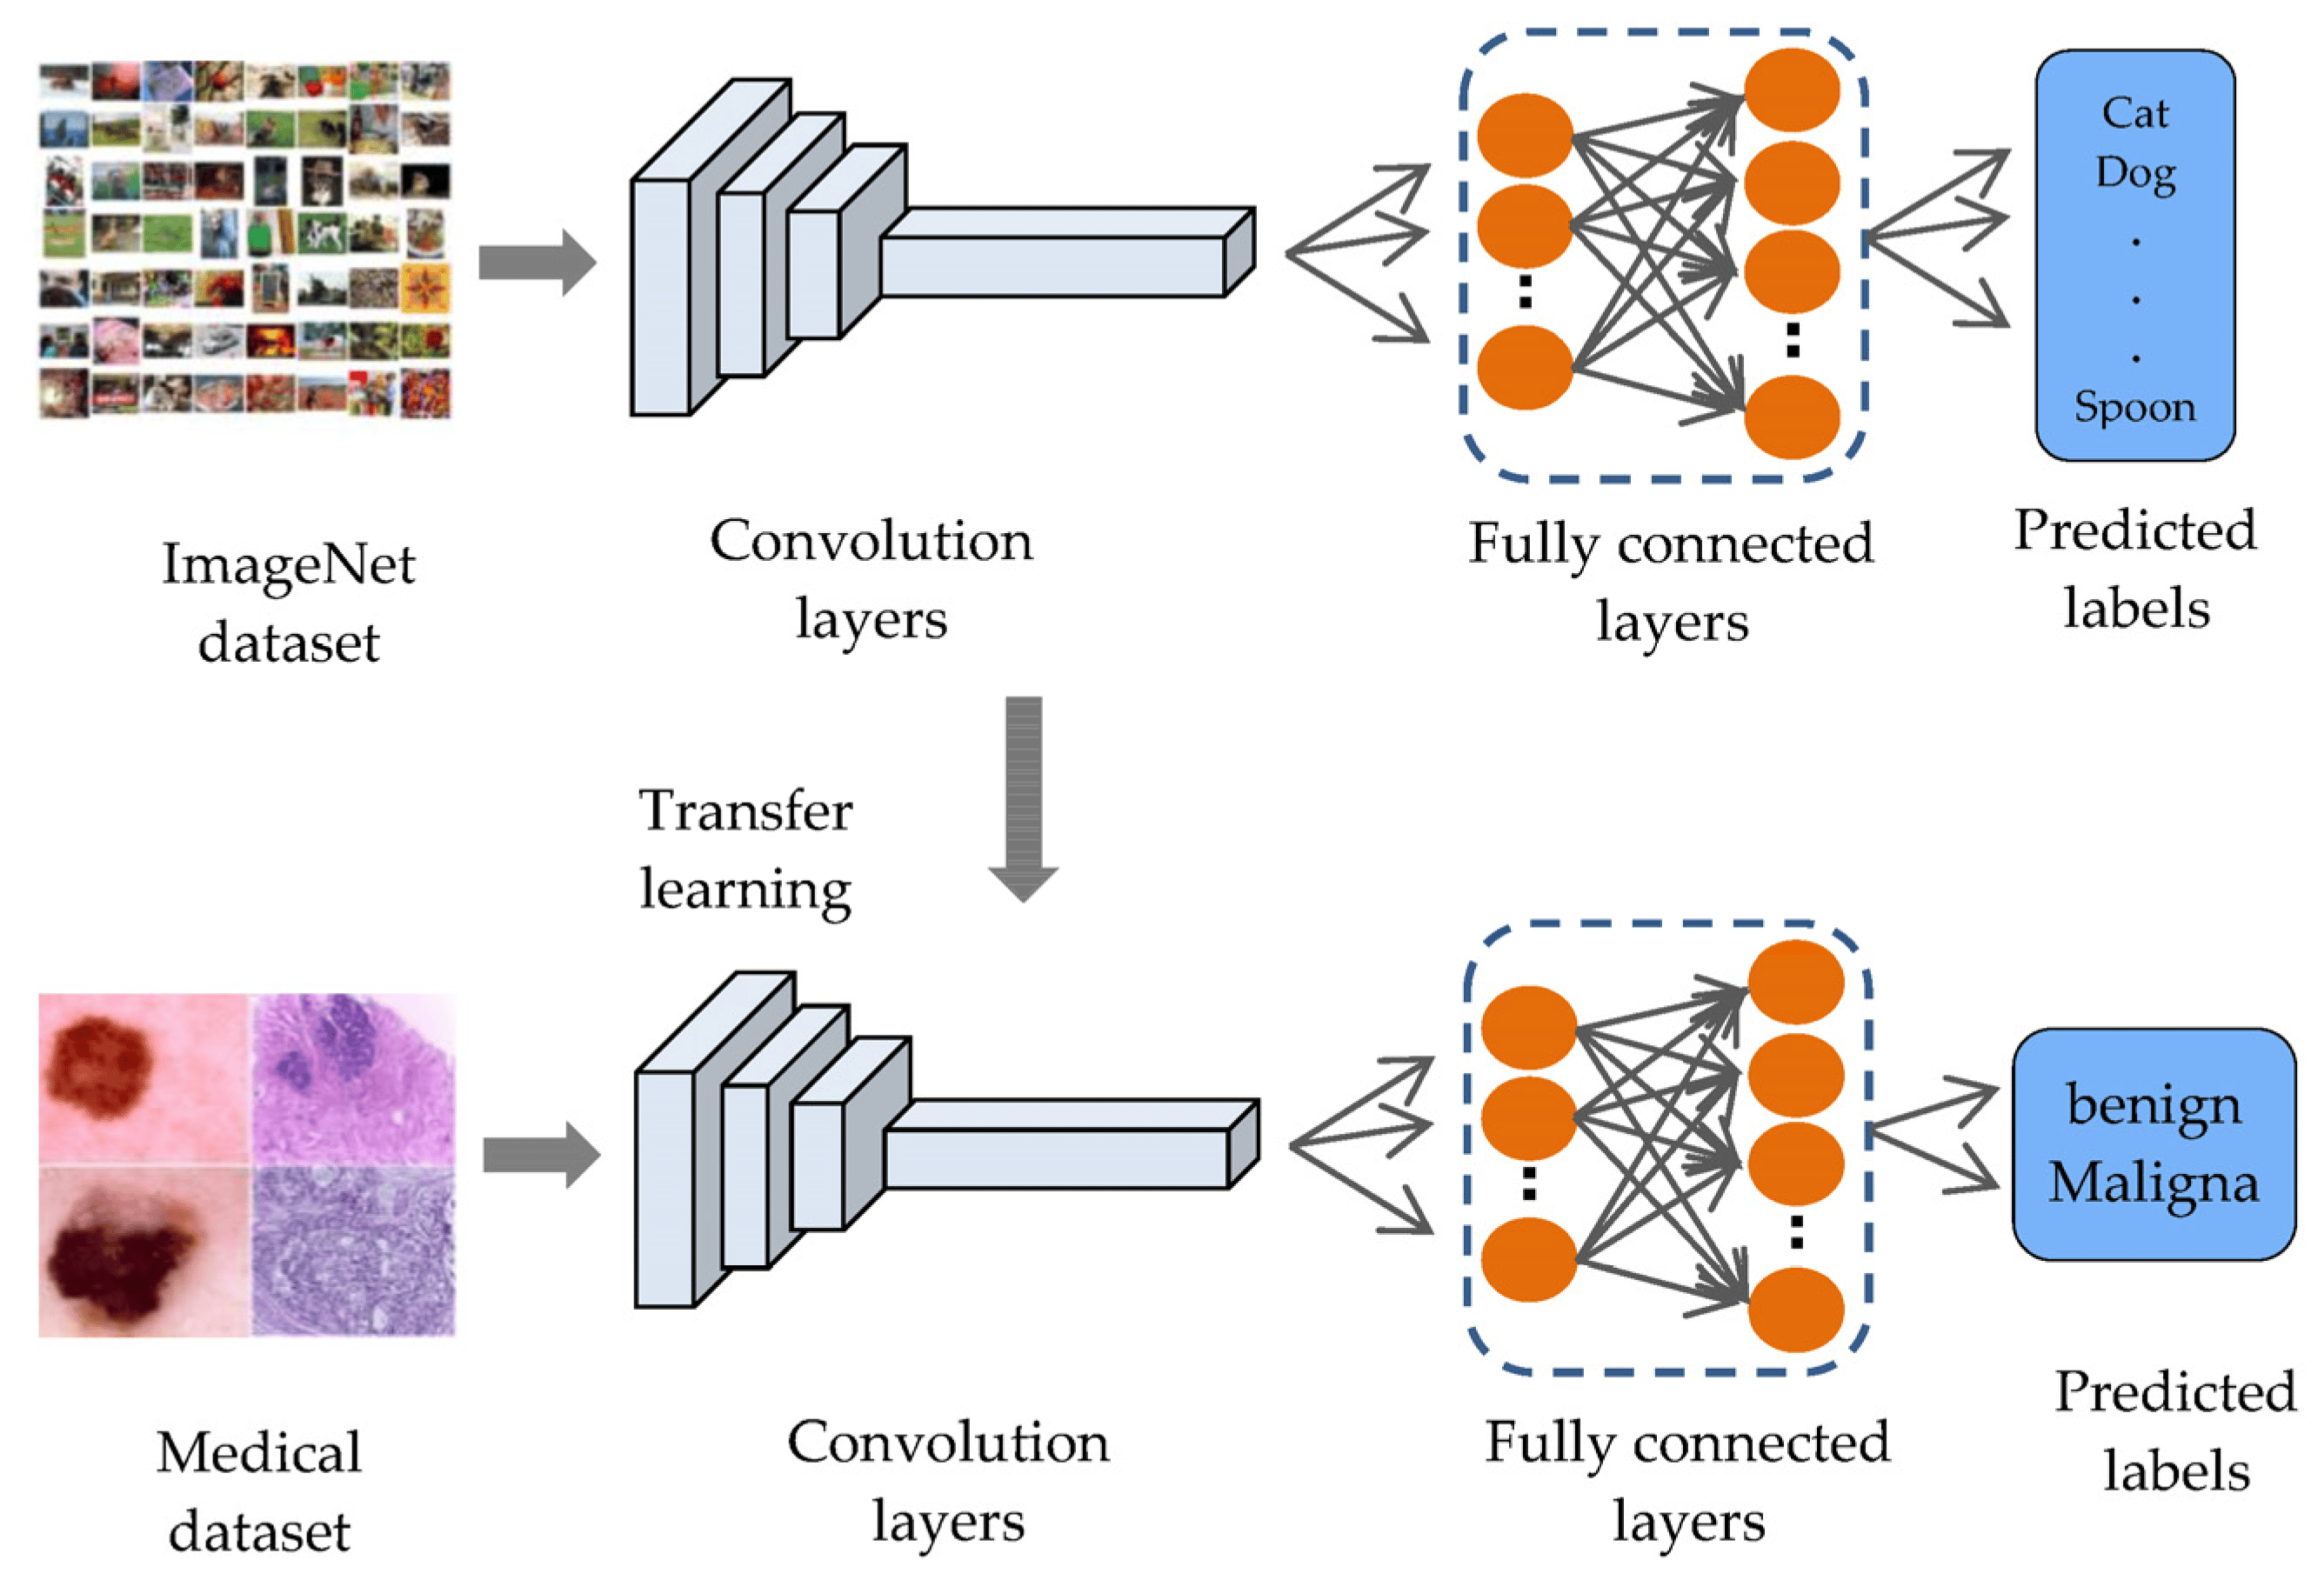
\includegraphics [width = 14cm, height= 8cm]{image/bab2/transfer-learning.png}}
\caption{Konsep penggunaan \textit{transfer learning} \citep{mukhlif2023incorporating}}
\label{transfer_learning}
\end{figure}

\par Model dasar yang digunakan dalam \textit{transfer learning} adalah \textit{pre-trained} model, dimana bobot di seluruh jaringan saraf tiruan sudah disesuaikan untuk data tertentu. Ini memungkinkan model untuk memiliki pemahaman yang lebih mendalam tentang fitur dasar dan fitur tingkat tinggi yang dapat mempercepat proses pelatihan. Secara konsisten, model jaringan saraf yang telah dilatih sebelumnya memberikan hasil prediksi yang lebih tepat dibandingkan dengan jaringan saraf yang dimulai dengan bobot-bobot yang diinisiasi secara acak dalam konteks masalah yang melibatkan data yang sudah memiliki label \citep{cirecsan2012transfer}.


\par VGG19 merupakan salah satu model \textit{pre-trained} yang digunakan dalam penelitian ini. VGG19 adalah model CNN yang memiliki 19 lapisan. Model ini dilatih pada \textit{dataset} ImageNet yang memiliki 1000 kelas dan 1,2 juta gambar. Model ini memiliki 16 lapisan konvolusi dan 3 lapisan \textit{fully connected}. Model ini memiliki 138 juta parameter dan 20 miliar operasi \citep{simonyan2014very}. Arsitektur VGG19 dapat dilihat pada Gambar \ref{Arsitektur VGG19}.


\begin{figure}[H]
    \centering
    {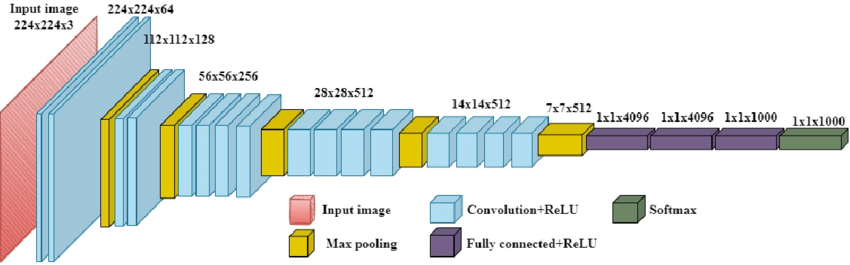
\includegraphics [width=\textwidth]{image/bab2/vgg19.jpeg}}
    \caption{Arsitektur VGG19 \citep{nguyen2022vgg} }
    \label{Arsitektur VGG19}
\end{figure}

\par \textit{Bootstrapping Language-Image Pre-training for Unified Vision-Language Understanding and Generation} (BLIP) adalah sebuah kerangka dari \textit{Vision Language Pre-Training} (VLP). BLIP mampu melakukan berbagai tugas \textit{multimodal} seperti \textit{Visual Question Answering} (VQA), \textit{image captioning}, dan lain-lain. Dalam hal ini, BLIP mengusulkan sebuah model \textit{multimodal mixture of encoder-decoder} yang dapat beroperasi secara fleksibel sebagai \textit{encoder} dan \textit{decoder} untuk berbagai tugas penglihatan bahasa. BLIP mampu memajukan \textit{pre-training} terunifikasi untuk transfer pembelajaran lintas tugas \textit{vision-language}. Berikut ini dapat dilihat arsitektur pada BLIP pada Gambar \ref{Arsitektur BLIP}.

\begin{figure}[H]
    \centering
    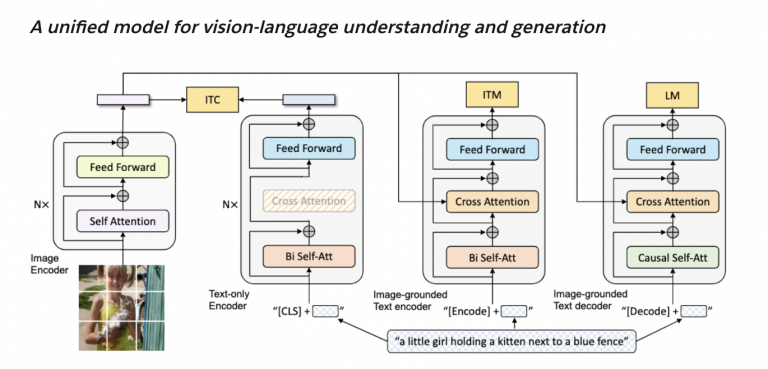
\includegraphics[width=\textwidth]{image/bab2/arsitektur-blip.png}
    \caption{Arsitektur BLIP \citep{li2022blip}}
    \label{Arsitektur BLIP}
\end{figure}

\par BLIP memiliki tiga fungsionalitas yang dapat dilihat sebagai berikut:

\begin{enumerate}

    \item{\textit{Unimodal encoder} yang memisahkan proses \textit{encode} gambar dan teks. \textit{Image encoder} didasarkan pada \textit{Vision Transformer} (ViT), sementara \textit{encoder} teks mirip dengan \textit{Bidirectional Encoder Representation from Transformer} (BERT). Disini, terdapat token khusus [CLS] yang ditambahkan di awal \textit{input} teks untuk merangkum kalimat.}

    \item{\textit{Image-grounded text encoder} yang bertujuan memasukkan informasi visual ke dalam \textit{encoder} teks. Pada bagian ini dilakukan dengan menyisipkan lapisan \textit{cross-attention} antara lapisan \textit{self-attention} dan jaringan \textit{feed-forward} untuk setiap blok transformer dari \textit{encoder} teks. Pada bagian ini terdapat token khusus yaitu [Encode] yang ditambahkan ke teks, dan \textit{embedding output} dari [Encode] ini digunakan sebagai representasi multimodal dari pasangan gambar dan teks.}

    \item{\textit{Image grounded text decoder} memodifikasi \textit{encoder} teks dengan menggantikan lapisan \textit{bidirectional self-attention} dengan lapisan \textit{causal self-attention}. Di bagian ini, token khusus [Decode] digunakan untuk menandai awal dari sebuah urutan.}

\end{enumerate}

\par Pada gambar \ref{Arsitektur BLIP} dijelaskan tiga tujuan dari arsitektur BLIP. Penjelasan tiga tujuan BLIP dapat dilihat sebagai berikut:

\begin{enumerate}
    \item{\textit{Image-Text Contrastive Loss} (ITC) bertujuan mengaktifkan \textit{unimodal encoder}. ITC mendorong keselarasan dalam ruang fitur transformer visual dan transformer teks dengan memastikan pasangan gambar dan teks yang positif memiliki representasi yang mirip dibandingkan dengan pasangan negatif.}

    \item{\textit{Image-Text Matching Loss} (ITM) bertujuan dalam mengaktifkan \textit{encoder} teks berdasarkan gambar. Bagian ini merupakan tugas klasifikasi biner dimana model memprediksi apakah pasangan gambar dan teks cocok atau tidak cocok berdasarkan fitur \textit{multimodal} mereka.}

    \item{\textit{Language Modelling Loss} (LM) bertujuan mengaktifkan \textit{decoder} teks berdasarkan gambar. Ini berfokus menghasilkan deskripsi teks yang dikondisikan pada gambar yang diberikan.}


\end{enumerate}

\par Intinya, BLIP menggunakan model serbaguna yang dapat menyatukan informasi visual ke dalam pemrosesan teks. Selama tahap pra-pelatihan, BLIP secara simultan mengoptimalkan tujuan keselarasan representasi visual dan teks, pencocokan pasangan gambar dan teks, serta pembangkitan deskripsi dalam bahasa dan gambar \citep{li2022blip}.

% \par ViLT (\textit{Vision-and-Language Transformer}) adalah suatu struktur model yang menggabungkan informasi dari unsur visual dan teks untuk berbagai tugas yang melibatkan unsur visual dan bahasa, seperti penggantian keterangan gambar (\textit{image captioning}), menjawab pertanyaan visual (\textit{visual question answering}), dan lain-lain. ViLT merupakan perkembangan lebih lanjut dari model VLP (\textit{Vision and Language Pre-training}) dan diciptakan dengan tujuan untuk mengatasi beberapa masalah yang ada pada model VPL sebelumnya. Keunggulan dari model ViLT terletak pada kemampuannya yang lebih baik dibandingkan dengan model VLP, yang disebabkan oleh pendekatan yang lebih sederhana dan efisien dalam memproses informasi visual masukan, berbeda dengan model VPL yang memerlukan ekstraksi fitur gambar yang kompleks, seperti deteksi objek dan arsitektur konvolusi. Arsitektur ViLT mengurangi ketergantungan pada ekstraksi fitur gambar yang rumit dan mengusulkan suatu pendekatan yang lebih langsung dalam memproses informasi visual masukan, sehingga menghasilkan kecepatan yang lebih tinggi, tetapi tetap mempertahankan atau meningkatkan kinerja dalam tugas-tugas turunan yang melibatkan unsur visual dan bahasa \citep{kim2021vilt}. Struktur arsitektur ViLT dapat dilihat pada gambar \ref{Arsitektur ViLT}.

% \begin{figure}[H]
%     \centering
%     {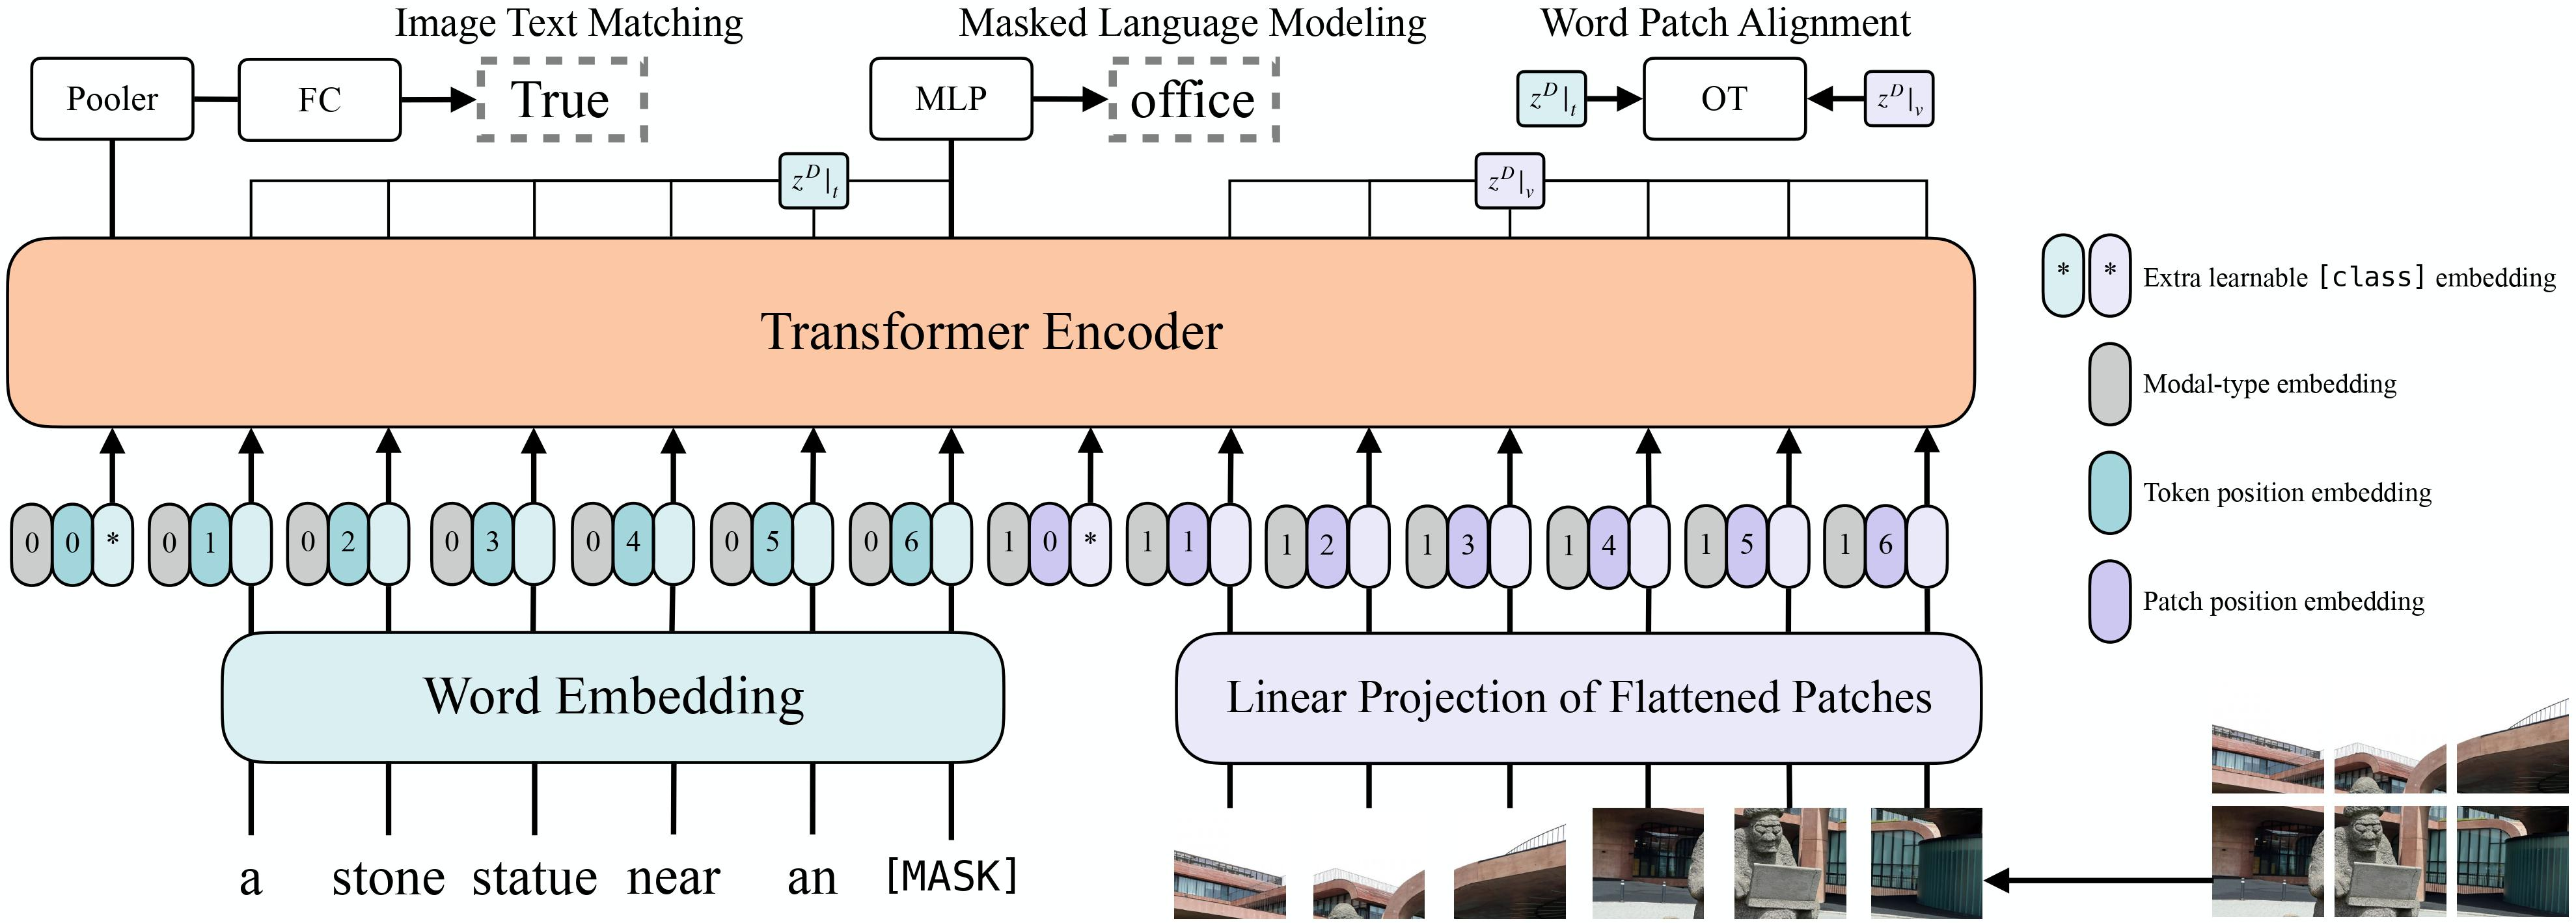
\includegraphics [width = 15cm, height= 6cm]{image/bab2/vilt_architecture.jpg}}
%     \caption{Arsitektur ViLT \citep{kim2021vilt} }
%     \label{Arsitektur ViLT}
% \end{figure}


\section{Matriks Evaluasi}

\par Matriks evaluasi yang digunakan dalam menilai kinerja model \textit{medical} VQA dapat dikategorikan menjadi dua jenis, yaitu \textit{classification-based metrics} dan \textit{language-based metrics}. Pada umumnya metrik yang digunakan pada kasus klasifikasi, seperti akurasi dan \textit{F1-score}. Metrik ini memperlakukan jawaban sebagai hasil dari klasifikasi dan menghitung pencocokan yang tepat untuk akurasi, presisi, \textit{recall} dan lain-lain. Sedangkan metrik yang digunakan pada kasus \textit{language-based} bertujuan untuk mengevaluasi tugas seperti penerjemah, \textit{image captioning}, VQA, dan lain-lain. \textit{Dataset} seperti VQA-Med-2018, VQA-Med-2019, PathVQA, VQA-Med-2020, dan VQA-Med-2021 menggunakan metrik \textit{language-based} seperti \textit{BLEU}, untuk mengevaluasi kinerjanya \citep{lin2023medical}.

\par \textit{Confusion matrix} adalah suatu alat pengukuran kinerja yang digunakan dalam konteks masalah klasifikasi pada pembelajaran mesin. Matriks ini terdiri dari tabel memberikan gambaran visual dan ringkasan mengenai kinerja algoritma klasifikasi. Tiap baris dalam matriks mencerminkan contoh dalam kelas aktual, sementara setiap kolom mencerminkan contoh dalam kelas yang diprediksi. \textit{Confusion matrix} sangat bermanfaat untuk menilai efektivitas suatu model, terutama ketika terdapat ketidakseimbangan jumlah observasi antar kelas atau ketika menghadapi lebih dari dua kelas dalam suatu \textit{dataset}. \textit{Confusion matrix} merefleksikan nilai \textit{True Positive} (TP) yang menunjukkan klasifikasi yang tepat pada kelas yang relevan, nilai \textit{False Positive} (FP) yang mencerminkan klasifikasi di kelas yang seharusnya tidak relevan, nilai \textit{False Negative} (FN) yang menunjukkan klasifikasi di kelas yang salah ketika seharusnya relevan, dan nilai \textit{True Negative} (TN) yang mencerminkan klasifikasi yang benar di kelas yang tidak relevan. Gambar \textit{confusion matrix} dapat dilihat pada Gambar \ref{Confusion Matrix} \citep{KULKARNI202083}.

\begin{figure}[H]
    \centering
    {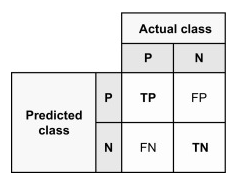
\includegraphics [width = 8cm, height= 5cm]{image/bab2/conf-matrix.png}}
    \caption{\textit{Confusion matrix} \citep{KULKARNI202083}}
    \label{Confusion Matrix}
\end{figure}

\subsection{Akurasi}

\par Pada umumnya akurasi adalah metrik yang mengukur perbandingan antara jumlah prediksi yang benar dengan jumlah total kasus yang dievaluasi \citep{hossin2015review}. Pada persamaan \ref{rumus-accuracy} menunjukkan bahwa rumus dari akurasi adalah jumlah prediksi yang benar dibagi dengan total prediksi yang dilakukan.

% Rumus Accuracy
\begin{equation}
    % rumus accuracy
    Akurasi = \frac{TP + TN}{TP + TN + FP + FN}
    \label{rumus-accuracy}
\end{equation}

% keterangan rumus accuracy
\begin{itemize}
    \item TP (\textit{True Positive}) adalah jumlah prediksi yang benar positif.
    \item TN (\textit{True Negative}) adalah jumlah prediksi yang benar negatif.
    \item FP (\textit{False Positive}) adalah jumlah prediksi yang salah positif.
    \item FN (\textit{False Negative}) adalah jumlah prediksi yang salah negatif.

\end{itemize}

\subsection{\textit{Bilingual Evaluation Understudy}}

\par \textit{Bilingual Evaluation Understudy} (BLEU) adalah metrik yang digunakan untuk mengukur kesamaan pada frase (n-grams) antara dua kalimat. BLEU adalah metrik original untuk penerjemah mesin dan juga bisa digunakan untuk tugas seperti pembuatan laporan medis \citep{li2021ffa}.

\par BLEU adalah metrik yang digunakan untuk mengevaluasi kualitas sistem terjemahan mesin \citep{papineni2002bleu}. Ini mengukur kemiripan antara terjemahan yang dihasilkan oleh mesin dan satu atau lebih referensi terjemahan menggunakan metrik presisi yang dimodifikasi dan hukuman singkat yang dimodifikasi dan \textit{brevity penalty} yang dimodifikasi.

\begin{equation}
    \text{BLEU} = \text{BP} \times \exp\left(\sum_{n=1}^{N} w_n \log p_n\right) 
    \label{rumus-bleu}
\end{equation}


% keterangan rumus BLEU

\begin{itemize}
    \item $BP$ adalah \textit{brevity penalty}.
    \item $N$ adalah jumlah maksimal n-gram.
    \item $w_n$ adalah bobot untuk n-gram.
    \item $p_n$ adalah presisi n-gram.

\end{itemize}

\par Berdasarkan persamaan \ref{rumus-bleu} \textit{Brevity Penalty} (BP)  menghukum jawaban singkat, $w_n$ adalah bobot antara 0 dan 1 untuk $\log p_n$ dan $\sum_{n=1}^{N} w_n = 1$, $p_n$ adalah nilai rata-rata geometris dari presisi n-gram yang dimodifikasi, dan N adalah panjang maksimum n-gram.

\par BLEU memiliki beberapa variasi, seperti BLEU-1, BLEU-2, BLEU-3, dan seterusnya. Variasi ini menunjukkan jumlah n-gram yang digunakan dalam perhitungan BLEU. Semakin tinggi nilai BLEU, semakin baik kualitas terjemahan mesin tersebut. Nilai BLEU berkisar dari 0 hingga 100, di mana 100 menunjukkan terjemahan yang sempurna. Berikut adalah penjelasan mengenai berbagai variasi BLEU:

\begin{enumerate}

    \item BLEU-1 adalah variasi dasar dari metrik BLEU yang hanya mempertimbangkan \textit{unigram} (kata tunggal). Perhitungan BLEU-1 mengukur seberapa baik kata-kata dalam hasil terjemahan sesuai dengan kata-kata dalam kalimat referensi tanpa mempertimbangkan urutan kata.

    \item BLEU-2 memperluas perhitungan dengan menggunakan \textit{bigram} (pasangan kata). Dalam BLEU-2, selain mempertimbangkan kesesuaian \textit{unigram}, juga diperiksa kesesuaian pasangan kata dalam hasil terjemahan dan kalimat referensi. Hal ini memberikan evaluasi yang lebih baik terhadap struktur kalimat terjemahan.

    \item BLEU-3 melangkah lebih jauh dengan menggunakan \textit{trigram} (tiga kata berturut-turut). Disini, evaluasi BLEU-3 memperhitungkan kesesuaian \textit{trigram} antara hasil terjemahan dan kalimat referensi. Semakin panjang n-gram yang digunakan, semakin ketat evaluasi terhadap kualitas terjemahan, karena memperhatikan konteks yang lebih luas dalam kalimat.

\end{enumerate}

\par Kesimpulannya, variasi-variasi ini menunjukkan bahwa dengan meningkatnya nilai "n" dalam n-gram, evaluasi terhadap terjemahan mesin menjadi lebih komprehensif dan memperhitungkan konteks yang lebih luas dalam kalimat \citep{papineni2002bleu}.






\par Deskripsi BLEU berbeda tergantung pada rentang nilai yang ada. Detail deskripsi untuk masing-masing rentang nilai BLEU dapat ditemukan di Tabel \ref{tabel-bleu} \citep{lavie2010evaluating}.

\begin{table}[H]
    \centering
    \caption{Deskripsi dari masing-masing nilai BLEU}
    \label{tabel-bleu}
    \begin{tabular}{|l|l|}
    \hline
    \textbf{Nilai BLEU} & \textbf{Deskripsi}                                                    \\ \hline
    \textless\ 10       & Hampir tidak dapat dipahami                                           \\ \hline
    10 - 19             & Sulit untuk mendapatkan intisari kalimat                              \\ \hline
    20 - 29             & Inti kalimat jelas, tetapi memiliki banyak kesalahan pada tata bahasa \\ \hline
    30 - 39             & Dapat dimengerti sebagai penerjemah kalimat yang baik                 \\ \hline
    40 - 49             & Terjemahan kalimat berkualitas tinggi                                 \\ \hline
    50 - 59             & Terjemahan kalimat sangat berkualitas dan memadai                     \\ \hline
    \textgreater\ 60    & Kemampuan menerjemah sering lebih bagus dari manusia                  \\ \hline
    \end{tabular}
\end{table}


\section{\textit{Visual Question Answering}}

\par \textit{Visual Question Answering} (VQA) adalah suatu tugas tentang bagaimana menjawab pertanyaan bebas pada sebuah gambar. Karena membutuhkan pemahaman bahasa yang mendalam tentang pertanyaan dan kemampuan untuk mengaitkannya dengan berbagai objek yang ada dalam gambar. Ini adalah tugas yang ambisius dan memerlukan teknik dari baik \textit{computer vision} dan \textit{natural language processing} \citep{hildebrandt2020scene}.

\par Salah satu contoh percobaan yang dilakukan oleh \citep{antol2015vqa}, mereka menerapkan \textit{baseline} \textit{Vanilla} VQA model yang dimana sebagai tolak ukur untuk metode \textit{deep learning}. Model ini menggunakan CNN untuk ekstraksi fitur dan jaringan LSTM atau \textit{recurrent network} untuk pemrosesan bahasa. Fitur-fitur ini digabungkan menggunakan suatu operasi untuk membentuk satu fitur bersama, yang digunakan untuk mengklasifikasikan salah satu jawaban seperti yang ditunjukkan dalam Gambar \ref{exp: visual question answering}.

\begin{figure}[H]
    \centering
    {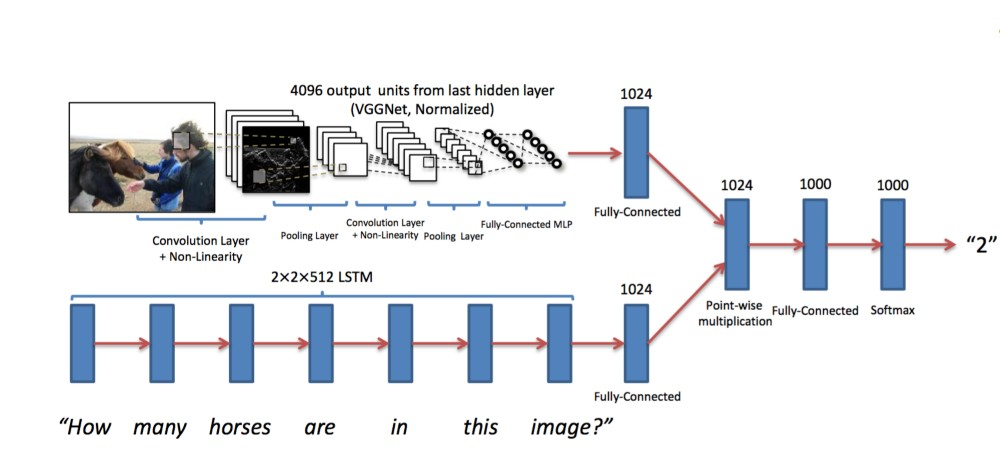
\includegraphics [width=\textwidth]{image/bab2/vqa.jpeg}}
    \caption{Vanilla VQA \textit{network} model \citep{srivastava2021visual}}
    \label{exp: visual question answering}
\end{figure}

% \par Lalu ada \textit{baseline} model dikenali oleh \citep{teney2018tips}. Model ini menggunakan deteksi objek pada VQA model dan memenangkan tantangan untuk tugas VQA pada tahun 2017. Model ini membantu mempersempit fitur-fitur dan memberikan perhatian yang lebih baik pada gambar. Model ini menggunakan arsitektur R-CNN dan menunjukkan peningkatan yang signifikan dalam akurasi dibandingkan dengan arsitektur lainya. Berikut adalah gambar \ref{exp: teney model} yang menunjukkan arsitektur pada model.

% \begin{figure}[H]
%     \centering
%     {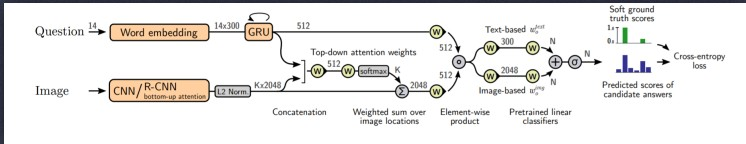
\includegraphics [width = 12cm, height= 3cm]{image/bab2/teney_model.jpeg}}
%     \caption{Teney Model \citep{srivastava2021visual}}
%     \label{exp: teney model}
% \end{figure}

\par VQA telah menarik minat besar dan mengalami perkembangan oleh para peneliti dan ilmuwan dari seluruh dunia. Tren terbaru yang diamati adalah dalam pengembangan \textit{dataset} yang terlihat semakin mirip dengan dunia nyata dengan menggabungkan pertanyaan dan jawaban seputar kehidupan nyata. Tren terkini juga terlihat dalam pengembangan model \textit{deep learning} yang lebih canggih dengan lebih baik memanfaatkan petunjuk visual dan petunjuk teks melalui berbagai cara. Kinerja model terbaik saat ini masih tertinggal dan hanya sekitar 60-70\% saja. Oleh karena itu, masih merupakan masalah yang terbuka untuk mengembangkan model \textit{deep learning} yang baik serta \textit{dataset} yang lebih menantang untuk \textit{visual question answering} \citep{srivastava2021visual}. 

\par Dalam mengembangkan sistem VQA diperlukan dua cabang ilmu seperti yang sudah dijelaskan yaitu \textit{computer vision} dan \textit{natural language processing} dikarenakan melibatkan gambar dan pertanyaan teks yang terkait \citep{teney2017visual}.

\subsection{\textit{Computer Vision}}

\par \textit{Computer Vision} (CV) bisa diartikan sebagai sekelompok teknik yang digunakan untuk mengumpulkan, memproses, menganalisis, dan memahami data yang kompleks dan berdimensi tinggi dari lingkungan sekitar kita. Tujuannya adalah untuk menjalani eksplorasi ilmiah dan teknis yang melibatkan pemahaman dan interpretasi data visual. Secara sederhana, CV memungkinkan komputer atau sistem komputasi untuk melihat, menginterpretasi, dan merespons informasi visual dari dunia nyata. Teknologi ini memiliki berbagai aplikasi, termasuk pengenalan objek, deteksi pola, dan pengolahan citra, serta mendukung berbagai bidang seperti kecerdasan buatan, penglihatan mesin, dan analisis data visual \citep{jahne1999handbook}.


\subsection{\textit{Natural Language Processing}}

\par \textit{Natural Language Processing} (NLP) adalah cabang ilmu dari pembelajaran mesin yang berfokus pada teks. Metode ini memungkinkan suatu komputer untuk menganalisis, memahami, dan menghasilkan makna dari bahasa manusia dengan cerdas dan bermanfaat. Dengan memanfaatkan NLP, pengembang dapat mengorganisir dan menyusun pengetahuan untuk menjalankan tugas-tugas seperti rangkuman otomatis, terjemahan, pengenalan entitas bernama, ekstraksi hubungan, analisis sentimen, pengenalan ucapan, dan segmentasi topik \citep{agarwal2019overview}.

\par Dalam NLP \textit{word embedding} merupakan representasi dari suatu kata. \textit{Embedding} digunakan dalam analisis teks. Biasanya, representasi tersebut berupa vektor nilai rill yang mengkodekan makna kata sedemikian rupa sehingga kata-kata yang lebih dekat dalam ruang vektor diharapkan memiliki makna yang mirip \citep{teller2000speech}. \textit{Global Vectors for Word Representation} (GloVe) adalah metode untuk membuat representasi kata. GloVe adalah algoritma \textit{unsupervised learning} yang memperoleh representasi vektor untuk kata-kata dengan melatih pada statistik kumulatif keterjadian bersama global kata-kata dari suatu korpus. Representasi yang dihasilkan menunjukkan struktur sublinear menarik dari ruang vektor kata, memungkinkan kata-kata dengan makna serupa berada lebih dekat dalam ruang vektor. Dalam hal ini, GloVe digunakan untuk membangun fitur \textit{embedding} kata semantik dan telah digunakan dalam berbagai tugas dalam bidang NLP \citep{pennington2014glove}.

\section{\textit{Medical Visual Question Answering Dataset}}

\par \textit{Medical visual question answering dataset} adalah \textit{dataset} yang digunakan untuk melakukan penelitian terkait tugas yang berkaitan dengan \textit{medical visual question answering} \citep{lin2023medical}. \textit{Dataset} ini berisi gambar medis dan pertanyaan yang terkait dengan gambar tersebut. Pada penelitian ini akan digunakan \textit{dataset} PathVQA dan VQA-RAD. Berikut adalah penjelasan dari kedua \textit{dataset} tersebut.

\subsection{PathVQA \textit{Dataset}}

\par \textit{Dataset} PathVQA berisi 32.799 pertanyaan dan jawaban dari 1.670 gambar patologi yang dikumpulkan dari dua buku patologi, yaitu '\textit{Textbook of Pathology}' dan '\textit{Basic Pathology}'. Selain itu, terdapat 3.328 gambar lainnya yang dikumpulkan dari perpustakaan digital PEIR. Dengan demikian, total gambar pada \textit{dataset} ini mencapai 4.998. Rata-rata setiap satu gambar memiliki 6,6 pertanyaan. Jumlah pertanyaan maksimal dan minimal adalah 14 dan 1 berturut-turut. Rata-rata jumlah kata per pertanyaan dan perjawaban adalah 9,5 dan 2,5 berturut-turut. Pada \textit{dataset} ini terdapat 7 kategori pertanyaan, yaitu: \textit{what}, \textit{where}, \textit{when}, \textit{whose}, \textit{how}, \textit{how much/how many}, dan \textit{yes/no}. Pertanyaan dari enam kategori pertama bersifat \textit{open-ended}, sedangkan pertanyaan dari kategori terakhir bersifat \textit{close-ended} '\textit{yes/no}'. Jumlah jawaban '\textit{yes}' dan '\textit{no}' adalah 8.145 dan 8.189 berturut-turut. Pertanyaan pada \textit{dataset} ini mencakup banyak aspek konten visual, termasuk warna, lokasi, penampilan, bentuk, dan lain-lain. Keragaman klinis ini menimbulkan tantangan yang besar bagi model AI dalam menjawab permasalahan pada gambar patologi \citep{xuehai2020pathvqa}.


\subsection{VQA-RAD \textit{Dataset}}

\par \textit{Dataset} VQA-RAD adalah \textit{dataset} yang dibuat secara manual untuk penelitian terkait \textit{Medical Visual Question Answering} (VQA). \textit{Dataset} ini berisi 3.515 pasangan pertanyaan dan jawaban yang dihasilkan oleh para klinisi, serta 315 gambar radiologi yang terbagi merata antara kepala, dada, dan perut. Dengan rata-rata, setiap gambar memiliki 10 pertanyaan terkait. Setiap gambar ini terkait dengan beberapa pertanyaan, yang dikelompokkan ke dalam 11 kategori: kelainan, atribut, modalitas, sistem organ, warna, penghitungan, keberadaan objek/kondisi, ukuran, bidang, penalaran posisional, dan lain-lain. Setengah dari pertanyaan pada \textit{dataset} ini bersifat \textit{close-ended} (\textit{yes/no}), sedangkan setengahnya lagi bersifat \textit{open-ended}. \textit{Dataset} ini merupakan kontribusi berharga dalam pengembangan model VQA di bidang radiologi, dengan pertanyaan-pertanyaan yang disusun oleh para ahli klinis, mencakup berbagai aspek interpretasi gambar medis \citep{lau2018dataset}.



\section{Penelitian Terkait}

\par Penelitian yang dilakukan oleh \citep{xuehai2020pathvqa} berhasil mengatasi tantangan khusus dalam analisis citra patologi dengan menggabungkan metode pemrosesan gambar dan pemrosesan bahasa alami. Mereka melakukan eksperimen dengan tiga metode berbeda. Tiga metode yang digunakan melibatkan integrasi \textit{Gated Recurrent Unit} (GRU) dan Faster R-CNN dengan melibatkan \textit{Bilinear Attention Network}, \textit{Convolutional Neural Network} (CNN) dan \textit{Long Short Term Memory} (LSTM) dengan \textit{compact bilinear pooling}, serta \textit{Stacked Attention Network} (SAN) yang menggabungkan CNN dan LSTM. Pengkodean gambar menggunakan Faster R-CNN dan ResNet-152. Berdasarkan ketiga eksperimen ini menunjukkan bahwa metode pertama mencapai akurasi tertinggi untuk pertanyaan \textit{close-ended} adalah 68,2\% dan mendapatkan nilai BLEU-1, BLEU-2, BLEU-3 sebesar 32,4, 22,8, 17,4 berturut-turut untuk pertanyaan \textit{open-ended}. Metode kedua mencapai akurasi sebesar 57,6\% untuk pertanyaan \textit{close-ended} dan mendapatkan BLEU-1, BLEU-2, BLEU-3, sebesar 13,3, 9,5, 6,8 berturut-turut untuk pertanyaan \textit{open-ended}. Metode ketiga mendapatkan akurasi sebesar 59,4\% untuk pertanyaan \textit{close-ended} dan mendapatkan BLEU-1, BLEU-2, BLEU-3 sebesar 19,2, 17,9, 15,8 berturut-turut untuk pertanyaan \textit{open-ended}. Lalu, hasil yang didapat ketika melakukan pengkodean gambar dengan Faster R-CNN mendapatkan akurasi 62,0\% untuk pertanyaan \textit{close-ended} dan mendapatkan BLEU-1, BLEU-2, BLEU-3 sebesar 24,7, 19,1, 16,5 berturut-turut untuk pertanyaan \textit{open-ended}. Sedangkan ketika menggunakan ResNet-152, mereka mendapatkan akurasi 60,1\% untuk pertanyaan \textit{close-ended} dan BLEU-1, BLEU-2, BLEU-3 sebesar 19,9, 18,0, 16,0 berturut-turut untuk pertanyaan \textit{open-ended} \citep{xuehai2020pathvqa}.

\par Penelitian lain juga dilakukan untuk meningkatkan diagnosis dengan menjawab pertanyaan klinis yang disajikan dengan gambar medis menggunakan model \textit{Contrastive Language Image Pre Training} (CLIP) yang mengintegrasikan pembelajaran \textit{multimodal embedding} melalui pelatihan bersama \textit{image encoder} dan \textit{text encoder} untuk memaksimalkan kemiripan pasangan gambar-teks yang sesuai. Metodenya melibatkan penggunaan \textit{Vision Transformer} (ViT) untuk \textit{image encoder}, pertanyaan dimasukkan ke dalam transformer \textit{encoder} teks, dan penggabungan representasi visual dan teks dalam \textit{decoder multimodal} untuk menghasilkan jawaban otomatis. Uji coba dilakukan pada dua \textit{dataset} VQA, PathVQA dan VQA-RAD, dengan konfigurasi menggunakan \textit{multi-head attention} sebesar 512, tingkat \textit{dropout} pada \textit{fully connected layers} 0,1, dan dua blok transformer pada \textit{encoder} dan \textit{decoder}. Fungsi optimasi yang digunakan adalah Adam dengan \textit{learning rate} 0,001, \textit{batch size} 50, dan 50 \textit{epoch} pelatihan, dengan citra diacak dan pengolahan teks menggunakan \textit{bert-base-uncased}. Hasilnya menunjukkan akurasi yang signifikan, dengan akurasi tertinggi mencapai 84,63\% untuk pertanyaan \textit{close-ended} dan akurasi, BLEU-1, BLEU-2, BLEU-3 adalah sebesar 58,29\% 61,78, 61,16, 59,28 secara berturut-turut untuk pertanyaan \textit{open-ended} dalam \textit{dataset} PathVQA. Pada \textit{dataset} VQA-RAD akurasi yang didapatkan adalah 82,47\% untuk pertanyaan \textit{close-ended} dan akurasi, BLEU-1, BLEU-2, BLEU-3 adalah sebesar 71,49\% 71,03, 70,81, 67,01 untuk pertanyaan \textit{open-ended} \citep{bazi2023vision}.




% \par Penelitian yang dilakukan oleh \citep{aioz_mevf_miccai19}, mereka mengemukakan sebuah konsep baru dalam bidang VQA medis yang memanfaatkan teknologi MAML (\textit{model-agnostic meta learning}) dan CDAE (\textit{convolutional denoising autoencoder}) untuk mengekstraksi fitur gambar. Hal ini bertujuan untuk mengatasi keterbatasan data pelatihan yang berlabel. Secara lebih rinci, CDAE membantu dalam mengambil manfaat dari informasi yang terdapat di dalam gambar yang tidak memiliki label dalam jumlah besar, Sementara MAML membantu dalam mempelajari bobot meta yang dapat dengan cepat diadaptasi untuk permasaflahan \textit{visual question answering}. Hasil eksperimen ini menunjukkan pencapaian baru yang sangat baik pada \textit{dataset} VQA-RAD, baik dalam hal pertanyaan yang bersifat \textit{open-ended} maupun \textit{close-ended}.

% \par Penelitian yang dilakukan oleh \citep{aioz_mmq_miccai21}, mereka mengusulkan metode baru untuk mengukur beberapa meta-model secara efektif dalam rangka memanfaatkan meta-anotasi dan mengatasi label yang tidak akurat dalam tugas VQA medis. Hasil eksperimen yang melibatkan sejumlah besar data menunjukkan bahwa metode yang dihasilkan dari penelitian ini jauh lebih unggul dibandingkan dengan metode berbasis meta-learning terkini dalam kedua \textit{dataset} PathVQA dan VQA-RAD. 



% \fancyhf{}
% \fancyfoot[R]{\thepage}

\begin{comment}
\bibliography{daftar-pustaka}
\end{comment}


\fancyhf{} 
\fancyfoot[R]{\thepage}

%-------------------------------------------------------------------------------
%                            BAB III
%               		METODOLOGI PENELITIAN
%-------------------------------------------------------------------------------
% \fancyhf{} 
% \fancyfoot[C]{\thepage}
\captionsetup[figure]{labelfont={normalfont}, textfont={normalfont}}

\chapter{METODOLOGI PENELITIAN}
%\usepackage{table,xcdraw}[xcolor]
%\thispagestyle{plain} % Halaman pertama bab menggunakan gaya plain

\section{Waktu dan Lokasi Penelitian}
Penelitian ini akan bertempat di Ruang Lab Sistem Informasi dan \textit{Database}. Waktu yang dibutuhkan agar penelitian ini dapat diimplementasikan adalah 4 bulan terhitung dari bulan Februari 2024 hingga Mei 2024.

\section{Jadwal Pelaksanaan}

\par Untuk lebih memahami alur waktu dari penelitian ini, penulis telah menyusun sebuah jadwal yang rinci yang bisa dilihat pada Tabel \ref{tab:jadwal_pelaksanaan}.


% \begin{table}[H]
%     \centering
%     \caption{Jadwal Pelaksanaan Penelitian}
%     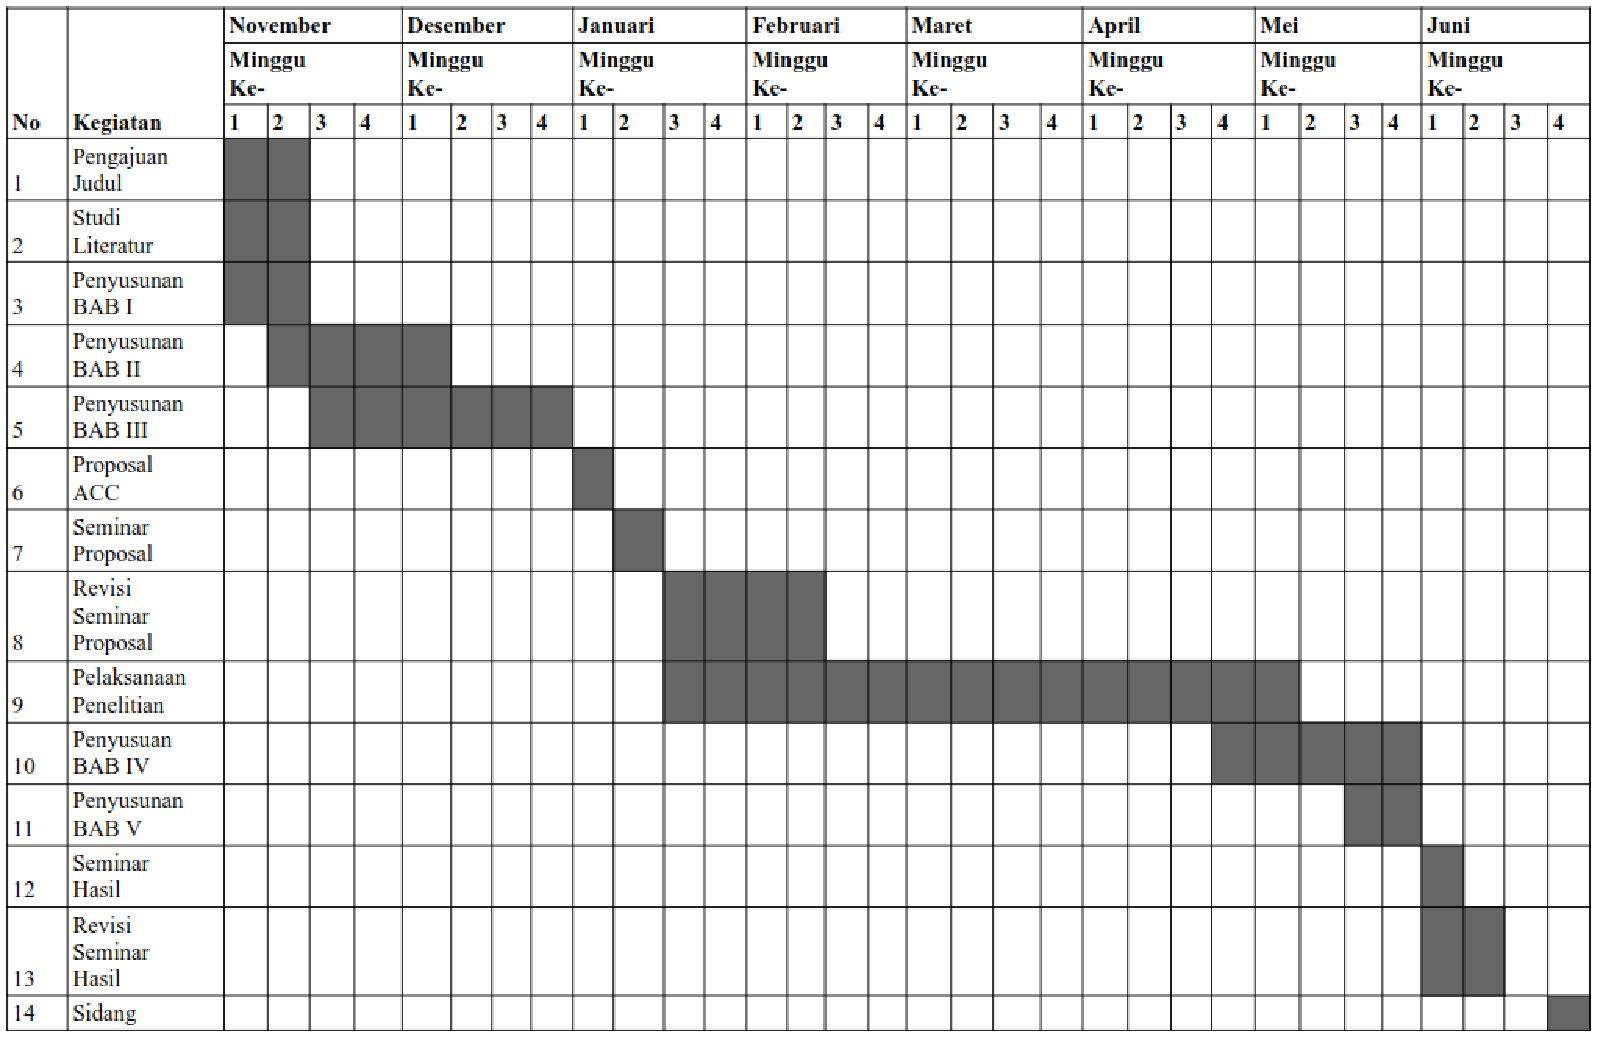
\includegraphics[width=\textwidth]{image/bab3/jadwal-pelaksanaan.pdf}\label{tab:jadwal_pelaksanaan}
% \end{table}


% Please add the following required packages to your document preamble:
% \usepackage{multirow}
% \usepackage{graphicx}
% \usepackage[table,xcdraw]{xcolor}
% Beamer presentation requires \usepackage{colortbl} instead of \usepackage[table,xcdraw]{xcolor}
\begin{table}[H]
  \centering
  \caption{Jadwal pelaksanaan penelitian}
  \label{tab:jadwal_pelaksanaan}
  \resizebox{\textwidth}{!}{%
  \begin{tabular}{|l|l|llllllllllllllllllllllll|}
  \hline
   &
     &
    \multicolumn{24}{c|}{\textbf{Bulan Ke -}} \\ \cline{3-26} 
   &
     &
    \multicolumn{4}{c|}{\textbf{Januari}} &
    \multicolumn{4}{c|}{\textbf{Februari}} &
    \multicolumn{4}{c|}{\textbf{Maret}} &
    \multicolumn{4}{c|}{\textbf{April}} &
    \multicolumn{4}{c|}{\textbf{Mei}} &
    \multicolumn{4}{c|}{\textbf{Juni}} \\ \cline{3-26} 
  \multirow{-3}{*}{\textbf{No}} &
    \multirow{-3}{*}{\textbf{Kegiatan}} &
    \multicolumn{1}{c|}{\textbf{1}} &
    \multicolumn{1}{c|}{\textbf{2}} &
    \multicolumn{1}{c|}{\textbf{3}} &
    \multicolumn{1}{c|}{\textbf{4}} &
    \multicolumn{1}{c|}{\textbf{1}} &
    \multicolumn{1}{c|}{\textbf{2}} &
    \multicolumn{1}{c|}{\textbf{3}} &
    \multicolumn{1}{c|}{\textbf{4}} &
    \multicolumn{1}{c|}{\textbf{1}} &
    \multicolumn{1}{c|}{\textbf{2}} &
    \multicolumn{1}{c|}{\textbf{3}} &
    \multicolumn{1}{c|}{\textbf{4}} &
    \multicolumn{1}{c|}{\textbf{1}} &
    \multicolumn{1}{c|}{\textbf{2}} &
    \multicolumn{1}{c|}{\textbf{3}} &
    \multicolumn{1}{c|}{\textbf{4}} &
    \multicolumn{1}{c|}{\textbf{1}} &
    \multicolumn{1}{c|}{\textbf{2}} &
    \multicolumn{1}{c|}{\textbf{3}} &
    \multicolumn{1}{c|}{\textbf{4}} &
    \multicolumn{1}{c|}{\textbf{1}} &
    \multicolumn{1}{c|}{\textbf{2}} &
    \multicolumn{1}{c|}{\textbf{3}} &
    \multicolumn{1}{c|}{\textbf{4}} \\ \hline
  1 &
    Studi literatur &
    \multicolumn{1}{l|}{\cellcolor[HTML]{333333}{\color[HTML]{333333} }} &
    \multicolumn{1}{l|}{\cellcolor[HTML]{333333}{\color[HTML]{333333} }} &
    \multicolumn{1}{l|}{\cellcolor[HTML]{333333}{\color[HTML]{333333} }} &
    \multicolumn{1}{l|}{\cellcolor[HTML]{333333}{\color[HTML]{333333} }} &
    \multicolumn{1}{l|}{} &
    \multicolumn{1}{l|}{} &
    \multicolumn{1}{l|}{} &
    \multicolumn{1}{l|}{} &
    \multicolumn{1}{l|}{} &
    \multicolumn{1}{l|}{} &
    \multicolumn{1}{l|}{} &
    \multicolumn{1}{l|}{} &
    \multicolumn{1}{l|}{} &
    \multicolumn{1}{l|}{} &
    \multicolumn{1}{l|}{} &
    \multicolumn{1}{l|}{} &
    \multicolumn{1}{l|}{} &
    \multicolumn{1}{l|}{} &
    \multicolumn{1}{l|}{} &
    \multicolumn{1}{l|}{} &
    \multicolumn{1}{l|}{} &
    \multicolumn{1}{l|}{} &
    \multicolumn{1}{l|}{} &
     \\ \hline
  2 &
    Pengumpulan data &
    \multicolumn{1}{l|}{} &
    \multicolumn{1}{l|}{} &
    \multicolumn{1}{l|}{\cellcolor[HTML]{333333}} &
    \multicolumn{1}{l|}{\cellcolor[HTML]{333333}} &
    \multicolumn{1}{l|}{\cellcolor[HTML]{333333}} &
    \multicolumn{1}{l|}{\cellcolor[HTML]{333333}} &
    \multicolumn{1}{l|}{} &
    \multicolumn{1}{l|}{} &
    \multicolumn{1}{l|}{} &
    \multicolumn{1}{l|}{} &
    \multicolumn{1}{l|}{} &
    \multicolumn{1}{l|}{} &
    \multicolumn{1}{l|}{} &
    \multicolumn{1}{l|}{} &
    \multicolumn{1}{l|}{} &
    \multicolumn{1}{l|}{} &
    \multicolumn{1}{l|}{} &
    \multicolumn{1}{l|}{} &
    \multicolumn{1}{l|}{} &
    \multicolumn{1}{l|}{} &
    \multicolumn{1}{l|}{} &
    \multicolumn{1}{l|}{} &
    \multicolumn{1}{l|}{} &
     \\ \hline
  3 &
    Pemrosesan data &
    \multicolumn{1}{l|}{} &
    \multicolumn{1}{l|}{} &
    \multicolumn{1}{l|}{} &
    \multicolumn{1}{l|}{} &
    \multicolumn{1}{l|}{\cellcolor[HTML]{333333}} &
    \multicolumn{1}{l|}{\cellcolor[HTML]{333333}} &
    \multicolumn{1}{l|}{\cellcolor[HTML]{333333}} &
    \multicolumn{1}{l|}{\cellcolor[HTML]{333333}} &
    \multicolumn{1}{l|}{\cellcolor[HTML]{333333}} &
    \multicolumn{1}{l|}{\cellcolor[HTML]{333333}} &
    \multicolumn{1}{l|}{} &
    \multicolumn{1}{l|}{} &
    \multicolumn{1}{l|}{} &
    \multicolumn{1}{l|}{} &
    \multicolumn{1}{l|}{} &
    \multicolumn{1}{l|}{} &
    \multicolumn{1}{l|}{} &
    \multicolumn{1}{l|}{} &
    \multicolumn{1}{l|}{} &
    \multicolumn{1}{l|}{} &
    \multicolumn{1}{l|}{} &
    \multicolumn{1}{l|}{} &
    \multicolumn{1}{l|}{} &
     \\ \hline
  4 &
    Membangun model &
    \multicolumn{1}{l|}{} &
    \multicolumn{1}{l|}{} &
    \multicolumn{1}{l|}{} &
    \multicolumn{1}{l|}{} &
    \multicolumn{1}{l|}{} &
    \multicolumn{1}{l|}{} &
    \multicolumn{1}{l|}{} &
    \multicolumn{1}{l|}{} &
    \multicolumn{1}{l|}{} &
    \multicolumn{1}{l|}{} &
    \multicolumn{1}{l|}{\cellcolor[HTML]{333333}} &
    \multicolumn{1}{l|}{\cellcolor[HTML]{333333}} &
    \multicolumn{1}{l|}{} &
    \multicolumn{1}{l|}{} &
    \multicolumn{1}{l|}{} &
    \multicolumn{1}{l|}{} &
    \multicolumn{1}{l|}{} &
    \multicolumn{1}{l|}{} &
    \multicolumn{1}{l|}{} &
    \multicolumn{1}{l|}{} &
    \multicolumn{1}{l|}{} &
    \multicolumn{1}{l|}{} &
    \multicolumn{1}{l|}{} &
     \\ \hline
  5 &
    Melatih model &
    \multicolumn{1}{l|}{} &
    \multicolumn{1}{l|}{} &
    \multicolumn{1}{l|}{} &
    \multicolumn{1}{l|}{} &
    \multicolumn{1}{l|}{} &
    \multicolumn{1}{l|}{} &
    \multicolumn{1}{l|}{} &
    \multicolumn{1}{l|}{} &
    \multicolumn{1}{l|}{} &
    \multicolumn{1}{l|}{} &
    \multicolumn{1}{l|}{} &
    \multicolumn{1}{l|}{\cellcolor[HTML]{333333}} &
    \multicolumn{1}{l|}{\cellcolor[HTML]{333333}} &
    \multicolumn{1}{l|}{\cellcolor[HTML]{333333}} &
    \multicolumn{1}{l|}{\cellcolor[HTML]{333333}} &
    \multicolumn{1}{l|}{\cellcolor[HTML]{333333}} &
    \multicolumn{1}{l|}{\cellcolor[HTML]{333333}} &
    \multicolumn{1}{l|}{\cellcolor[HTML]{333333}} &
    \multicolumn{1}{l|}{} &
    \multicolumn{1}{l|}{} &
    \multicolumn{1}{l|}{} &
    \multicolumn{1}{l|}{} &
    \multicolumn{1}{l|}{} &
     \\ \hline
  6 &
    Analisis hasil &
    \multicolumn{1}{l|}{} &
    \multicolumn{1}{l|}{} &
    \multicolumn{1}{l|}{} &
    \multicolumn{1}{l|}{} &
    \multicolumn{1}{l|}{} &
    \multicolumn{1}{l|}{} &
    \multicolumn{1}{l|}{} &
    \multicolumn{1}{l|}{} &
    \multicolumn{1}{l|}{} &
    \multicolumn{1}{l|}{} &
    \multicolumn{1}{l|}{} &
    \multicolumn{1}{l|}{} &
    \multicolumn{1}{l|}{} &
    \multicolumn{1}{l|}{} &
    \multicolumn{1}{l|}{} &
    \multicolumn{1}{l|}{} &
    \multicolumn{1}{l|}{} &
    \multicolumn{1}{l|}{} &
    \multicolumn{1}{l|}{\cellcolor[HTML]{333333}} &
    \multicolumn{1}{l|}{} &
    \multicolumn{1}{l|}{} &
    \multicolumn{1}{l|}{} &
    \multicolumn{1}{l|}{} &
     \\ \hline
  7 &
    Penyusunan laporan akhir &
    \multicolumn{1}{l|}{} &
    \multicolumn{1}{l|}{} &
    \multicolumn{1}{l|}{} &
    \multicolumn{1}{l|}{} &
    \multicolumn{1}{l|}{} &
    \multicolumn{1}{l|}{} &
    \multicolumn{1}{l|}{} &
    \multicolumn{1}{l|}{} &
    \multicolumn{1}{l|}{} &
    \multicolumn{1}{l|}{} &
    \multicolumn{1}{l|}{} &
    \multicolumn{1}{l|}{} &
    \multicolumn{1}{l|}{} &
    \multicolumn{1}{l|}{} &
    \multicolumn{1}{l|}{} &
    \multicolumn{1}{l|}{} &
    \multicolumn{1}{l|}{} &
    \multicolumn{1}{l|}{} &
    \multicolumn{1}{l|}{} &
    \multicolumn{1}{l|}{\cellcolor[HTML]{333333}} &
    \multicolumn{1}{l|}{\cellcolor[HTML]{333333}} &
    \multicolumn{1}{l|}{\cellcolor[HTML]{333333}} &
    \multicolumn{1}{l|}{} &
     \\ \hline
  \end{tabular}%
  }
  \end{table}


% Please add the following required packages to your document preamble:
% \usepackage{multirow}
% \usepackage{graphicx}
% \usepackage[table,xcdraw]{xcolor}
% Beamer presentation requires \usepackage{colortbl} instead of \usepackage[table,xcdraw]{xcolor}
% \begin{table}[H]
%     \centering
%     \caption{Jadwal pelaksanaan penelitian}
%     \label{tab: jadwal-pelaksanaan}
%     \resizebox{\textwidth}{!}{%
%     \begin{tabular}{|l|l|llll|llll|llll|llll|llll|llll|llll|llll|}
%     \hline
%      &
%        &
%       \multicolumn{4}{l|}{\textbf{November}} &
%       \multicolumn{4}{l|}{\textbf{Desember}} &
%       \multicolumn{4}{l|}{\textbf{Januari}} &
%       \multicolumn{4}{l|}{\textbf{Februari}} &
%       \multicolumn{4}{l|}{\textbf{Maret}} &
%       \multicolumn{4}{l|}{\textbf{April}} &
%       \multicolumn{4}{l|}{\textbf{Mei}} &
%       \multicolumn{4}{l|}{\textbf{Juni}} \\ \cline{3-34} 
%      &
%        &
%       \multicolumn{4}{l|}{\textbf{\begin{tabular}[c]{@{}l@{}}Minggu\\ Ke-\end{tabular}}} &
%       \multicolumn{4}{l|}{\textbf{\begin{tabular}[c]{@{}l@{}}Minggu\\ Ke-\end{tabular}}} &
%       \multicolumn{4}{l|}{\textbf{\begin{tabular}[c]{@{}l@{}}Minggu\\ Ke-\end{tabular}}} &
%       \multicolumn{4}{l|}{\textbf{\begin{tabular}[c]{@{}l@{}}Minggu\\ Ke-\end{tabular}}} &
%       \multicolumn{4}{l|}{\textbf{\begin{tabular}[c]{@{}l@{}}Minggu\\ Ke-\end{tabular}}} &
%       \multicolumn{4}{l|}{\textbf{\begin{tabular}[c]{@{}l@{}}Minggu\\ Ke-\end{tabular}}} &
%       \multicolumn{4}{l|}{\textbf{\begin{tabular}[c]{@{}l@{}}Minggu\\ Ke-\end{tabular}}} &
%       \multicolumn{4}{l|}{\textbf{\begin{tabular}[c]{@{}l@{}}Minggu\\ Ke-\end{tabular}}} \\ \cline{3-34} 
%     \multirow{-3}{*}{\textbf{No}} &
%       \multirow{-3}{*}{\textbf{Kegiatan}} &
%       \multicolumn{1}{l|}{\textbf{1}} &
%       \multicolumn{1}{l|}{\textbf{2}} &
%       \multicolumn{1}{l|}{\textbf{3}} &
%       \textbf{4} &
%       \multicolumn{1}{l|}{\textbf{1}} &
%       \multicolumn{1}{l|}{\textbf{2}} &
%       \multicolumn{1}{l|}{\textbf{3}} &
%       \textbf{4} &
%       \multicolumn{1}{l|}{\textbf{1}} &
%       \multicolumn{1}{l|}{\textbf{2}} &
%       \multicolumn{1}{l|}{\textbf{3}} &
%       \textbf{4} &
%       \multicolumn{1}{l|}{\textbf{1}} &
%       \multicolumn{1}{l|}{\textbf{2}} &
%       \multicolumn{1}{l|}{\textbf{3}} &
%       \textbf{4} &
%       \multicolumn{1}{l|}{\textbf{1}} &
%       \multicolumn{1}{l|}{\textbf{2}} &
%       \multicolumn{1}{l|}{\textbf{3}} &
%       \textbf{4} &
%       \multicolumn{1}{l|}{\textbf{1}} &
%       \multicolumn{1}{l|}{\textbf{2}} &
%       \multicolumn{1}{l|}{\textbf{3}} &
%       \textbf{4} &
%       \multicolumn{1}{l|}{\textbf{1}} &
%       \multicolumn{1}{l|}{\textbf{2}} &
%       \multicolumn{1}{l|}{\textbf{3}} &
%       \textbf{4} &
%       \multicolumn{1}{l|}{\textbf{1}} &
%       \multicolumn{1}{l|}{\textbf{2}} &
%       \multicolumn{1}{l|}{\textbf{3}} &
%       \textbf{4} \\ \hline
%     1 &
%       \begin{tabular}[c]{@{}l@{}}Pengajuan \\ Judul\end{tabular} &
%       \multicolumn{1}{l|}{\cellcolor[HTML]{666666}} &
%       \multicolumn{1}{l|}{\cellcolor[HTML]{666666}} &
%       \multicolumn{1}{l|}{} &
%        &
%       \multicolumn{1}{l|}{} &
%       \multicolumn{1}{l|}{} &
%       \multicolumn{1}{l|}{} &
%        &
%       \multicolumn{1}{l|}{} &
%       \multicolumn{1}{l|}{} &
%       \multicolumn{1}{l|}{} &
%        &
%       \multicolumn{1}{l|}{} &
%       \multicolumn{1}{l|}{} &
%       \multicolumn{1}{l|}{} &
%        &
%       \multicolumn{1}{l|}{} &
%       \multicolumn{1}{l|}{} &
%       \multicolumn{1}{l|}{} &
%        &
%       \multicolumn{1}{l|}{} &
%       \multicolumn{1}{l|}{} &
%       \multicolumn{1}{l|}{} &
%        &
%       \multicolumn{1}{l|}{} &
%       \multicolumn{1}{l|}{} &
%       \multicolumn{1}{l|}{} &
%        &
%       \multicolumn{1}{l|}{} &
%       \multicolumn{1}{l|}{} &
%       \multicolumn{1}{l|}{} &
%        \\ \hline
%     2 &
%       \begin{tabular}[c]{@{}l@{}}Studi \\ Literatur\end{tabular} &
%       \multicolumn{1}{l|}{\cellcolor[HTML]{666666}} &
%       \multicolumn{1}{l|}{\cellcolor[HTML]{666666}} &
%       \multicolumn{1}{l|}{} &
%        &
%       \multicolumn{1}{l|}{} &
%       \multicolumn{1}{l|}{} &
%       \multicolumn{1}{l|}{} &
%        &
%       \multicolumn{1}{l|}{} &
%       \multicolumn{1}{l|}{} &
%       \multicolumn{1}{l|}{} &
%        &
%       \multicolumn{1}{l|}{} &
%       \multicolumn{1}{l|}{} &
%       \multicolumn{1}{l|}{} &
%        &
%       \multicolumn{1}{l|}{} &
%       \multicolumn{1}{l|}{} &
%       \multicolumn{1}{l|}{} &
%        &
%       \multicolumn{1}{l|}{} &
%       \multicolumn{1}{l|}{} &
%       \multicolumn{1}{l|}{} &
%        &
%       \multicolumn{1}{l|}{} &
%       \multicolumn{1}{l|}{} &
%       \multicolumn{1}{l|}{} &
%        &
%       \multicolumn{1}{l|}{} &
%       \multicolumn{1}{l|}{} &
%       \multicolumn{1}{l|}{} &
%        \\ \hline
%     3 &
%       \begin{tabular}[c]{@{}l@{}}Penyusunan \\ BAB I\end{tabular} &
%       \multicolumn{1}{l|}{\cellcolor[HTML]{666666}} &
%       \multicolumn{1}{l|}{\cellcolor[HTML]{666666}} &
%       \multicolumn{1}{l|}{} &
%        &
%       \multicolumn{1}{l|}{} &
%       \multicolumn{1}{l|}{} &
%       \multicolumn{1}{l|}{} &
%        &
%       \multicolumn{1}{l|}{} &
%       \multicolumn{1}{l|}{} &
%       \multicolumn{1}{l|}{} &
%        &
%       \multicolumn{1}{l|}{} &
%       \multicolumn{1}{l|}{} &
%       \multicolumn{1}{l|}{} &
%        &
%       \multicolumn{1}{l|}{} &
%       \multicolumn{1}{l|}{} &
%       \multicolumn{1}{l|}{} &
%        &
%       \multicolumn{1}{l|}{} &
%       \multicolumn{1}{l|}{} &
%       \multicolumn{1}{l|}{} &
%        &
%       \multicolumn{1}{l|}{} &
%       \multicolumn{1}{l|}{} &
%       \multicolumn{1}{l|}{} &
%        &
%       \multicolumn{1}{l|}{} &
%       \multicolumn{1}{l|}{} &
%       \multicolumn{1}{l|}{} &
%        \\ \hline
%     4 &
%       \begin{tabular}[c]{@{}l@{}}Penyusunan \\ BAB II\end{tabular} &
%       \multicolumn{1}{l|}{} &
%       \multicolumn{1}{l|}{\cellcolor[HTML]{666666}} &
%       \multicolumn{1}{l|}{\cellcolor[HTML]{666666}} &
%       \cellcolor[HTML]{666666} &
%       \multicolumn{1}{l|}{\cellcolor[HTML]{666666}} &
%       \multicolumn{1}{l|}{} &
%       \multicolumn{1}{l|}{} &
%        &
%       \multicolumn{1}{l|}{} &
%       \multicolumn{1}{l|}{} &
%       \multicolumn{1}{l|}{} &
%        &
%       \multicolumn{1}{l|}{} &
%       \multicolumn{1}{l|}{} &
%       \multicolumn{1}{l|}{} &
%        &
%       \multicolumn{1}{l|}{} &
%       \multicolumn{1}{l|}{} &
%       \multicolumn{1}{l|}{} &
%        &
%       \multicolumn{1}{l|}{} &
%       \multicolumn{1}{l|}{} &
%       \multicolumn{1}{l|}{} &
%        &
%       \multicolumn{1}{l|}{} &
%       \multicolumn{1}{l|}{} &
%       \multicolumn{1}{l|}{} &
%        &
%       \multicolumn{1}{l|}{} &
%       \multicolumn{1}{l|}{} &
%       \multicolumn{1}{l|}{} &
%        \\ \hline
%     5 &
%       \begin{tabular}[c]{@{}l@{}}Penyusunan \\ BAB III\end{tabular} &
%       \multicolumn{1}{l|}{} &
%       \multicolumn{1}{l|}{} &
%       \multicolumn{1}{l|}{\cellcolor[HTML]{666666}} &
%       \cellcolor[HTML]{666666} &
%       \multicolumn{1}{l|}{\cellcolor[HTML]{666666}} &
%       \multicolumn{1}{l|}{\cellcolor[HTML]{666666}} &
%       \multicolumn{1}{l|}{\cellcolor[HTML]{666666}} &
%       \cellcolor[HTML]{666666} &
%       \multicolumn{1}{l|}{} &
%       \multicolumn{1}{l|}{} &
%       \multicolumn{1}{l|}{} &
%        &
%       \multicolumn{1}{l|}{} &
%       \multicolumn{1}{l|}{} &
%       \multicolumn{1}{l|}{} &
%        &
%       \multicolumn{1}{l|}{} &
%       \multicolumn{1}{l|}{} &
%       \multicolumn{1}{l|}{} &
%        &
%       \multicolumn{1}{l|}{} &
%       \multicolumn{1}{l|}{} &
%       \multicolumn{1}{l|}{} &
%        &
%       \multicolumn{1}{l|}{} &
%       \multicolumn{1}{l|}{} &
%       \multicolumn{1}{l|}{} &
%        &
%       \multicolumn{1}{l|}{} &
%       \multicolumn{1}{l|}{} &
%       \multicolumn{1}{l|}{} &
%        \\ \hline
%     6 &
%       \begin{tabular}[c]{@{}l@{}}Proposal \\ ACC\end{tabular} &
%       \multicolumn{1}{l|}{} &
%       \multicolumn{1}{l|}{} &
%       \multicolumn{1}{l|}{} &
%        &
%       \multicolumn{1}{l|}{} &
%       \multicolumn{1}{l|}{} &
%       \multicolumn{1}{l|}{} &
%        &
%       \multicolumn{1}{l|}{\cellcolor[HTML]{666666}} &
%       \multicolumn{1}{l|}{} &
%       \multicolumn{1}{l|}{} &
%        &
%       \multicolumn{1}{l|}{} &
%       \multicolumn{1}{l|}{} &
%       \multicolumn{1}{l|}{} &
%        &
%       \multicolumn{1}{l|}{} &
%       \multicolumn{1}{l|}{} &
%       \multicolumn{1}{l|}{} &
%        &
%       \multicolumn{1}{l|}{} &
%       \multicolumn{1}{l|}{} &
%       \multicolumn{1}{l|}{} &
%        &
%       \multicolumn{1}{l|}{} &
%       \multicolumn{1}{l|}{} &
%       \multicolumn{1}{l|}{} &
%        &
%       \multicolumn{1}{l|}{} &
%       \multicolumn{1}{l|}{} &
%       \multicolumn{1}{l|}{} &
%        \\ \hline
%     7 &
%       \begin{tabular}[c]{@{}l@{}}Seminar \\ Proposal\end{tabular} &
%       \multicolumn{1}{l|}{} &
%       \multicolumn{1}{l|}{} &
%       \multicolumn{1}{l|}{} &
%        &
%       \multicolumn{1}{l|}{} &
%       \multicolumn{1}{l|}{} &
%       \multicolumn{1}{l|}{} &
%        &
%       \multicolumn{1}{l|}{} &
%       \multicolumn{1}{l|}{\cellcolor[HTML]{666666}} &
%       \multicolumn{1}{l|}{} &
%        &
%       \multicolumn{1}{l|}{} &
%       \multicolumn{1}{l|}{} &
%       \multicolumn{1}{l|}{} &
%        &
%       \multicolumn{1}{l|}{} &
%       \multicolumn{1}{l|}{} &
%       \multicolumn{1}{l|}{} &
%        &
%       \multicolumn{1}{l|}{} &
%       \multicolumn{1}{l|}{} &
%       \multicolumn{1}{l|}{} &
%        &
%       \multicolumn{1}{l|}{} &
%       \multicolumn{1}{l|}{} &
%       \multicolumn{1}{l|}{} &
%        &
%       \multicolumn{1}{l|}{} &
%       \multicolumn{1}{l|}{} &
%       \multicolumn{1}{l|}{} &
%        \\ \hline
%     8 &
%       \begin{tabular}[c]{@{}l@{}}Revisi \\ Seminar \\ Proposal\end{tabular} &
%       \multicolumn{1}{l|}{} &
%       \multicolumn{1}{l|}{} &
%       \multicolumn{1}{l|}{} &
%        &
%       \multicolumn{1}{l|}{} &
%       \multicolumn{1}{l|}{} &
%       \multicolumn{1}{l|}{} &
%        &
%       \multicolumn{1}{l|}{} &
%       \multicolumn{1}{l|}{} &
%       \multicolumn{1}{l|}{\cellcolor[HTML]{666666}} &
%       \cellcolor[HTML]{666666} &
%       \multicolumn{1}{l|}{\cellcolor[HTML]{666666}} &
%       \multicolumn{1}{l|}{\cellcolor[HTML]{666666}} &
%       \multicolumn{1}{l|}{} &
%        &
%       \multicolumn{1}{l|}{} &
%       \multicolumn{1}{l|}{} &
%       \multicolumn{1}{l|}{} &
%        &
%       \multicolumn{1}{l|}{} &
%       \multicolumn{1}{l|}{} &
%       \multicolumn{1}{l|}{} &
%        &
%       \multicolumn{1}{l|}{} &
%       \multicolumn{1}{l|}{} &
%       \multicolumn{1}{l|}{} &
%        &
%       \multicolumn{1}{l|}{} &
%       \multicolumn{1}{l|}{} &
%       \multicolumn{1}{l|}{} &
%        \\ \hline
%     9 &
%       \begin{tabular}[c]{@{}l@{}}Pelaksanaan \\ Penelitian\end{tabular} &
%       \multicolumn{1}{l|}{} &
%       \multicolumn{1}{l|}{} &
%       \multicolumn{1}{l|}{} &
%        &
%       \multicolumn{1}{l|}{} &
%       \multicolumn{1}{l|}{} &
%       \multicolumn{1}{l|}{} &
%        &
%       \multicolumn{1}{l|}{} &
%       \multicolumn{1}{l|}{} &
%       \multicolumn{1}{l|}{\cellcolor[HTML]{666666}} &
%       \cellcolor[HTML]{666666} &
%       \multicolumn{1}{l|}{\cellcolor[HTML]{666666}} &
%       \multicolumn{1}{l|}{\cellcolor[HTML]{666666}} &
%       \multicolumn{1}{l|}{\cellcolor[HTML]{666666}} &
%       \cellcolor[HTML]{666666} &
%       \multicolumn{1}{l|}{\cellcolor[HTML]{666666}} &
%       \multicolumn{1}{l|}{\cellcolor[HTML]{666666}} &
%       \multicolumn{1}{l|}{\cellcolor[HTML]{666666}} &
%       \cellcolor[HTML]{666666} &
%       \multicolumn{1}{l|}{\cellcolor[HTML]{666666}} &
%       \multicolumn{1}{l|}{\cellcolor[HTML]{666666}} &
%       \multicolumn{1}{l|}{\cellcolor[HTML]{666666}} &
%       \cellcolor[HTML]{666666} &
%       \multicolumn{1}{l|}{\cellcolor[HTML]{666666}} &
%       \multicolumn{1}{l|}{} &
%       \multicolumn{1}{l|}{} &
%        &
%       \multicolumn{1}{l|}{} &
%       \multicolumn{1}{l|}{} &
%       \multicolumn{1}{l|}{} &
%        \\ \hline
%     10 &
%       \begin{tabular}[c]{@{}l@{}}Penyusuan \\ BAB IV\end{tabular} &
%       \multicolumn{1}{l|}{} &
%       \multicolumn{1}{l|}{} &
%       \multicolumn{1}{l|}{} &
%        &
%       \multicolumn{1}{l|}{} &
%       \multicolumn{1}{l|}{} &
%       \multicolumn{1}{l|}{} &
%        &
%       \multicolumn{1}{l|}{} &
%       \multicolumn{1}{l|}{} &
%       \multicolumn{1}{l|}{} &
%        &
%       \multicolumn{1}{l|}{} &
%       \multicolumn{1}{l|}{} &
%       \multicolumn{1}{l|}{} &
%        &
%       \multicolumn{1}{l|}{} &
%       \multicolumn{1}{l|}{} &
%       \multicolumn{1}{l|}{} &
%        &
%       \multicolumn{1}{l|}{} &
%       \multicolumn{1}{l|}{} &
%       \multicolumn{1}{l|}{} &
%       \cellcolor[HTML]{666666} &
%       \multicolumn{1}{l|}{\cellcolor[HTML]{666666}} &
%       \multicolumn{1}{l|}{\cellcolor[HTML]{666666}} &
%       \multicolumn{1}{l|}{\cellcolor[HTML]{666666}} &
%       \cellcolor[HTML]{666666} &
%       \multicolumn{1}{l|}{} &
%       \multicolumn{1}{l|}{} &
%       \multicolumn{1}{l|}{} &
%        \\ \hline
%     11 &
%       \begin{tabular}[c]{@{}l@{}}Penyusunan \\ BAB V\end{tabular} &
%       \multicolumn{1}{l|}{} &
%       \multicolumn{1}{l|}{} &
%       \multicolumn{1}{l|}{} &
%        &
%       \multicolumn{1}{l|}{} &
%       \multicolumn{1}{l|}{} &
%       \multicolumn{1}{l|}{} &
%        &
%       \multicolumn{1}{l|}{} &
%       \multicolumn{1}{l|}{} &
%       \multicolumn{1}{l|}{} &
%        &
%       \multicolumn{1}{l|}{} &
%       \multicolumn{1}{l|}{} &
%       \multicolumn{1}{l|}{} &
%        &
%       \multicolumn{1}{l|}{} &
%       \multicolumn{1}{l|}{} &
%       \multicolumn{1}{l|}{} &
%        &
%       \multicolumn{1}{l|}{} &
%       \multicolumn{1}{l|}{} &
%       \multicolumn{1}{l|}{} &
%        &
%       \multicolumn{1}{l|}{} &
%       \multicolumn{1}{l|}{} &
%       \multicolumn{1}{l|}{\cellcolor[HTML]{666666}} &
%       \cellcolor[HTML]{666666} &
%       \multicolumn{1}{l|}{} &
%       \multicolumn{1}{l|}{} &
%       \multicolumn{1}{l|}{} &
%        \\ \hline
%     12 &
%       \begin{tabular}[c]{@{}l@{}}Seminar\\ Hasil\end{tabular} &
%       \multicolumn{1}{l|}{} &
%       \multicolumn{1}{l|}{} &
%       \multicolumn{1}{l|}{} &
%        &
%       \multicolumn{1}{l|}{} &
%       \multicolumn{1}{l|}{} &
%       \multicolumn{1}{l|}{} &
%        &
%       \multicolumn{1}{l|}{} &
%       \multicolumn{1}{l|}{} &
%       \multicolumn{1}{l|}{} &
%        &
%       \multicolumn{1}{l|}{} &
%       \multicolumn{1}{l|}{} &
%       \multicolumn{1}{l|}{} &
%        &
%       \multicolumn{1}{l|}{} &
%       \multicolumn{1}{l|}{} &
%       \multicolumn{1}{l|}{} &
%        &
%       \multicolumn{1}{l|}{} &
%       \multicolumn{1}{l|}{} &
%       \multicolumn{1}{l|}{} &
%        &
%       \multicolumn{1}{l|}{} &
%       \multicolumn{1}{l|}{} &
%       \multicolumn{1}{l|}{} &
%        &
%       \multicolumn{1}{l|}{\cellcolor[HTML]{666666}} &
%       \multicolumn{1}{l|}{} &
%       \multicolumn{1}{l|}{} &
%        \\ \hline
%     13 &
%       \begin{tabular}[c]{@{}l@{}}Revisi \\ Seminar \\ Hasil\end{tabular} &
%       \multicolumn{1}{l|}{} &
%       \multicolumn{1}{l|}{} &
%       \multicolumn{1}{l|}{} &
%        &
%       \multicolumn{1}{l|}{} &
%       \multicolumn{1}{l|}{} &
%       \multicolumn{1}{l|}{} &
%        &
%       \multicolumn{1}{l|}{} &
%       \multicolumn{1}{l|}{} &
%       \multicolumn{1}{l|}{} &
%        &
%       \multicolumn{1}{l|}{} &
%       \multicolumn{1}{l|}{} &
%       \multicolumn{1}{l|}{} &
%        &
%       \multicolumn{1}{l|}{} &
%       \multicolumn{1}{l|}{} &
%       \multicolumn{1}{l|}{} &
%        &
%       \multicolumn{1}{l|}{} &
%       \multicolumn{1}{l|}{} &
%       \multicolumn{1}{l|}{} &
%        &
%       \multicolumn{1}{l|}{} &
%       \multicolumn{1}{l|}{} &
%       \multicolumn{1}{l|}{} &
%        &
%       \multicolumn{1}{l|}{\cellcolor[HTML]{666666}} &
%       \multicolumn{1}{l|}{\cellcolor[HTML]{666666}} &
%       \multicolumn{1}{l|}{} &
%        \\ \hline
%     14 &
%       Sidang &
%       \multicolumn{1}{l|}{} &
%       \multicolumn{1}{l|}{} &
%       \multicolumn{1}{l|}{} &
%        &
%       \multicolumn{1}{l|}{} &
%       \multicolumn{1}{l|}{} &
%       \multicolumn{1}{l|}{} &
%        &
%       \multicolumn{1}{l|}{} &
%       \multicolumn{1}{l|}{} &
%       \multicolumn{1}{l|}{} &
%        &
%       \multicolumn{1}{l|}{} &
%       \multicolumn{1}{l|}{} &
%       \multicolumn{1}{l|}{} &
%        &
%       \multicolumn{1}{l|}{} &
%       \multicolumn{1}{l|}{} &
%       \multicolumn{1}{l|}{} &
%        &
%       \multicolumn{1}{l|}{} &
%       \multicolumn{1}{l|}{} &
%       \multicolumn{1}{l|}{} &
%        &
%       \multicolumn{1}{l|}{} &
%       \multicolumn{1}{l|}{} &
%       \multicolumn{1}{l|}{} &
%        &
%       \multicolumn{1}{l|}{} &
%       \multicolumn{1}{l|}{} &
%       \multicolumn{1}{l|}{} &
%       \cellcolor[HTML]{666666} \\ \hline
%     \end{tabular}%
%     }
% \end{table}

\section{Alat dan Bahan}
Alat dan Bahan yang akan digunakan pada penelitian ini terdiri dari beberapa perangkat keras (\textit{hardware}) dan perangkat lunak. Lalu, data yang digunakan adalah data dari \textit{\textit{dataset}} PathVQA, dan VQA-RAD. 

\subsection{Perangkat Keras}

\begin{enumerate}
	\item[a.] Laptop Lenovo Yoga C740 dengan RAM 16GB DDR4, Intel® Core™ i7-10710U. 1.10 - 4.70 GHz, \textit{Solid State State Drive} (SSD) 1TB.

    \item[b.] Server spesifikasi processor Intel Xeon Gold 5218, CPU 2.30GHz 64 inti, RAM 128GB, VGA 4 x NVIDIA GeForce RTX 2080 Ti GPU VRAM 12GB, dan memory 8TB.
\end{enumerate}

\subsection{Perangkat Lunak}
\begin{enumerate}
    \item[a.] Linux Debian Ubuntu versi 22.04 LTS
    \item[b.] Visual Studio Code versi 1.71.0
    \item[c.] Python versi 3.8.17
    \item[d.] PyTorch versi 2.0.1
    \item[e.] Tensorflow versi 2.11.0
    \item[f.] Transformers versi 4.31.0
    \item[g.] Huggingface Datasets versi 2.18.0
    \item[h.] FastAPI versi 0.104.1
    \item[i.] nlpaug versi 1.1.11
    

\end{enumerate}



\section{Metode Penelitian}

\par Penelitian ini akan mengikuti beberapa tahapan yang dirancang secara sistematis untuk mencapai tujuan yang telah ditetapkan. Setiap tahap akan dilaksanakan dengan seksama untuk memastikan hasil yang akurat dan bermanfaat. Skema dari alur tahapan penelitian yang diusulkan dapat dilihat secara rinci pada Gambar \ref{alur_penelitian}. Pada Gambar \ref{alur_penelitian} terdapat beberapa tahapan yang akan dilakukan dalam penelitian ini, yaitu identifikasi masalah, studi literatur, pengumpulan data, pemrosesan data, pembangunan model, pelatihan model, evaluasi model, dan pembangunan sistem medis cerdas berbasis web.

\begin{figure}[H]
\centering
{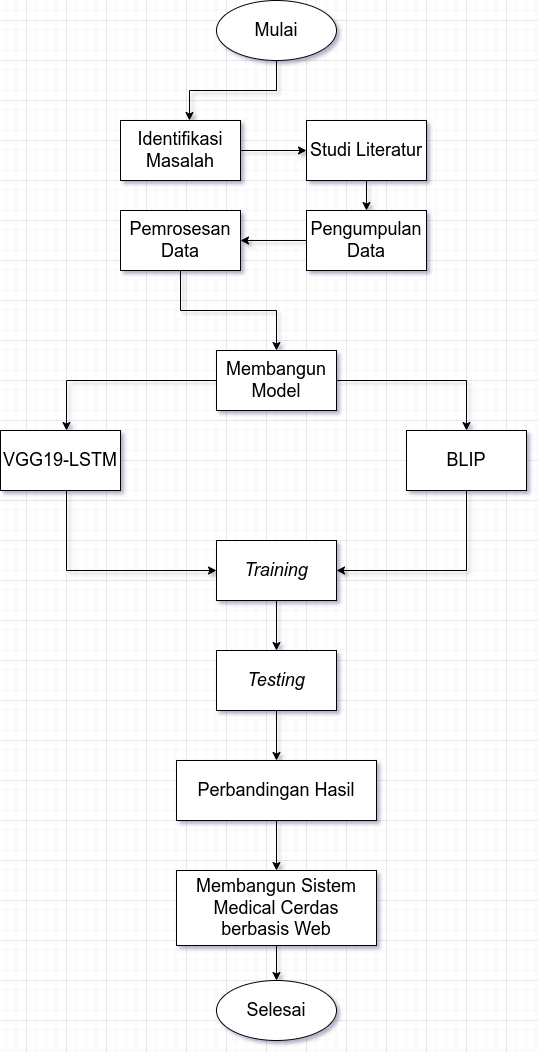
\includegraphics [width = 9cm, height= 16cm]{image/bab3/diagram_alir_penelitian8}}
\caption{Diagram alir penelitian}
\label{alur_penelitian}
\end{figure}

\subsection{Identifikasi Masalah}

\par Identifikasi masalah adalah proses awal dalam mengidentifikasi masalah yang akan diselesaikan dalam penelitian ini. Identifikasi masalah meliputi latar belakang masalah, rumusan masalah, tujuan penelitian serta manfaat yang dapat dihasilkan dari penelitian ini.

\subsection{Studi Literatur}

\par Studi literatur dilakukan untuk memperoleh informasi mengenai penelitian yang sudah dilakukan sebelumnya. Dalam tahapan ini terdiri dari banyak kegiatan yaitu membaca referensi yang berkaitan dengan penelitian ini, membaca jurnal atau buku untuk menambah wawasan, sehingga dapat memperoleh informasi yang dibutuhkan untuk penelitian ini.



\subsection{Pengumpulan Data}

\par Penelitian tugas akhir ini menggunakan data dari \textit{\textit{dataset}} PathVQA dan VQA-RAD. Pengumpulan \textit{\textit{dataset}} dilakukan dengan mengunduh data dari platform Hugging Face. Sampel kedua data ini bisa dilihat pada Gambar \ref{data_pathvqa} dan Gambar \ref{data_vqa-rad}.

\begin{figure}[H]
    \centering
    {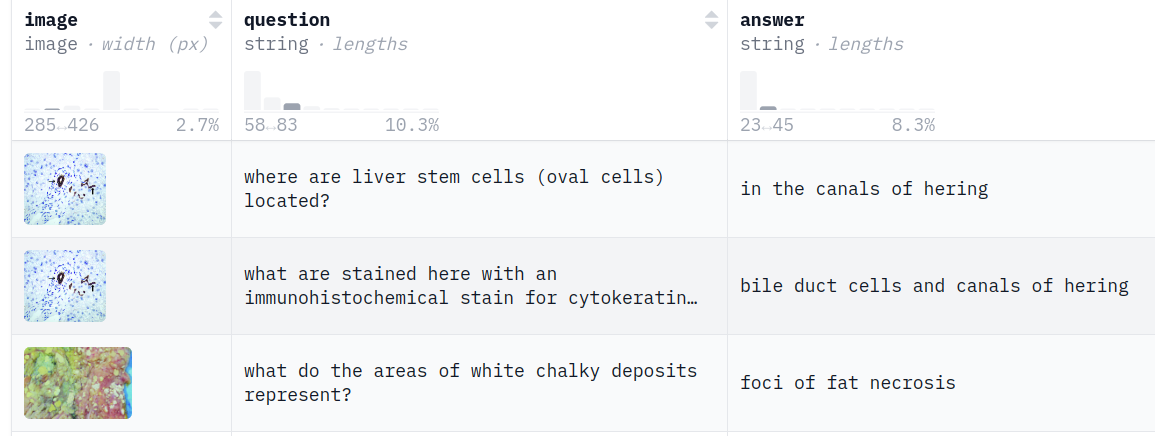
\includegraphics[width=\textwidth, height = 7cm]{image/bab3/pathvqa-sample.png}}
    \caption{Sampel data PathVQA}
    \label{data_pathvqa}
\end{figure}


\begin{figure}[H]
    \centering
    {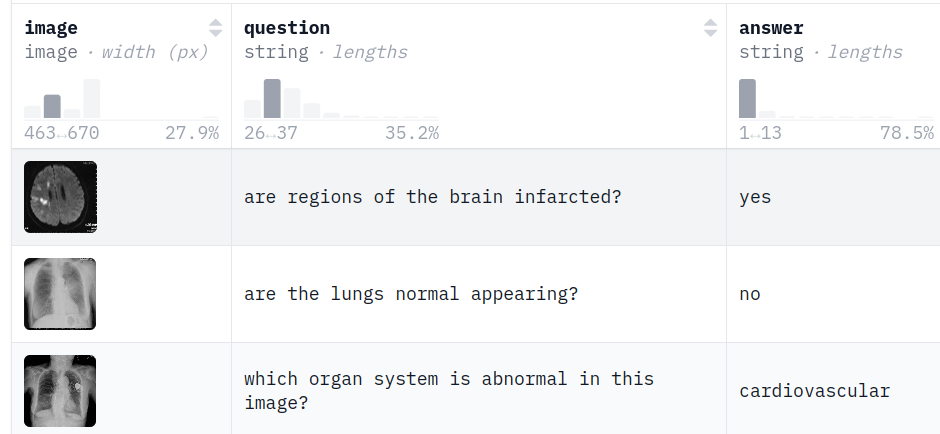
\includegraphics[width=\textwidth, height = 7cm]{image/bab3/vqarad-sample.png}}
    \caption{Sampel data VQA-RAD}
    \label{data_vqa-rad}
\end{figure}


\subsection{Pemrosesan Data}

\par Pada bagian ini, dilakukan pemrosesan data dengan tujuan menyelaraskan dan menyusun \textit{dataset} yang diperlukan untuk model \textit{Visual Question Answering} (VQA). Proses ini melibatkan penggabungan antara data visual, seperti gambar, dan data teks, berupa pertanyaan yang berkaitan. Pemrosesan data bertujuan untuk mengkonversi informasi kompleks dari kedua modalitas ini ke dalam format yang dapat dicerna oleh model. Dengan melakukan pemrosesan data ini, kita menciptakan representasi yang optimal untuk menyajikan informasi visual dan teks kepada model VQA. Hasilnya adalah \textit{dataset} yang kohesif dan siap digunakan untuk melatih model VQA agar mampu memberikan jawaban yang tepat terhadap pertanyaan yang diajukan berdasarkan konteks visual yang diberikan. Adapun pemrosesan data yang dilakukan mencakup pemrosesan gambar dan teks.


\begin{enumerate}

\item{\textit{Case Folding}}

\par Pada bagian ini proses \textit{case folding} dilakukan untuk mengubah semua karakter dalam teks menjadi huruf kecil. Hal ini dilakukan untuk menghindari duplikasi kata yang sama dengan huruf besar dan kecil. Tabel \ref{tab:case-folding} menunjukkan contoh proses \textit{case folding}.

\begin{table}[H]
    \centering
    \caption{Proses \textit{case folding}}
    \label{tab:case-folding}
    \begin{tabular}{|l|l|}
    \hline
    \multicolumn{1}{|c|}{\textbf{Sebelum}} & \multicolumn{1}{c|}{\textbf{Sesudah}} \\ \hline
    The Quick Brown Fox JUMPS              & the quick brown fox jumps             \\ \hline
    \end{tabular}
\end{table}


\item{\textit{Remove Punctuation}}

\par Pada bagian ini proses \textit{remove punctuation} dilakukan untuk menghapus tanda baca dalam teks. Hal ini dilakukan untuk mengurangi kompleksitas kata dalam teks. Tabel \ref{tab:remove-punctuation} menunjukkan contoh proses \textit{remove punctuation}.

\begin{table}[H]
    \centering
    \caption{Proses \textit{remove punctuation}}
    \label{tab:remove-punctuation}
    \begin{tabular}{|l|l|}
    \hline
    \multicolumn{1}{|c|}{\textbf{Sebelum}} & \multicolumn{1}{c|}{\textbf{Sesudah}} \\ \hline
    She said, 'Hello!' and waved           & She said Hello and waved              \\ \hline
    \end{tabular}
\end{table}

\item{\textit{Stemming}}

\par Pada bagian ini proses \textit{stemming} dilakukan untuk mengubah kata-kata dalam teks menjadi kata dasar. Hal ini dilakukan untuk mengurangi kompleksitas kata dalam teks. Tabel \ref{tab:stemming-text} menunjukkan contoh proses \textit{stemming-text}.

\begin{table}[H]
    \centering
    \caption{Proses \textit{stemming}}
    \label{tab:stemming-text}
    \begin{tabular}{|l|l|}
    \hline
    \multicolumn{1}{|c|}{\textbf{Sebelum}} & \multicolumn{1}{c|}{\textbf{Sesudah}} \\ \hline
    running quickly in the park            & run quick in the park                 \\ \hline
    \end{tabular}
\end{table}

\item{Tokenisasi}

\par Pada bagian ini proses tokenisasi dilakukan untuk memecah teks menjadi token-token yang lebih kecil. Hal ini dilakukan untuk mempermudah model VQA memahami dan memproses secara efektif. Tabel \ref{tab:tokenisasi} menunjukkan contoh proses tokenisasi.

\begin{table}[H]
    \centering
    \caption{Proses tokenisasi}
    \label{tab:tokenisasi}
    \begin{tabular}{|l|l|}
    \hline
    \multicolumn{1}{|c|}{\textbf{Sebelum}} & \multicolumn{1}{c|}{\textbf{Sesudah}}  \\ \hline
    The cat in the hat                     & {[}The, cat, in, the, hat{]} \\ \hline
    \end{tabular}
\end{table}

\item{Pemrosesan Gambar}

\par Pada bagian ini proses pemrosesan gambar dilakukan menyamaratakan format gambar. Hal ini dilakukan untuk mempermudah proses pemrosesan data dan mempersiapkan data agar siap digunakan untuk melatih model VQA.


\end{enumerate}

\subsection{Membangun Model}

\par Proses membangun model VQA ini menggunakan arsitektur VGG19-LSTM dan BLIP. Pada VGG19-LSTM, terdapat dua tahap pemrosesan, yaitu ekstraksi fitur gambar menggunakan VGG19 dan pemrosesan teks menggunakan LSTM. Sedangkan pada BLIP, terdapat dua \textit{encoder}, yaitu \textit{image encoder} dan \textit{text encoder}, yang digunakan untuk mengolah data gambar dan teks. Dalam BLIP, \textit{image encoder} menggunakan \textit{Vision Transformer} (ViT), sedangkan \textit{text encoder} menggunakan \textit{transformer encoder}. Proses ini bertujuan untuk membangun model VQA yang mampu memberikan jawaban yang tepat terhadap pertanyaan yang diberikan berdasarkan konteks visual yang diberikan.



\subsection{Melatih Model}

\par Tahapan pada pelatihan model ini menggunakan arsitektur VGG19-LSTM dan BLIP. Pada tahap ini akan dilakukan suatu metode yang bertujuan untuk mengubah nilai atau parameter yang ada pada suatu arsitektur, Proses ini disebut sebagai \textit{hyperparameter tuning}. \textit{Hyperparameter} ini mengacu pada parameter yang tidak dapat diubah ketika proses pelatihan model berjalan, contohnya seperti jumlah \textit{hidden layer}, nilai \textit{epoch}, \textit{batch size}, \textit{learning rate} pada fungsi optimasi, dan lain-lain. \textit{Hyperparameter tuning} ini dilakukan untuk mencari kombinasi nilai yang optimal untuk parameter-parameter tersebut \citep{yu2020hyper}.

\subsection{Perbandingan Hasil}

\par Setelah proses pelatihan model selesai, maka dilakukan perbandingan hasil dari kedua model yang telah dibangun dengan menggunakan metrik evaluasi yaitu akurasi dan \textit{Bilingual Evaluation Understudy} (BLEU). Pada metrik BLEU, penulis akan menggunakan BLEU-1, BLEU-2, dan BLEU-3, bilangan pada nama BLEU menunjukkan jumlah n-gram yang digunakan. Kedua metrik ini digunakan untuk mengevaluasi kinerja dari model VQA yang telah dilatih. Perbandingan hasil ini dilakukan dengan cara menguji kedua model menggunakan data uji yang telah disiapkan. Hasil dari perbandingan ini akan digunakan untuk menentukan model mana yang lebih baik dalam memberikan jawaban dari pertanyaan yang diberikan. 




\subsection{Membangun Sistem Medis Cerdas Berbasis Web}

\par Model yang telah siap dilatih akan di \textit{deploy} ke dalam sistem medis cerdas berbasis web. Dalam proses membangun \textit{website} ini meliputi pengembangan halaman tampilan yang bisa menerima dua \textit{input} yaitu gambar dan pertanyaan dari pengguna. Setelah itu mengembangkan bagian \textit{backend} untuk mengolah kedua \textit{input} tersebut dan memasukkannya ke dalam model yang telah dibangun sebelumnya. Setelah model menghasilkan jawaban, maka jawaban tersebut akan dikirimkan kembali ke halaman tampilan untuk ditampilkan kepada pengguna.




%-----------------------------------------------------------------------------%

% Baris ini digunakan untuk membantu dalam melakukan sitasi
% Karena diapit dengan comment, maka baris ini akan diabaikan
% oleh compiler LaTeX.
\begin{comment}
\bibliography{daftar-pustaka}
\end{comment}


\fancyhf{} 
\fancyfoot[R]{\thepage}

%-------------------------------------------------------------------------------
%                            BAB IV
%               		HASIL DAN PEMBAHASAN
%-------------------------------------------------------------------------------
% \fancyhf{} 
% \fancyfoot[R]{\thepage}
\chapter{HASIL DAN PEMBAHASAN}
%\thispagestyle{plain} % Halaman pertama bab menggunakan gaya plain

\section{Pengumpulan Data}

\par Pengumpulan \textit{dataset} PathVQA dan VQA-RAD dilakukan melalui pengunduhan dari platform Huggingface menggunakan pustaka Huggingface Datasets versi 2.18.0. Sampel data dari kedua \textit{dataset} ini dapat dilihat pada Gambar \ref{fig:sample-data-pathvqa} dan Gambar \ref{fig:sample-data-vqarad}.

\begin{figure}[H]
  \centering
  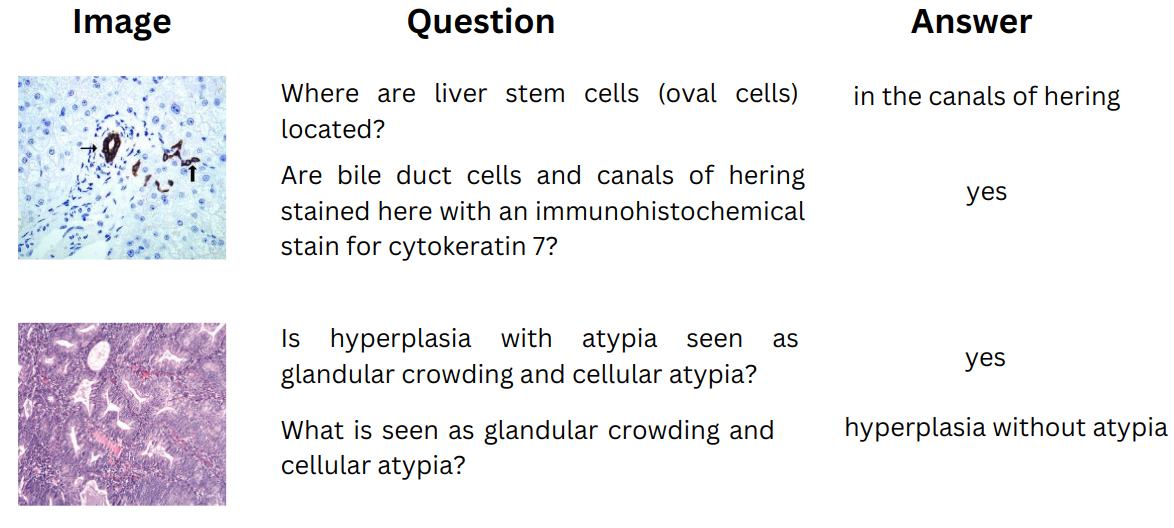
\includegraphics[width=14cm]{image/bab4/sample-pathvqa.png}
  \caption{Sampel data dari \textit{dataset} PathVQA}
  \label{fig:sample-data-pathvqa}
\end{figure}

\begin{figure}[H]
  \centering
  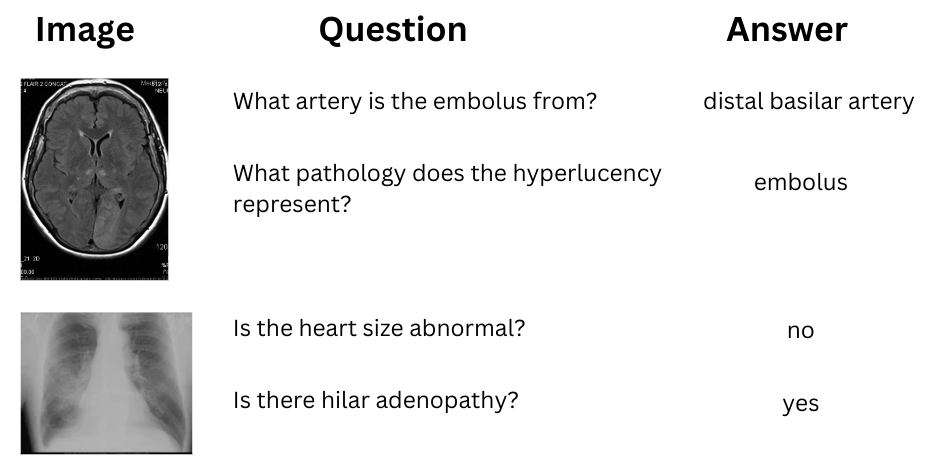
\includegraphics[width=14cm]{image/bab4/sample-vqarad.png}
  \caption{Sampel data dari \textit{dataset} VQA-RAD}
  \label{fig:sample-data-vqarad}
\end{figure}

Kedua \textit{dataset} ini memiliki struktur data bertipe \textit{DatasetDict}, yang merupakan format struktur data khas dari \textit{dataset} Huggingface. Dalam penelitian ini, kedua \textit{dataset} dikonversi menjadi format JSON (\textit{JavaScript Object Notation}) untuk memudahkan penulis dalam mengolah data gambar dan teks. Apabila menggunakan format \textit{DatasetDict}, penulis perlu mengakses data tersebut dengan menerapkan metode atau teknik tertentu sesuai dengan dokumentasi dari Huggingface. Konversi data ke format JSON memungkinkan penulis untuk mengakses dan melakukan pemrosesan data gambar dan teks sesuai dengan keinginan penulis.

\par Pada bagian pemrosesan gambar, penulis menemukan ada beberapa gambar di \textit{dataset} PathVQA yang memiliki format gambar selain \textit{Red Green Blue} (RGB), yaitu \textit{Cyan, Magenta, Yellow, Key (Black)} (CMYK). Pada bagian ini, penulis melakukan konversi gambar CMYK menjadi RGB menggunakan pustaka Python Imaging Library (PIL). Konversi gambar ini dilakukan untuk memastikan bahwa semua gambar dalam \textit{dataset} PathVQA memiliki format gambar yang sama, yaitu RGB. Pada gambar di \textit{dataset} VQA-RAD, semua gambar sudah memiliki format RGB, sehingga tidak perlu dilakukan konversi ke dalam bentuk RGB.

\par Pada bagian pemrosesan teks, kalimat dari pertanyaan telah dilakukan proses \textit{case folding}, \textit{remove punctuation}, \textit{stemming}, dan tokenisasi untuk menghasilkan kalimat yang lebih bersih dan lebih mudah diproses oleh model. 

\par Proses \textit{case folding} dilakukan untuk mengubah seluruh huruf dalam kalimat menjadi huruf kecil, sehingga model dapat memahami kata yang sama dengan huruf besar dan huruf kecil sebagai kata yang sama. Pada Tabel \ref{tab:sample-preprocessing-text-case-folding} terdapat contoh hasil dari proses \textit{case folding}. 

% Please add the following required packages to your document preamble:
% \usepackage{longtable}
% Note: It may be necessary to compile the document several times to get a multi-page table to line up properly
\begin{longtable}[c]{|l|l|}
  \caption{Proses \textit{case folding} pada sampel \textit{dataset} PathVQA dan VQA-RAD}
  \label{tab:sample-preprocessing-text-case-folding}\\
  \hline
  \textbf{Sebelum} &
    \textbf{Sesudah} \\ \hline
  \endfirsthead
  %
  \endhead
  %
  \textit{\begin{tabular}[c]{@{}l@{}}Where are liver stem cells\\  (oval cells) located?\end{tabular}} &
    \textit{\begin{tabular}[c]{@{}l@{}}where are liver stem cells\\  (oval cells) located?\end{tabular}} \\ \hline
  \textit{\begin{tabular}[c]{@{}l@{}}Are bile duct cells and\\  canals of hering stained here \\ with an immunohistochemical\\  stain for cytokeratin 7?\end{tabular}} &
    \textit{\begin{tabular}[c]{@{}l@{}}are bile duct cells and\\  canals of hering stained here \\ with an immunohistochemical\\  stain for cytokeratin 7?\end{tabular}} \\ \hline
  \textit{\begin{tabular}[c]{@{}l@{}}Is hyperplasia with atypia \\ seen as glandular crowding \\ and cellular atypia?\end{tabular}} &
    \textit{\begin{tabular}[c]{@{}l@{}}is hyperplasia with atypia \\ seen as glandular crowding \\ and cellular atypia?\end{tabular}} \\ \hline
  \textit{\begin{tabular}[c]{@{}l@{}}What is seen as glandular\\  crowding and cellular atypia?\end{tabular}} &
    \textit{\begin{tabular}[c]{@{}l@{}}What is seen as glandular\\  crowding and cellular atypia?\end{tabular}} \\ \hline
  \textit{What artery is the embolus from?} &
    \textit{what artery is the embolus from?} \\ \hline
  \textit{\begin{tabular}[c]{@{}l@{}}What pathology does the\\  hyperlucency represent?\end{tabular}} &
    \textit{\begin{tabular}[c]{@{}l@{}}what pathology does the\\  hyperlucency represent?\end{tabular}} \\ \hline
  \textit{Is the heart size abnormal?} &
    \textit{is the heart size abnormal?} \\ \hline
  \textit{Is there hilar adenopathy?} &
    \textit{is there hilar adenopathy?} \\ \hline
  \end{longtable}

\par Setelah proses \textit{case folding}, dilakukan proses \textit{remove punctuation} untuk menghapus tanda baca pada kalimat. Sehingga model dapat memahami kata yang sama dengan tanda baca dan tanpa tanda baca sebagai kata yang sama. Pada Tabel \ref{tab:sample-preprocessing-text-remove-punctuation} terdapat contoh hasil dari proses \textit{remove punctuation}.

% Please add the following required packages to your document preamble:
% \usepackage{longtable}
% Note: It may be necessary to compile the document several times to get a multi-page table to line up properly
\begin{longtable}[c]{|l|l|}
  \caption{Proses \textit{remove punctuation} pada sampel \textit{dataset} PathVQA dan VQA-RAD}
  \label{tab:sample-preprocessing-text-remove-punctuation}\\
  \hline
  \textbf{Sebelum} &
    \textbf{Sesudah} \\ \hline
  \endfirsthead
  %
  \endhead
  %
  \textit{\begin{tabular}[c]{@{}l@{}}where are liver stem cells\\  (oval cells) located?\end{tabular}} &
    \textit{\begin{tabular}[c]{@{}l@{}}where are liver stem cells\\  oval cells located\end{tabular}} \\ \hline
  \textit{\begin{tabular}[c]{@{}l@{}}are bile duct cells and\\ canals of hering stained here \\ with an immunohistochemical\\ stain for cytokeratin 7?\end{tabular}} &
    \textit{\begin{tabular}[c]{@{}l@{}}are bile duct cells and\\ canals of hering stained here \\ with an immunohistochemical\\  stain for cytokeratin 7\end{tabular}} \\ \hline
  \textit{\begin{tabular}[c]{@{}l@{}}is hyperplasia with atypia \\ seen as glandular crowding \\ and cellular atypia?\end{tabular}} &
    \textit{\begin{tabular}[c]{@{}l@{}}is hyperplasia with atypia\\ seen as glandular crowding\\ and cellular atypia\end{tabular}} \\ \hline
  \textit{\begin{tabular}[c]{@{}l@{}}What is seen as glandular\\ crowding and cellular atypia?\end{tabular}} &
    \textit{\begin{tabular}[c]{@{}l@{}}what is seen as glandular\\ crowding and cellular atypia\end{tabular}} \\ \hline
  \textit{what artery is the embolus from?} &
    \textit{what artery is the embolus from} \\ \hline
  \textit{\begin{tabular}[c]{@{}l@{}}what pathology does the\\  hyperlucency represent?\end{tabular}} &
    \textit{\begin{tabular}[c]{@{}l@{}}what pathology does the\\ hyperlucency represent\end{tabular}} \\ \hline
  \textit{is the heart size abnormal?} &
    \textit{is the heart size abnormal} \\ \hline
  \textit{is there hilar adenopathy?} &
    \textit{is there hilar adenopathy} \\ \hline
  \end{longtable}

\par Langkah selanjutnya adalah proses \textit{stemming} yang dilakukan untuk mengubah kata-kata dalam kalimat menjadi kata dasar. Sehingga model dapat memahami kata yang memiliki akar kata yang sama sebagai kata yang sama. Pada Tabel \ref{tab:sample-preprocessing-stemming} terdapat contoh hasil dari proses \textit{stemming}.

% Please add the following required packages to your document preamble:
% \usepackage{longtable}
% Note: It may be necessary to compile the document several times to get a multi-page table to line up properly
\begin{longtable}[c]{|l|l|}
  \caption{Proses \textit{stemming} pada sampel \textit{dataset} PathVQA dan VQA-RAD}
  \label{tab:sample-preprocessing-stemming}\\
  \hline
  \textbf{Sebelum} &
    \textbf{Sesudah} \\ \hline
  \endfirsthead
  %
  \endhead
  %
  \textit{\begin{tabular}[c]{@{}l@{}}where are liver stem cells\\  oval cells located\end{tabular}} &
    \textit{\begin{tabular}[c]{@{}l@{}}where are liver stem cell\\ oval cell locat\end{tabular}} \\ \hline
  \textit{\begin{tabular}[c]{@{}l@{}}are bile duct cells and\\ canals of hering stained here \\ with an immunohistochemical\\ stain for cytokeratin 7\end{tabular}} &
    \textit{\begin{tabular}[c]{@{}l@{}}are bile duct cell and\\ canal of here stain here\\ with an immunohistochem\\ stain for cytokeratin 7\end{tabular}} \\ \hline
  \textit{\begin{tabular}[c]{@{}l@{}}is hyperplasia with atypia\\ seen as glandular crowding\\ and cellular atypia\end{tabular}} &
    \textit{\begin{tabular}[c]{@{}l@{}}is hyperplasia with atypia\\ seen as glandular crowd\\ and cellular atypia\end{tabular}} \\ \hline
  \textit{\begin{tabular}[c]{@{}l@{}}what is seen as glandular\\ crowding and cellular atypia\end{tabular}} &
    \textit{\begin{tabular}[c]{@{}l@{}}what is seen as glandular\\ crowd and cellular atypia\end{tabular}} \\ \hline
  \textit{what artery is the embolus from} &
    \textit{what arteri is the embolu from} \\ \hline
  \textit{\begin{tabular}[c]{@{}l@{}}what pathology does the\\ hyperlucency represent\end{tabular}} &
    \textit{\begin{tabular}[c]{@{}l@{}}what patholog doe the\\ hyperluc repres\end{tabular}} \\ \hline
  \textit{is the heart size abnormal} &
    \textit{is the heart size abnorm} \\ \hline
  \textit{is there hilar adenopathy} &
    \textit{is there hilar adenopathi} \\ \hline
  \end{longtable}

\par Lalu, setelah proses \textit{stemming}, dilakukan proses tokenisasi untuk mengubah kalimat menjadi token. Tokenisasi dilakukan untuk memecah kalimat menjadi kata-kata yang lebih kecil, sehingga model dapat memahami kata-kata dalam kalimat sebagai token. Pada Tabel \ref{tab:sample-preprocessing-tokenization} terdapat contoh hasil dari proses tokenisasi pada sampel \textit{dataset} PathVQA dan VQA-RAD.

% Please add the following required packages to your document preamble:
% \usepackage{longtable}
% Note: It may be necessary to compile the document several times to get a multi-page table to line up properly
\begin{longtable}[c]{|l|l|l}
  \caption{Proses tokenisasi pada sampel dataset PathVQA dan VQA-RAD}
  \label{tab:sample-preprocessing-tokenization}\\
  \cline{1-2}
  \textbf{Sebelum} & \textbf{Sesudah} &  \\ \cline{1-2}
  \endfirsthead
  %
  \endhead
  %
  \textit{where are liver stem cell oval cell locat} & \textit{\begin{tabular}[c]{@{}l@{}}{[}where, are, liver, stem, cell, oval, cell,\\ locat{]}\end{tabular}} &  \\ \cline{1-2}
  \textit{\begin{tabular}[c]{@{}l@{}}are bile duct cell and canal of here stain\\ here with an immunohistochem stain\\ for cytokeratin 7\end{tabular}} & \textit{\begin{tabular}[c]{@{}l@{}}{[}are, bile, duct, cell, and, canal, of, here,\\ stain, here, with, an, immunohistochem, \\ stain, for, cytokeratin, 7{]}\end{tabular}} &  \\ \cline{1-2}
  \textit{\begin{tabular}[c]{@{}l@{}}is hyperplasia with atypia seen as\\ glandular crowd and cellular atypia\end{tabular}} & \textit{\begin{tabular}[c]{@{}l@{}}{[}is, hyperplasia, with, atypia, seen, as, \\ glandular, crowd, and, cellular, atypia{]}\end{tabular}} &  \\ \cline{1-2}
  \textit{\begin{tabular}[c]{@{}l@{}}what is seen as glandular crowd \\ and cellular atypia\end{tabular}} & \textit{\begin{tabular}[c]{@{}l@{}}{[}what, is, seen, as, glandular, crowd, \\ and, cellular, atypia{]}\end{tabular}} &  \\ \cline{1-2}
  \textit{what arteri is the embolu from} & \textit{{[}what, arteri, is, the, embolu, from{]}} &  \\ \cline{1-2}
  \textit{what patholog doe the hyperluc repres} & \textit{\begin{tabular}[c]{@{}l@{}}{[}what, patholog, doe, the, hyperluc,\\ repres{]}\end{tabular}} &  \\ \cline{1-2}
  \textit{is the heart size abnorm} & \textit{{[}is, the, heart, size, abnorm{]}} &  \\ \cline{1-2}
  \textit{is there hilar adenopathi} & \textit{{[}is, there, hilar, adenopathi{]}} &  \\ \cline{1-2}
  \end{longtable}


\par Setelah semua data gambar dan teks telah dilakukan pemrosesan, data tersebut kemudian dibagi menjadi data latih, data validasi, dan data uji. Data latih digunakan untuk melatih model, data validasi digunakan untuk mengevaluasi model selama proses pelatihan, dan data uji digunakan untuk mengevaluasi model setelah proses pelatihan selesai. Rasio pembagian data latih, data validasi, dan data uji pada \textit{dataset} PathVQA dan VQA-RAD adalah 80\%, 10\%, dan 10\%.

\section{Pengembangan Model}

\par Adapun langkah-langkah yang dilakukan dalam pembangunan model VQA dengan arsitektur VGG19-LSTM dan BLIP adalah sebagai berikut:

\subsection{VGG19-LSTM}

\par Pengembangan model dengan VGG19-LSTM dilakukan menggunakan pustaka \textit{TensorFlow} versi 2.11.0. Model VGG19 yang telah dilatih pada \textit{dataset} ImageNet digunakan sebagai \textit{pretrained model} untuk mengekstraksi fitur dari gambar yang telah di \textit{resize} menjadi $224 \times 224$ piksel. Fitur ini kemudian digabungkan dengan fitur teks yang diolah menggunakan GloVe \textit{embedding layer} berdimensi 100. Fitur teks ini mengubah teks menjadi vektor numerik yang dapat diproses oleh model. Fitur gabungan ini kemudian dijadikan sebagai \textit{input} untuk LSTM yang memiliki 128 unit, yang bertugas memprediksi jawaban dari pertanyaan yang diberikan berdasarkan fitur gabungan tersebut.

\par Dalam pemrosesan teks, teks yang telah dilakukan pemrosesan sebelumnya diubah menjadi vektor dengan menggunakan GloVe \textit{embedding}. Setiap kata dalam teks pertanyaan yang terdapat dalam GloVe diwakili sebagai vektor 100 dimensi. Proses ini memungkinkan model untuk menginterpretasikan pertanyaan dalam bentuk numerik yang lebih mudah diproses oleh jaringan saraf. Dalam menangani data jawaban dilakukan suatu teknik bernama \textit{one-hot encoding}. Teknik \textit{one-hot encoding} digunakan untuk merepresentasikan jawaban yang mungkin. Pada hal ini, representasi \textit{one-hot encoding}, setiap jawaban diubah menjadi sebuah vektor di mana hanya satu elemen yang bernilai satu dan sisanya bernilai nol. Panjang vektor ini sesuai dengan jumlah total jawaban yang mungkin. Proses ini mengubah kategori jawaban menjadi format yang dapat langsung diproses oleh lapisan \textit{softmax} dari model, yang memudahkan model dalam melakukan klasifikasi dan menghitung \textit{loss} dengan efektif menggunakan fungsi \textit{loss categorical crossentropy}. Dengan ini, setiap probabilitas \textit{output} dari model langsung mencerminkan kepercayaan model terhadap masing-masing kategori jawaban yang mungkin, memfasilitasi interpretasi yang lebih mudah dan evaluasi performa model yang lebih akurat.

\par \textit{Output} dari lapisan VGG19 dan LSTM kemudian digabungkan melalui operasi \textit{concatenate}. Gabungan fitur ini diolah lebih lanjut menggunakan lapisan \textit{fully connected} dengan 256 unit dan fungsi aktivasi \textit{Rectified Linear Unit} ReLU, dilanjutkan dengan lapisan \textit{output} yang menggunakan fungsi aktivasi \textit{softmax} untuk mengklasifikasikan jawaban dari beberapa pilihan jawaban yang mungkin. Struktur dari model VGG19-LSTM yang digunakan dalam penelitian pada saat melatih \textit{dataset} PathVQA dan VQA-RAD dapat dilihat pada Gambar \ref{fig:struktur-arstektur-vgg19-lstm}.

\begin{figure}[H]
  \centering
  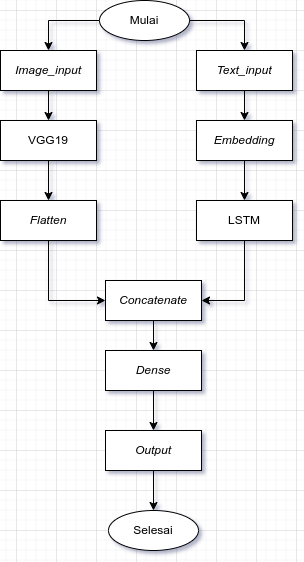
\includegraphics[width = 7cm, height= 14cm]{image/bab4/vgg19-lstm-struktur.png}
  \caption{Struktur arsitektur VGG19-LSTM}
  \label{fig:struktur-arstektur-vgg19-lstm}
\end{figure}

\par Berdasarkan Gambar \ref{fig:struktur-arstektur-vgg19-lstm}, model VGG19-LSTM terdiri dari beberapa lapisan, penjelasan dari setiap lapisan tersebut adalah sebagai berikut:

\begin{enumerate}
  \item Lapisan "\textit{image\_input}" adalah lapisan \textit{input} untuk gambar yang menerima gambar dengan ukuran $224 \times 224$ piksel dan 3 saluran warna (RGB). Lapisan ini tidak memiliki parameter yang bisa dilatih karena hanya berfungsi sebagai \textit{input}.

  \item Lapisan "\textit{text\_input}" adalah lapisan \textit{input} untuk teks yang menerima teks dengan panjang maksimal 24 kata (atau token). Seperti halnya "\textit{image\_input}", lapisan ini juga tidak memiliki parameter yang bisa dilatih karena hanya berfungsi sebagai \textit{input}.

  \item Lapisan "vgg19" adalah model VGG19 yang sudah dilatih sebelumnya, digunakan untuk ekstraksi fitur gambar. \textit{Output} dari lapisan ini adalah tensor dengan dimensi yang belum ditentukan (akan ditentukan saat runtime) dan memiliki 512 fitur. Lapisan ini terhubung ke lapisan "\textit{image\_input}" karena menerima \textit{output} dari lapisan tersebut.

  \item Lapisan "\textit{embedding}" adalah lapisan yang mengubah token teks menjadi vektor \textit{embedding}. \textit{Output} dari lapisan ini adalah tensor dengan panjang 24 dan vektor \textit{embedding} dengan 100 dimensi. Lapisan ini terhubung ke lapisan "\textit{text\_input}" karena menerima \textit{output} dari lapisan tersebut.

  \item Lapisan "\textit{flatten}" adalah lapisan yang mengubah tensor multi-dimensi menjadi vektor 1 dimensi. \textit{Output} dari lapisan ini adalah vektor dengan panjang 25.088. Lapisan ini terhubung ke \textit{output} dari lapisan "vgg19" karena menerima \textit{output} dari lapisan tersebut.

  \item Lapisan "lstm" adalah lapisan LSTM yang mengolah urutan \textit{embedding} teks. \textit{Output} dari lapisan ini adalah tensor dengan 128 unit. Lapisan ini terhubung ke \textit{output} dari lapisan "\textit{embedding}" karena menerima \textit{output} dari lapisan tersebut.

  \item Lapisan "\textit{concatenate}" adalah lapisan yang menggabungkan fitur gambar dan teks. \textit{Output} dari lapisan ini adalah tensor gabungan dengan panjang 25.216. Lapisan ini terhubung ke \textit{output} dari lapisan "flatten" dan "lstm" karena menerima \textit{output} dari kedua lapisan tersebut.

  \item Lapisan "\textit{dense}" setelah lapisan "\textit{concatenate}" adalah lapisan "\textit{dense}" dengan 256 unit. \textit{Output} dari lapisan ini adalah tensor dengan 256 unit. Lapisan ini terhubung ke \textit{output} dari lapisan "\textit{concatenate}" karena menerima \textit{output} dari lapisan tersebut.

  \item Lapisan "\textit{output}" adalah lapisan yang digunakan untuk prediksi akhir dengan 4879 kelas pada \textit{dataset} PathVQA dan 517 kelas pada \textit{dataset} VQA-RAD. \textit{Output} dari lapisan ini adalah tensor dengan 4879 unit (kelas) pada \textit{dataset} PathVQA dan 517 unit (kelas) pada \textit{dataset} VQA-RAD.

\end{enumerate}


\par Struktur dari model VGG19-LSTM yang dilatih dengan \textit{dataset} PathVQA dan VQA-RAD hanya berbeda pada lapisan terakhir, yaitu lapisan "dense" yang memiliki jumlah kelas yang berbeda. Pada \textit{dataset} PathVQA, jumlah kelas yang digunakan adalah 4879 kelas, sedangkan pada \textit{dataset} VQA-RAD, jumlah kelas yang digunakan adalah 517 kelas. Hal ini disebabkan oleh perbedaan jumlah kelas jawaban pada kedua \textit{dataset}. Sehingga, model VGG19-LSTM yang dilatih dengan \textit{dataset} PathVQA memiliki parameter yang lebih banyak dibandingkan dengan model VGG19-LSTM yang dilatih dengan \textit{dataset} VQA-RAD. Jumlah parameter pada model VGG19-LSTM yang dilatih dengan \textit{dataset} PathVQA adalah 27.851.187, sedangkan jumlah parameter pada model VGG19-LSTM yang dilatih dengan \textit{dataset} VQA-RAD adalah 26.730.153.

\par Model ini dikompilasi dengan menggunakan fungsi optimasi Adam dan menggunakan fungsi \textit{loss categorical crossentropy} dikarenakan masalah yang dihadapi adalah masalah klasifikasi multikelas. Dengan adanya fungsi optimasi disini navigasi ruang parameter dapat terjadi yaitu dengan adanya fungsi optimasi yang bekerja dengan menghitung gradien dari fungsi \textit{loss} terhadap masing-masing parameter model. Gradien disini dapat memberitahu fungsi optimasi arah untuk mengubah parameter guna mengurangi \textit{loss}. Secara intuitif, gradien akan menunjukkan arah tercepat untuk turun dari bukit dalam ruang parameter menuju ke titik terendah. Sehingga, model dapat belajar dari data latih dan meningkatkan performa model secara iteratif.

\par Secara keseluruhan, model VGG19-LSTM yang dilatih dengan \textit{dataset} PathVQA dan VQA-RAD memiliki arsitektur yang sama, namun berbeda pada jumlah kelas yang digunakan. Model ini memiliki tiga lapisan utama, yaitu lapisan VGG19, lapisan LSTM, dan lapisan \textit{output} yang digunakan untuk memprediksi jawaban. Model ini memiliki kemampuan untuk memproses gambar dan teks secara bersamaan, dan menghasilkan prediksi jawaban berdasarkan gambar dan pertanyaan yang diberikan.

\subsection{BLIP}

\par Pengembangan model dengan BLIP dilakukan menggunakan pustaka PyTorch versi 2.0.1 dan Transformers versi 4.31.0. Di sini, PyTorch digunakan sebagai \textit{deep learning framework} untuk melatih model, sedangkan Transformers digunakan untuk mengakses \textit{pre-trained} model BLIP. Sebelum melatih model dengan BLIP, penulis melakukan pemrosesan khusus pada data gambar dan data teks menggunakan pustaka Transformers dari Huggingface untuk mengkonversi data tersebut menjadi format yang dapat diproses oleh BLIP. Pustaka Transformers yang digunakan adalah \textit{BlipImageProcessor} dan \textit{BlipProcessor}. Kedua pustaka ini mengkonversi data gambar dan teks menjadi format yang sesuai untuk pemrosesan oleh BLIP.

% \par Dalam arsitektur BLIP, beberapa bagian dari encoder menggunakan GELU (\textit{Gaussian Error Linear Unit}) sebagai fungsi aktivasi. Fungsi aktivasi ini diterapkan antara lapisan-lapisan linear, yang memfasilitasi transformasi input dari satu dimensi ke dimensi lain sebelum memasuki lapisan output. GELU memberikan kontribusi penting dalam meningkatkan performa model berbasis transformer seperti BLIP, karena memungkinkan pemrosesan informasi yang lebih halus dan adaptif. Hal ini membantu model untuk memahami dan mengintegrasikan data dengan lebih efektif, sehingga meningkatkan akurasi dan efisiensi dalam menghasilkan respons yang tepat berdasarkan pertanyaan visual yang diajukan. 

\par Pada model BLIP, data gambar diolah menggunakan \textit{BlipImageProcessor} dari pustaka Transformers. Fungsi \textit{BlipImageProcessor} mengubah ukuran gambar menjadi $128 \times 128$ piksel, dan mengubah gambar yang telah diolah menjadi format tensor yang dapat diproses oleh model BLIP. Sedangkan, untuk data teks diolah menggunakan \textit{BlipProcessor}. Dalam hal ini, \textit{BlipProcessor} melakukan tugas-tugas khusus seperti \textit{padding}, \textit{truncation}, dan \textit{encoding}. \textit{Padding} bertugas menambahkan token khusus pada data teks untuk memastikan bahwa semua data teks memiliki panjang yang sama. \textit{Truncation} bertugas memotong data teks yang melebihi panjang maksimum yang telah ditentukan, yaitu 32 token. \textit{Encoding} mengkonversi data teks menjadi format numerik yang dapat diproses oleh model BLIP.

\par Setelah data gambar dan teks diolah, penulis kemudian mengunduh model yang telah dilatih sebelumnya dari BLIP, yang digunakan untuk tugas \textit{Visual Question Answering} (VQA) menggunakan pustaka Transformers. Model ini dilatih pada \textit{dataset} Visual Genome dan VQA v2.0, dan kemudian dilakukan \textit{fine-tuning} menggunakan \textit{dataset} PathVQA dan VQA-RAD. Dalam proses \textit{fine-tuning} ini, model BLIP dilatih menggunakan fungsi optimasi Adam dan fungsi \textit{loss} \textit{categorical crossentropy}, karena masalah yang dihadapi adalah klasifikasi multikelas. Fungsi optimasi Adam di sini memainkan peran penting dalam meminimalkan nilai \textit{loss} yang dihasilkan oleh fungsi \textit{loss} \textit{categorical crossentropy}. Fungsi \textit{loss} mengukur kesalahan prediksi model terhadap kelas yang sebenarnya, dan nilai \textit{loss} yang lebih rendah menunjukkan kesesuaian yang lebih baik antara prediksi model dan kenyataan. Fungsi optimasi, dalam hal ini Adam, secara efektif mengatur proses pembaharuan bobot model berdasarkan gradien dari fungsi \textit{loss}. Proses ini penting untuk mengarahkan model agar mencapai efisiensi maksimal dalam memprediksi kelas yang benar, secara bertahap menurunkan kesalahan prediksi sepanjang iterasi pelatihan. Oleh karena itu, pemilihan fungsi optimasi yang tepat sangat krusial untuk memastikan keberhasilan \textit{fine-tuning} model dalam mencapai hasil yang akurat dan relevan. 

\par Struktur model BLIP pada tugas \textit{Visual Question Answering (VQA)} terdiri dari tiga lapisan utama, yaitu \textit{vision\_model}, \textit{text\_encoder}, dan \textit{text\_decoder}. Ketiga lapisan ini berfungsi untuk memproses \textit{input} gambar dan teks, serta menghasilkan prediksi jawaban akhir berdasarkan gambar dan pertanyaan yang diberikan. Struktur dari ketiga lapisan ini dapat dilihat pada Lampiran 1, Lampiran 2, dan Lampiran 3.


\par Lapisan \textit{vision\_model} bertugas untuk memproses \textit{input} gambar dan terdiri dari dua bagian utama: \textit{embeddings} dan \textit{encoder}. Di bagian \textit{embeddings} menggunakan \textit{backbone Vision Transformer} (ViT) untuk mengubah gambar menjadi \textit{patch embedding}. Bagian \textit{encoder} terdiri dari beberapa lapisan \textit{encoder} yang menangkap hubungan antar \textit{patch} gambar menggunakan mekanisme \textit{self-attention}. Setiap \textit{layer encoder} dilengkapi dengan normalisasi dan \textit{Multi-Layer Perceptron} (MLP) dengan aktivasi \textit{Gaussian Error Linear Unit} (GELU) untuk transformasi lebih lanjut. Berikut adalah penjelasan dari setiap lapisan dalam \textit{vision\_model}:

\begin{enumerate}

    \item \textit{Embeddings}: Ini merupakan komponen dari \textit{BlipVisionModel} yang menggunakan \textit{BlipVisionEmbeddings} untuk menerapkan konvolusi 2D (Conv2d) dengan menggunakan \textit{backbone} ViT untuk mengubah gambar menjadi representasi vektor dari potongan-potongan gambar (\textit{patches}).

    \item \textit{BlipVisionEmbeddings}: Ini merupakan komponen yang mencakup \textit{patch embeddings} menggunakan Conv2d. Dimensi \textit{input} adalah 3 saluran warna RGB, dimensi \textit{output} adalah 768, ukuran kernel $16 \times 16$, dan stride $16 \times 16$.

    \item \textit{Encoder}: Bagian yang mencakup \textit{BlipEncoder} yang terdiri dari beberapa lapisan \textit{encoder} yang masing-masing menggunakan mekanisme \textit{self-attention} untuk menangkap hubungan antar \textit{patch} gambar.

    \item \textit{BlipEncoder}: Ini merupakan komponen utama \textit{encoder} yang terdiri dari beberapa \textit{BlipEncoderLayer}, dengan jumlah total 12 lapisan.

    \item \textit{BlipEncoderLayer}: Bagian dari \textit{BlipEncoder} yang dimana setiap lapisan yang terdiri dari bagian terdapat beberapa subkomponen yaitu \textit{self-attention}, MLP, dua \textit{LayerNorm}. Di bagian ini, \textit{input} dari gambar diolah menggunakan mekanisme \textit{self-attention} dan MLP untuk transformasi lebih lanjut.

    \item \textit{BlipAttention}: Bagian ini menangkap hubungan antar \textit{patch} gambar menggunakan mekanisme \textit{self-attention}. Komponen ini menggunakan \textit{query}, \textit{key}, dan \textit{value} dengan dimensi $768 \times 2304$ dan proyeksi dengan dimensi $768 \times 768$. Nilai \textit{dropout} adalah 0,0.

    \item \textit{BlipMLP}: Menggunakan lapisan linear untuk transformasi lebih lanjut dari hasil \textit{attention} dan fungsi aktivasi GELU untuk menambah non-linearitas. Lapisan pertama (fc1) memiliki dimensi $768 \times 3072$ dan lapisan kedua (fc2) memiliki dimensi $3072 \times 768$.

    \item \textit{LayerNorm}: Digunakan untuk normalisasi pada beberapa bagian model, termasuk \textit{layer\_norm1}, \textit{layer\_norm2}, dan \textit{post\_layernorm}. Parameter \textit{LayerNorm} memiliki nilai epsilon $1 \times 10^{-5}$.

    \item \textit{PostLayerNorm}: Merupakan lapisan normalisasi akhir setelah seluruh lapisan \textit{encoder} selesai memproses \textit{input}. Tujuannya adalah untuk menstabilkan dan menormalisasi keluaran akhir dari \textit{encoder} sebelum digunakan oleh bagian lain dari model.


  
\end{enumerate}

\par Lapisan \textit{text\_encoder} bertugas untuk memproses \textit{input} teks dan terdiri dari dua bagian utama: \textit{embeddings} dan \textit{encoder}. Bagian \textit{embeddings} menyediakan representasi kata dan posisi dalam teks, sementara bagian \textit{encoder} terdiri dari beberapa lapisan yang menangkap hubungan antar kata menggunakan mekanisme \textit{attention}. Selain \textit{self-attention}, terdapat \textit{cross-attention} yang menangkap hubungan antara teks dan fitur gambar jika ada. Setiap \textit{layer encoder} juga dilengkapi dengan normalisasi dan MLP untuk transformasi lebih lanjut. Berikut adalah penjelasan dari setiap lapisan dalam \textit{text\_encoder}:

\begin{enumerate}

  \item \textit{Embeddings}: Pada bagian ini terdiri dari \textit{word embeddings} yang merupakan representasi vektor dari kata-kata dalam teks dan \textit{position embeddings} yang memberikan informasi posisi dari setiap kata dalam teks. Jumlah fitur yang digunakan adalah 768 dengan \textit{padding} indeks 0.

  \item \textit{BlipTextEmbeddings}: Ini merupakan komponen yang mencakup \textit{word embeddings} dan \textit{position embeddings}, serta menggunakan \textit{LayerNorm} untuk normalisasi dan \textit{dropout} untuk mengurangi \textit{overfitting}. Dimensi \textit{word embeddings} adalah $30524 \times 768$ dimensi, sedangkan dimensi \textit{position embeddings} adalah $512 \times 768$ dimensi. Parameter \textit{LayerNorm} memiliki nilai epsilon $1 \times 10^{-12}$, dengan nilai \textit{dropout} 0,0.

  \item \textit{Encoder}: Pada bagian ini terdiri dari beberapa lapisan yang masing-masing menggunakan mekanisme \textit{attention} untuk menangkap hubungan antar kata. Hal ini bertujuan untuk memahami dan mengintegrasikan informasi pada pertanyaan yang diajukan.

  \item \textit{BlipTextEncoder}: Ini merupakan komponen \textit{encoder} yang terdiri dari beberapa lapisan \textit{BlipTextLayer}. 

  \item \textit{BlipTextLayer}: Setiap lapisan terdiri dari beberapa subkomponen yaitu \textit{attention}, \textit{crossattention}, \textit{intermediate}, dan \textit{output}, dengan jumlah total 12 lapisan \textit{BlipTextLayer}.

  \item \textit{BlipTextAttention}: Hal ini berguna untuk menangkap hubungan antar kata dalam teks menggunakan \textit{self-attention} dan hubungan antara teks dan fitur gambar menggunakan \textit{cross-attention}. Dimensi \textit{query}, \textit{key}, dan \textit{value} masing-masing adalah $768 \times 768$ dengan nilai \textit{dropout} 0,0.

  \item \textit{BlipTextSelfAttention}: Bagian dari \textit{BlipTextAttention} yang menggunakan \textit{query}, \textit{key}, dan \textit{value} untuk menghitung perhatian antar kata dalam teks, dengan dimensi \textit{query}, \textit{key}, dan \textit{value} masing-masing $768 \times 768$.

  \item \textit{BlipTextSelfOutput}: Bagian ini menghasilkan \textit{output} dari mekanisme \textit{attention} dan menggunakan \textit{LayerNorm} serta \textit{dropout} untuk normalisasi dan mengurangi \textit{overfitting}. Dimensi dense layer adalah $768 \times 768$ dengan parameter \textit{LayerNorm} epsilon $1 \times 10^{-12}$ dan nilai \textit{dropout} 0,0.

  \item \textit{BlipTextIntermediate}: Bagian ini menggunakan lapisan linear untuk transformasi lebih lanjut dari hasil \textit{attention} dan fungsi aktivasi GELU untuk menambah non-linearitas. Dimensi dense layer adalah $768 \times 3072$ dengan fungsi aktivasi GELU.

  \item \textit{BlipTextOutput}: Di sini dihasilkan \textit{output} akhir dari lapisan \textit{encoder} dengan lapisan linear dan \textit{LayerNorm} untuk normalisasi. Dimensi dense layer adalah $3072 \times 768$ dengan parameter \textit{LayerNorm} epsilon $1 \times 10^{-12}$ serta nilai \textit{dropout} 0,0.


\end{enumerate}



\par Lapisan \textit{text\_decoder} bertugas untuk mendekode dan menghasilkan teks dari fitur yang telah diproses, menggunakan struktur yang mirip dengan model \textit{Bidirectional Encoder Representation From Transformers} (BERT). Bagian \textit{decoder} terdiri dari \textit{embeddings} untuk kata dan posisi, serta beberapa lapisan \textit{encoder} yang menggunakan mekanisme \textit{self-attention} dan \textit{cross-attention}. Setiap lapisan dilengkapi dengan MLP dan normalisasi untuk transformasi lebih lanjut. Bagian \textit{cls} dari \textit{decoder} bertugas untuk menghasilkan prediksi jawaban akhir berdasarkan fitur yang telah diproses. Berikut adalah penjelasan dari setiap lapisan dalam \textit{text\_decoder}:

\begin{enumerate}

  \item \textit{Embeddings}: Menggunakan \textit{word embeddings} dan \textit{position embeddings} untuk menyediakan representasi vektor dari kata dan posisi dalam teks. Pada bagian ini, dimensi pada \textit{word embeddings} adalah $30524 \times 768$, sedangkan dimensi \textit{position embeddings} adalah $512 \times 768$. Lapisan ini juga menggunakan \textit{LayerNorm} dengan nilai epsilon $1 \times 10^{-12}$ dan \textit{dropout} dengan nilai 0,0.

  \item \textit{BlipTextEmbeddings}: Bagian ini, merupakan komponen utama yang mencakup \textit{word embeddings} dan \textit{position embeddings}, serta menggunakan \textit{LayerNorm} dan \textit{dropout} untuk normalisasi dan mengurangi \textit{overfitting}. Pada bagian ini, dimensi \textit{word embeddings} adalah $30524 \times 768$, dimensi \textit{position embeddings} adalah $512 \times 768$, nilai epsilon $1 \times 10^{-12}$, dan nilai \textit{dropout} 0,0.

  \item \textit{Encoder}: Terdiri dari beberapa lapisan \textit{encoder} yang menggunakan mekanisme \textit{self-attention} dan \textit{cross-attention} untuk menangkap hubungan antar kata dan antara kata dengan fitur lain. Terdapat total 12 lapisan \textit{BlipTextLayer}.

  \item \textit{BlipTextEncoder}: Ini merupakan komponen utama \textit{encoder} yang terdiri dari beberapa \textit{BlipTextLayer}, dengan jumlah total 12 lapisan.

  \item \textit{BlipTextLayer}: Setiap lapisan terdiri dari beberapa subkomponen yaitu \textit{attention}, \textit{crossattention}, \textit{intermediate}, dan \textit{output}. Lapisan \textit{attention} dan \textit{crossattention} masing-masing menggunakan \textit{self-attention} dengan \textit{query}, \textit{key}, dan \textit{value}, serta proyeksi dengan dimensi $768 \times 768$ dan nilai \textit{dropout} 0,0. Lapisan \textit{intermediate} menggunakan lapisan linear dengan dimensi $768 \times 3072$ dan fungsi aktivasi GELU, sementara lapisan \textit{output} menggunakan lapisan linear dengan dimensi $3072 \times 768$ dan \textit{LayerNorm} dengan nilai epsilon $1 \times 10^{-12}$.

  \item \textit{BlipTextAttention}: Hal ini berguna untuk menangkap hubungan antar kata dalam teks menggunakan mekanisme \textit{self-attention}. Komponen ini menggunakan \textit{query}, \textit{key}, dan \textit{value} dengan dimensi $768 \times 768$ dan proyeksi dengan dimensi $768 \times 768$. Nilai \textit{dropout} adalah 0,0.

  \item \textit{BlipTextSelfAttention}: Bagian dari \textit{BlipTextAttention} yang menggunakan \textit{query}, \textit{key}, dan \textit{value} untuk menghitung perhatian antar kata dalam teks, dengan dimensi \textit{query}, \textit{key}, dan \textit{value} masing-masing $768 \times 768$.

  \item \textit{BlipTextSelfOutput}: Bagian ini, menghasilkan \textit{output} dari mekanisme \textit{attention} dan menggunakan \textit{LayerNorm} serta \textit{dropout} untuk normalisasi dan mengurangi \textit{overfitting}. Dimensi dense layer adalah $768 \times 768$ dengan parameter \textit{LayerNorm} epsilon $1 \times 10^{-12}$ serta nilai \textit{dropout} 0,0.

  \item \textit{BlipTextIntermediate}: Menggunakan lapisan linear untuk transformasi lebih lanjut dari hasil \textit{attention} dan fungsi aktivasi GELU untuk menambah non-linearitas. Dimensi dense layer adalah $768 \times 3072$ dengan fungsi aktivasi GELU.

  \item \textit{BlipTextOutput}: Menghasilkan \textit{output} akhir dari lapisan \textit{encoder} dengan lapisan linear dan \textit{LayerNorm} untuk normalisasi. Dimensi dense layer adalah $3072 \times 768$ dengan parameter \textit{LayerNorm} epsilon $1 \times 10^{-12}$ serta nilai \textit{dropout} 0,0.

  \item \textit{BlipTextOnlyMLMHead}: Bertugas untuk menghasilkan prediksi jawaban akhir berdasarkan fitur yang telah diproses. Bagian dari komponen ini mencakup \textit{BlipTextLMPredictionHead} yang terdiri dari transformasi dan \textit{decoder}. Transform menggunakan lapisan linear dengan dimensi $768 \times 768$, fungsi aktivasi GELU, dan \textit{LayerNorm} dengan nilai epsilon $1 \times 10^{-12}$. Bagian \textit{decoder} menggunakan lapisan linear dengan dimensi $768 \times 30524$.

  \item \textit{BlipTextLMPredictionHead}: Ini merupakan komponen dari \textit{cls} yang mencakup transformasi dan \textit{decoder}. Disini, dilakukan transformasi dengan menggunakan lapisan linear dengan dimensi $768 \times 768$, fungsi aktivasi GELU, dan \textit{LayerNorm} dengan nilai epsilon $1 \times 10^{-12}$. Disini, \textit{decoder} menggunakan lapisan linear dengan dimensi $768 \times 30524$.

  \item \textit{BlipTextPredictionHeadTransform}: Bagian dari \textit{BlipTextLMPredictionHead} yang menggunakan lapisan linear untuk transformasi fitur dengan dimensi $768 \times 768$, fungsi aktivasi GELU, dan \textit{LayerNorm} dengan nilai epsilon $1 \times 10^{-12}$.

\end{enumerate}

Secara keseluruhan, model BLIP pada tugas VQA yang terdiri dari tiga lapisan utama, yaitu \textit{vision\_model}, \textit{text\_encoder}, dan \textit{text\_decoder}, berguna untuk memproses kedua \textit{input} yaitu gambar dan pertanyaan, serta menghasilkan prediksi jawaban akhir berdasarkan kedua \textit{input} tersebut. Dengan adanya tiga lapisan ini, model BLIP dapat memahami dan merespon pertanyaan visual dengan lebih efektif dan efisien, sehingga meningkatkan akurasi dan relevansi jawaban yang dihasilkan, sehingga dapat membantu dalam mendukung pertanyaan dengan konteks visual yang ada.

\section{Augmentasi Data}

\par Pada penelitian ini, dilakukan augmentasi data untuk kalimat pertanyaan pada \textit{dataset} PathVQA dan VQA-RAD. Augmentasi ini menggunakan teknik augmentasi teks dari pustaka nlpaug versi 1.1.11. Teknik ini memanfaatkan fungsi dari nlpaug untuk menghasilkan variasi parafrase dari setiap pertanyaan dalam \textit{dataset}. Pada penelitian ini, setiap pertanyaan diubah menjadi tujuh variasi yang berbeda. Setiap versi parafrase dari pertanyaan tersebut kemudian dibuat sebagai entri baru dalam \textit{dataset}, di mana setiap entri baru masih mengacu pada gambar dan jawaban yang sama dengan pertanyaan asli. Metode augmentasi ini meningkatkan variasi linguistik dalam \textit{dataset}, yang sangat bermanfaat untuk melatih model NLP agar dapat memahami dan merespon berbagai formulasi pertanyaan secara lebih efektif. Augmentasi dilakukan dengan menggunakan sinonim dari leksikal WordNet untuk menghasilkan sinonim untuk kata-kata dalam kalimat yang ada, sehingga menghasilkan variasi parafrase dari kalimat asli. Pada saat proses augmentasi ada bermunculan data yang duplikat, oleh karena itu penulis melakukan penghapusan data duplikat tersebut. Dengan menerapkan teknik augmentasi ini, awalnya \textit{dataset} PathVQA memiliki 32.632 data, setelah dilakukan augmentasi data menjadi 179.167 data. Sedangkan \textit{dataset} VQA-RAD yang awalnya memiliki 2.248 data, setelah dilakukan augmentasi data menjadi 14.347 data. Pada hal ini tujuan dilakukan augmentasi data karena pertanyaan terkait masalah medis sangatlah beragam dan kompleks, sehingga diperlukan variasi pertanyaan yang lebih banyak dan mengatasi kurangnya variasi pertanyaan pada \textit{dataset} yang ada. Pada Tabel \ref{tab:augmentasi-data} menunjukkan contoh pertanyaan yang telah diaugmentasi dengan memanfaatkan teknik augmentasi teks dari pustaka nlpaug dengan menggunakan sinonim dari leksikal WordNet.

% Please add the following required packages to your document preamble:
% \usepackage{multirow}
% \usepackage{graphicx}
\begin{table}[H]
  \centering
  \caption{Contoh pertanyaan yang telah diaugmentasi}
  \label{tab:augmentasi-data}
  \resizebox{\textwidth}{!}{%
  \begin{tabular}{|l|l|}
  \hline
  \textbf{Pertanyaan original} & \textbf{Pertanyaan augmentasi}                                                                                                        \\ \hline
  \multirow{7}{*}{\textit{\begin{tabular}[c]{@{}l@{}}What is the primary use of MRI \\ in medical diagnosis?\end{tabular}}} &
    \textit{\begin{tabular}[c]{@{}l@{}}What is the elemental use of magnetic resonance\\ imaging in aesculapian diagnosis?\end{tabular}} \\ \cline{2-2} 
                               & \textit{\begin{tabular}[c]{@{}l@{}}What be the primary usance of magnetic resonance\\ imaging in medical diagnosis?\end{tabular}}     \\ \cline{2-2} 
                               & \textit{\begin{tabular}[c]{@{}l@{}}What embody the main use of magnetic resonance\\ imaging in aesculapian diagnosis?\end{tabular}}   \\ \cline{2-2} 
                               & \textit{\begin{tabular}[c]{@{}l@{}}What is the primary habit of magnetic resonance \\ imaging in medical diagnosis?\end{tabular}}     \\ \cline{2-2} 
                               & \textit{What be the primary use of MRI in medical diagnosis?}                                                                         \\ \cline{2-2} 
                               & \textit{\begin{tabular}[c]{@{}l@{}}What is the primary usance of magnetic resonance\\ imaging in aesculapian diagnosis?\end{tabular}} \\ \cline{2-2} 
                               & \textit{\begin{tabular}[c]{@{}l@{}}What be the primary use of magnetic resonance\\ imaging in medical diagnosis?\end{tabular}}        \\ \hline
  \end{tabular}%
  }
  \end{table}


\section{Analisis Hasil}

\par Dalam rangka melakukan eksperimen, penulis telah melakukan konfigurasi dari berbagai \textit{hyperparameter} untuk melatih model VGG19-LSTM dan BLIP, dengan tujuan meningkatkan efektivitas dan efisiensi pelatihan. Dalam hal ini, \textit{hyperparameter} yang diatur mencakup jumlah \textit{epochs}, \textit{learning rate}, dan \textit{batch size}. Peran ketiga \textit{hyperparameter} ini memiliki peran penting dalam menentukan keberhasilan pelatihan model, karena mempengaruhi proses optimisasi model untuk mencapai hasil yang optimal. \textit{Hyperparameter} ini memungkinkan penyesuaian yang lebih spesifik terhadap karakteristik data dan kebutuhan eksperimental, sehingga memungkinkan model untuk belajar dengan lebih baik dan menghasilkan respons yang lebih akurat terhadap pertanyaan visual yang diajukan. Tabel \ref{tab:konfigurasi-hyperparameter-model} menunjukkan konfigurasi \textit{hyperparameter} yang digunakan dalam eksperimen ini untuk melatih model VGG19-LSTM dan BLIP dengan \textit{dataset} PathVQA dan VQA-RAD, sebelum dilakukan augmentasi data. Hal ini dilakukan untuk melihat pengaruh konfigurasi \textit{hyperparameter} terhadap performa model pada data asli sebelum dilakukan augmentasi.
  
% Please add the following required packages to your document preamble:
% \usepackage{multirow}
\begin{table}[H]
  \centering
  \caption{Konfigurasi \textit{hyperparameter} pada awal eksperimen}  
  \label{tab:konfigurasi-hyperparameter-model}
  \begin{tabular}{|c|ccc|}
  \hline
  \multirow{2}{*}{\textbf{No}} & \multicolumn{3}{c|}{\textbf{Konfigurasi \textit{hyperparameter}}} \\ \cline{2-4} 
   & \multicolumn{1}{c|}{\textbf{\textit{Epochs}}} & \multicolumn{1}{c|}{\textbf{\textit{Learning rate}}} & \textbf{\textit{Batch size}} \\ \hline
  \multirow{6}{*}{1} & \multicolumn{1}{c|}{\multirow{6}{*}{15}} & \multicolumn{1}{c|}{\multirow{3}{*}{$1 \times 10^{-5}$}} & 8 \\ \cline{4-4} 
   & \multicolumn{1}{c|}{} & \multicolumn{1}{c|}{} & 16 \\ \cline{4-4} 
   & \multicolumn{1}{c|}{} & \multicolumn{1}{c|}{} & 32 \\ \cline{3-4} 
   & \multicolumn{1}{c|}{} & \multicolumn{1}{c|}{\multirow{3}{*}{$5 \times 10^{-5}$}} & 8 \\ \cline{4-4} 
   & \multicolumn{1}{c|}{} & \multicolumn{1}{c|}{} & 16 \\ \cline{4-4} 
   & \multicolumn{1}{c|}{} & \multicolumn{1}{c|}{} & 32 \\ \hline
  \multirow{6}{*}{2} & \multicolumn{1}{c|}{\multirow{6}{*}{30}} & \multicolumn{1}{c|}{\multirow{3}{*}{$1 \times 10^{-5}$}} & 8 \\ \cline{4-4} 
   & \multicolumn{1}{c|}{} & \multicolumn{1}{c|}{} & 16 \\ \cline{4-4} 
   & \multicolumn{1}{c|}{} & \multicolumn{1}{c|}{} & 32 \\ \cline{3-4} 
   & \multicolumn{1}{c|}{} & \multicolumn{1}{c|}{\multirow{3}{*}{$5 \times 10^{-5}$}} & 8 \\ \cline{4-4} 
   & \multicolumn{1}{c|}{} & \multicolumn{1}{c|}{} & 16 \\ \cline{4-4} 
   & \multicolumn{1}{c|}{} & \multicolumn{1}{c|}{} & 32 \\ \hline
  \multirow{6}{*}{3} & \multicolumn{1}{c|}{\multirow{6}{*}{45}} & \multicolumn{1}{c|}{\multirow{3}{*}{$1 \times 10^{-5}$}} & 8 \\ \cline{4-4} 
   & \multicolumn{1}{c|}{} & \multicolumn{1}{c|}{} & 16 \\ \cline{4-4} 
   & \multicolumn{1}{c|}{} & \multicolumn{1}{c|}{} & 32 \\ \cline{3-4} 
   & \multicolumn{1}{c|}{} & \multicolumn{1}{c|}{\multirow{3}{*}{$5 \times 10^{-5}$}} & 8 \\ \cline{4-4} 
   & \multicolumn{1}{c|}{} & \multicolumn{1}{c|}{} & 16 \\ \cline{4-4} 
   & \multicolumn{1}{c|}{} & \multicolumn{1}{c|}{} & 32 \\ \hline
  \end{tabular}
  \end{table}


\par Konfigurasi \textit{hyperparameter} yang digunakan dalam eksperimen ini merupakan pilihan berdasarkan preferensi peneliti untuk mendapatkan kombinasi awal yang rasional. Eksperimen dengan jumlah \textit{epochs} 15, 30, dan 45, \textit{batch size} 8, 16, dan 32, serta \textit{learning rate} sebesar $1 \times 10^{-5}$, dan $5 \times 10^{-5}$. Dengan menggunakan kombinasi \textit{hyperparameter} ini, penulis akan mencari kombinasi yang paling optimal dengan menggunakan metode \textit{grid search} untuk mencari kombinasi \textit{hyperparameter} yang paling optimal.


\par Dari hasil eksperimen yang dilakukan dengan VGG19-LSTM dengan \textit{dataset} PathVQA dan VQA-RAD didapatlah hasil untuk pengujian pada pertanyaan yang bersifat \textit{close-ended} dapat dilihat pada Lampiran 4, sedangkan untuk pengujian pada pertanyaan yang bersifat \textit{open-ended} dapat dilihat pada Lampiran 5, dan untuk pengujian pada keseluruhan pertanyaan dapat dilihat pada Lampiran 6. Dari hasil eksperimen tersebut, dapat dilihat bahwa beberapa hasil akurasi dari model VGG19-LSTM dengan \textit{dataset} PathVQA dan VQA-RAD dapat dilihat pada Tabel \ref{tab:sepuluh-hasil-terbaik-vgg19-lstm}. Pada Tabel \ref{tab:sepuluh-hasil-terbaik-vgg19-lstm-bleu} disajikan informasi mengenai hasil BLEU pada pertanyaan \textit{open-ended} dengan VGG19-LSTM. Tabel \ref{tab:sepuluh-hasil-terbaik-vgg19-lstm-bleu} menunjukkan beberapa hasil terbaik dari model VGG19-LSTM dengan \textit{dataset} PathVQA dan VQA-RAD berdasarkan nilai BLEU-1, BLEU-2, dan BLEU-3 untuk melihat kualitas jawaban yang bersifat \textit{open-ended} yang dihasilkan oleh model.

% Please add the following required packages to your document preamble:
% \usepackage{multirow}
\begin{table}[H]
  \centering
  \caption{Hasil akurasi pelatihan dengan VGG19-LSTM}
  \label{tab:sepuluh-hasil-terbaik-vgg19-lstm}
  \begin{tabular}{|c|l|l|l|l|l|l|}
  \hline
  \multicolumn{1}{|l|}{\textit{\textbf{Dataset}}} & \textit{\textbf{Epochs}} & \textit{\textbf{\begin{tabular}[c]{@{}l@{}}Batch \\ size\end{tabular}}} & \textit{\textbf{\begin{tabular}[c]{@{}l@{}}Learning \\ rate\end{tabular}}} & \textbf{Akurasi} & \textbf{\begin{tabular}[c]{@{}l@{}}Akurasi \\ \textit{close}\\ \textit{ended}\end{tabular}} & \textbf{\begin{tabular}[c]{@{}l@{}}Akurasi\\ \textit{open}\\ \textit{ended}\end{tabular}} \\ \hline
  \multirow{5}{*}{PathVQA} & 15 & 8 & $1 \times 10^{-5}$ & 26,96\% & 43,02\% & 10,16\% \\ \cline{2-7} 
   & 15 & 8 & $5 \times 10^{-5}$ & 37,07\% & 53,44\% & 19,90\% \\ \cline{2-7} 
   & 45 & 16 & $5 \times 10^{-5}$ & 35,39\% & 51,23\% & 19,77\% \\ \cline{2-7} 
   & 45 & 8 & $5 \times 10^{-5}$ & 35,20\% & 48,66\% & 22,15\% \\ \cline{2-7} 
   & 15 & 16 & $5 \times 10^{-5}$ & 34,68\% & 51,44\% & 18,53\% \\ \hline
  \multirow{5}{*}{VQA-RAD} & 30 & 8 & $5 \times 10^{-5}$ & 46,67\% & 69,05\% & 18,18\% \\ \cline{2-7} 
   & 45 & 16 & $5 \times 10^{-5}$ & 45,78\% & 66,93\% & 18,37\% \\ \cline{2-7} 
   & 45 & 8 & $5 \times 10^{-5}$ & 41,78\% & 71,05\% & 11,71\% \\ \cline{2-7} 
   & 45 & 32 & $5 \times 10^{-5}$ & 41,33\% & 68,75\% & 14,16\% \\ \cline{2-7} 
   & 45 & 8 & $1 \times 10^{-5}$ & 39,11\% & 62,81\% & 11,54\% \\ \hline
  \end{tabular}
  \end{table}
  
\par \textit{Baseline} model yang digunakan dalam eksperimen dengan menggunakan VGG19-LSTM adalah model yang dilatih pada \textit{dataset} PathVQA dan VQA-RAD dengan \textit{hyperparameter} \textit{epochs} 15, \textit{batch size} 8, dan \textit{learning rate} $1 \times 10^{-5}$. Model ini digunakan sebagai pembanding untuk melihat apakah model yang dilatih dengan konfigurasi \textit{hyperparameter} yang berbeda dapat menghasilkan performa yang lebih baik. Dari hasil eksperimen yang dilakukan, dapat dilihat bahwa model VGG19-LSTM yang memiliki nilai akurasi terbaik pada \textit{dataset} PathVQA adalah ketika \textit{epochs} 45, \textit{batch size} 8, dan \textit{learning rate} $5 \times 10^{-5}$ dengan akurasi 37,07\%, akurasi \textit{close-ended} 53,44\%, dan akurasi \textit{open-ended} 19,90\%. Pada \textit{dataset} VQA-RAD adalah ketika \textit{epochs} 30, \textit{batch size} 8, dan \textit{learning rate} $5 \times 10^{-5}$ dengan akurasi 46,67\%, akurasi \textit{close-ended} 69,05\%, dan akurasi \textit{open-ended} 18,18\%.

% Please add the following required packages to your document preamble:
% \usepackage{multirow}
\begin{table}[H]
  \centering
  \caption{Hasil BLEU pada pertanyaan open-ended dengan VGG19-LSTM}
  \label{tab:sepuluh-hasil-terbaik-vgg19-lstm-bleu}
  \begin{tabular}{|c|l|l|l|l|l|l|}
  \hline
  \multicolumn{1}{|l|}{\textit{\textbf{Dataset}}} & \textit{\textbf{Epochs}} & \textit{\textbf{\begin{tabular}[c]{@{}l@{}}Batch \\ size\end{tabular}}} & \textit{\textbf{\begin{tabular}[c]{@{}l@{}}Learning \\ rate\end{tabular}}} & \textbf{BLEU-1} & \textbf{BLEU-2} & \textbf{BLEU-3} \\ \hline
  \multirow{5}{*}{PathVQA} & 15 & 8 & $1 \times 10^{-5}$ & 10,89 & 3,86 & 2,57 \\ \cline{2-7} 
   & 15 & 8 & $5 \times 10^{-5}$ & 21,41 & 8,01 & 5,38 \\ \cline{2-7} 
   & 45 & 16 & $5 \times 10^{-5}$ & 22,32 & 9,63 & 6,72 \\ \cline{2-7} 
   & 45 & 8 & $5 \times 10^{-5}$ & 24,28 & 10,02 & 6,81 \\ \cline{2-7} 
   & 15 & 16 & $5 \times 10^{-5}$ & 19,95 & 7,96 & 5,23 \\ \hline
  \multirow{5}{*}{VQA-RAD} & 30 & 8 & $5 \times 10^{-5}$ & 20,17 & 14,34 & 11,32 \\ \cline{2-7} 
   & 45 & 16 & $5 \times 10^{-5}$ & 20,69 & 16,69 & 11,29 \\ \cline{2-7} 
   & 45 & 8 & $5 \times 10^{-5}$ & 13,08 & 7,45 & 4,74 \\ \cline{2-7} 
   & 45 & 32 & $5 \times 10^{-5}$ & 15,16 & 11,64 & 7,85 \\ \cline{2-7} 
   & 45 & 8 & $1 \times 10^{-5}$ & 12,26 & 7,23 & 5,51 \\ \hline
  \end{tabular}
\end{table}

\par Pada Tabel \ref{tab:sepuluh-hasil-terbaik-vgg19-lstm-bleu} dapat dilihat bahwa model VGG19-LSTM yang memiliki nilai BLEU terbaik pada \textit{dataset} PathVQA adalah ketika \textit{epochs} 45, \textit{batch size} 8, dan \textit{learning rate} $5 \times 10^{-5}$ dengan BLEU-1 24,28, BLEU-2 10,02, BLEU-3 6,81. Dari hasil ini, dapat diinterpretasikan bahwa model VGG19-LSTM ketika mengevaluasi jawaban untuk kata tunggal, model mampu menunjukkan bahwa intisari terjemahan cukup jelas meskipun terdapat kesalahan tata bahasa yang signifikan, dikarenakan nilai BLEU-1 yang didapat adalah 24,28. Sementara itu, nilai BLEU-2 yang tercatat sebesar 10,02 menandakan bahwa model sulit untuk memahami pasangan dua kata yang berurutan. Lalu, nilai BLEU-3 yang tercatat sebesar 6,81 menandakan bahwa model hampir tidak mampu memahami frasa tiga kata yang berurutan. 

\par Berdasarkan Tabel \ref{tab:sepuluh-hasil-terbaik-vgg19-lstm-bleu} dapat dilihat bahwa model VGG19-LSTM yang memiliki nilai BLEU terbaik pada \textit{dataset} VQA-RAD adalah ketika \textit{epochs} ketika \textit{epochs} 45, \textit{batch size} 16, dan \textit{learning rate} $5 \times 10^{-5}$ dengan BLEU-1 20,69, BLEU-2 16,69, dan BLEU-3 11,29. Dari hasil ini, dapat diinterpretasikan bahwa model VGG19-LSTM ketika mengevaluasi jawaban untuk kata tunggal, model mampu menunjukkan bahwa intisari terjemahan cukup jelas meskipun terdapat kesalahan tata bahasa yang signifikan, dikarenakan nilai BLEU-1 yang didapat adalah 20,69. Sementara itu, nilai BLEU-2, dan BLEU-3 yang tercatat sebesar 16,69 dan 11,29 menandakan bahwa model sulit untuk memahami pasangan dua kata yang berurutan dan frasa tiga kata yang berurutan.  

\par Dari hasil eksperimen yang dilakukan, dapat dilihat bahwa setelah dilakukan \textit{hyperparameter tuning}, model VGG19-LSTM yang dilatih dengan \textit{dataset} PathVQA dan VQA-RAD menghasilkan performa yang lebih baik dibandingkan dengan \textit{baseline} model. Hal ini menunjukkan bahwa konfigurasi \textit{hyperparameter} yang tepat dapat meningkatkan performa model dalam memprediksi jawaban dari pertanyaan yang diberikan.

\par Eksperimen yang dilakukan dengan BLIP dengan \textit{dataset} PathVQA dan VQA-RAD didapatlah hasil untuk pengujian pada pertanyaan yang bersifat \textit{close-ended} dapat dilihat pada Lampiran 7, sedangkan untuk pengujian pada pertanyaan yang bersifat \textit{open-ended} dapat dilihat pada Lampiran 8, dan untuk pengujian pada keseluruhan pertanyaan dapat dilihat pada Lampiran 9. Dari hasil eksperimen tersebut, dapat dilihat bahwa beberapa hasil dari model BLIP dengan \textit{dataset} PathVQA dan VQA-RAD dapat dilihat pada Tabel \ref{tab:sepuluh-hasil-terbaik-blip}. Tabel \ref{tab:sepuluh-hasil-terbaik-blip-bleu} disajikan informasi mengenai hasil BLEU pada pertanyaan \textit{open-ended} dengan BLIP. Tabel \ref{tab:sepuluh-hasil-terbaik-blip-bleu} menunjukkan beberapa hasil terbaik dari model BLIP dengan \textit{dataset} PathVQA dan VQA-RAD berdasarkan nilai BLEU-1, BLEU-2, dan BLEU-3 untuk melihat kualitas jawaban yang bersifat \textit{open-ended} yang dihasilkan oleh model.

% Please add the following required packages to your document preamble:
% \usepackage{multirow}
\begin{table}[H]
  \centering
  \caption{Hasil akurasi pelatihan dengan BLIP}
  \label{tab:sepuluh-hasil-terbaik-blip}
  \begin{tabular}{|c|l|l|l|l|l|l|}
  \hline
  \multicolumn{1}{|l|}{\textit{\textbf{Dataset}}} & \textit{\textbf{Epochs}} & \textit{\textbf{\begin{tabular}[c]{@{}l@{}}Batch \\ size\end{tabular}}} & \textit{\textbf{\begin{tabular}[c]{@{}l@{}}Learning \\ rate\end{tabular}}} & \textbf{Akurasi} & \textbf{\begin{tabular}[c]{@{}l@{}}Akurasi \\ \textit{close}\\ \textit{ended}\end{tabular}} & \textbf{\begin{tabular}[c]{@{}l@{}}Akurasi\\ \textit{open}\\ \textit{ended}\end{tabular}} \\ \hline
  \multirow{5}{*}{PathVQA} & 15 & 8 & $1 \times 10^{-5}$ & 52,94\% & 83,44\% & 22,74\% \\ \cline{2-7} 
   & 15 & 16 & $5 \times 10^{-5}$ & 51,84\% & 82,85\% & 19,42\% \\ \cline{2-7} 
   & 30 & 32 & $5 \times 10^{-5}$ & 48,50\% & 86,00\% & 11,13\% \\ \cline{2-7} 
   & 45 & 32 & $5 \times 10^{-5}$ & 48,44\% & 81,70\% & 14,89\% \\ \cline{2-7} 
   & 15 & 32 & $5 \times 10^{-5}$ & 47,03\% & 79,25\% & 15,12\% \\ \hline
  \multirow{5}{*}{VQA-RAD} & 15 & 8 & $1 \times 10^{-5}$ & 39,73\% & 61,54\% & 39,64\% \\ \cline{2-7} 
   & 45 & 8 & $5 \times 10^{-5}$ & 37,33\% & 56,67\% & 15,24\% \\ \cline{2-7} 
   & 15 & 16 & $5 \times 10^{-5}$ & 32,00\% & 51,24\% & 9,62\% \\ \cline{2-7} 
   & 30 & 8 & $5 \times 10^{-5}$ & 32,00\% & 52,85\% & 6,86\% \\ \cline{2-7} 
   & 15 & 8 & $5 \times 10^{-5}$ & 30,67\% & 56,90\% & 2,75\% \\ \hline
  \end{tabular}
  \end{table}

\par \textit{Baseline} model yang diterapkan untuk melatih model dengan \textit{dataset} PathVQA dan VQA-RAD dengan BLIP adalah model yang dilatih dengan \textit{hyperparameter} \textit{epochs} 15, \textit{batch size} 8, dan \textit{learning rate} $1 \times 10^{-5}$. Tabel \ref{tab:sepuluh-hasil-terbaik-blip} menunjukkan bahwa model BLIP yang memiliki nilai akurasi terbaik pada \textit{dataset} PathVQA adalah ketika \textit{epochs} 15, \textit{batch size} 8, dan \textit{learning rate} $1 \times 10^{-5}$ dengan akurasi 52.94\%, akurasi \textit{close-ended} 83.44\%, dan akurasi \textit{open-ended} 22.74\%. Pada \textit{dataset} VQA-RAD adalah ketika \textit{epochs} 15, \textit{batch size} 8, dan \textit{learning rate} $1 \times 10^{-5}$ dengan akurasi 39.73\%, akurasi \textit{close-ended} 61.54\%, dan akurasi \textit{open-ended} 39.64\%.

% Please add the following required packages to your document preamble:
% \usepackage{multirow}
\begin{table}[H]
  \centering
  \caption{Hasil BLEU pada pertanyaan open-ended dengan BLIP}
  \label{tab:sepuluh-hasil-terbaik-blip-bleu}
  \begin{tabular}{|c|l|l|l|l|l|l|}
  \hline
  \multicolumn{1}{|l|}{\textit{\textbf{Dataset}}} & \textit{\textbf{Epochs}} & \textit{\textbf{\begin{tabular}[c]{@{}l@{}}Batch \\ size\end{tabular}}} & \textit{\textbf{\begin{tabular}[c]{@{}l@{}}Learning \\ rate\end{tabular}}} & \textbf{BLEU-1} & \textbf{BLEU-2} & \textbf{BLEU-3} \\ \hline
  \multirow{5}{*}{PathVQA} & 15 & 8 & $1 \times 10^{-5}$ & 26,11 & 11,69 & 8 \\ \cline{2-7} 
   & 15 & 16 & $5 \times 10^{-5}$ & 21,78 & 11,37 & 7,67 \\ \cline{2-7} 
   & 30 & 32 & $5 \times 10^{-5}$ & 14,19 & 7,8 & 5,8 \\ \cline{2-7} 
   & 45 & 32 & $5 \times 10^{-5}$ & 17,68 & 9,6 & 6,68 \\ \cline{2-7} 
   & 15 & 32 & $5 \times 10^{-5}$ & 18,05 & 9,48 & 6,69 \\ \hline
  \multirow{5}{*}{VQA-RAD} & 15 & 8 & $1 \times 10^{-5}$ & 43,13 & 30,54 & 22,58 \\ \cline{2-7} 
   & 45 & 8 & $5 \times 10^{-5}$ & 18,11 & 9,48 & 5,88 \\ \cline{2-7} 
   & 15 & 16 & $5 \times 10^{-5}$ & 14,28 & 7,92 & 5,6 \\ \cline{2-7} 
   & 30 & 8 & $5 \times 10^{-5}$ & 9,36 & 3,6 & 2,3 \\ \cline{2-7} 
   & 15 & 8 & $5 \times 10^{-5}$ & 5,86 & 2,33 & 1,49 \\ \hline
  \end{tabular}
  \end{table}

\par Pada Tabel \ref{tab:sepuluh-hasil-terbaik-blip-bleu} dapat dilihat bahwa model BLIP yang memiliki nilai BLEU terbaik pada \textit{dataset} PathVQA adalah ketika \textit{epochs} 15, \textit{batch size} 8, dan \textit{learning rate} $1 \times 10^{-5}$ dengan BLEU-1 26,11, BLEU-2 11,69, BLEU-3 8,00. Dari hasil ini, dapat diinterpretasikan bahwa model BLIP ketika mengevaluasi jawaban untuk kata tunggal, model mampu menunjukkan bahwa intisari terjemahan cukup jelas meskipun terdapat kesalahan tata bahasa yang signifikan, dikarenakan nilai BLEU-1 yang didapat adalah 26,11. Sementara itu, nilai BLEU-2 yang tercatat sebesar 11,69 menandakan bahwa model sulit untuk memahami pasangan dua kata yang berurutan. Lalu, nilai BLEU-3 yang tercatat sebesar 8.00 menandakan bahwa model hampir tidak mampu memahami frasa tiga kata yang berurutan.

Berdasarkan Tabel \ref{tab:sepuluh-hasil-terbaik-blip-bleu} model BLIP ketika mengevaluasi \textit{dataset} VQA-RAD yang memiliki nilai BLEU terbaik adalah ketika \textit{epochs} 15, \textit{batch size} 8, dan \textit{learning rate} $1 \times 10^{-5}$ dengan BLEU-1 43,13, BLEU-2 30,54, BLEU-3 22,58. Dari hasil ini, dapat diinterpretasikan bahwa model BLIP ketika mengevaluasi jawaban untuk kata tunggal mampu menunjukkan bahwa hasil yang diberikan berkualitas tinggi, dikarenakan nilai BLEU-1 yang didapat adalah 43,13. Sementara itu, model BLIP ini juga mampu dianggap untuk memahami pasangan dua kata yang berurutan, hal ini dikarenakan nilai BLEU-2 yang tercatat sebesar 30,54. Lalu, nilai BLEU-3 yang tercatat sebesar 22,58 menandakan bahwa model mampu menunjukkan bahwa intisari terjemahan cukup jelas meskipun terdapat kesalahan tata bahasa yang signifikan pada frasa tiga kata yang berurutan.

\par Setelah dilakukan \textit{hyperparameter tuning}, model yang dikembangkan tidak menunjukkan peningkatan kinerja yang signifikan dibandingkan dengan \textit{baseline}. Hasil ini mengindikasikan bahwa peningkatan nilai \textit{hyperparameter} seperti \textit{learning rate}, \textit{batch size}, dan jumlah \textit{epochs} tidak selalu berbanding lurus dengan peningkatan performa. Dalam beberapa kasus, nilai \textit{hyperparameter} yang lebih tinggi dapat justru menghambat proses pembelajaran atau menyebabkan model terlalu cepat konvergen pada solusi yang suboptimal, yang tidak efektif untuk generalisasi pada data baru. Hal ini menegaskan pentingnya pemilihan \textit{hyperparameter} yang tepat, yang memerlukan eksperimen yang cermat dan evaluasi berkelanjutan terhadap pengaruhnya terhadap kinerja model.
 
\par Pada hasil eksperimen yang dilakukan dengan \textit{dataset} PathVQA dan VQA-RAD yang telah dilakukan augmentasi pertanyaan dengan menciptakan tujuh pertanyaan yang diparafrase dari setiap pertanyaan asli dapat dilihat pada Tabel \ref{tab:hasil-akurasi-augmentasi} dan Tabel \ref{tab:hasil-bleu-augmentasi}.

% Please add the following required packages to your document preamble:
% \usepackage{multirow}
% \usepackage{graphicx}
\begin{table}[H]
  \centering
  \caption{Hasil akurasi setelah dilakukan augmentasi data pertanyaan}
  \label{tab:hasil-akurasi-augmentasi}
  \resizebox{\textwidth}{!}{%
  \begin{tabular}{|l|l|r|r|r|r|r|r|}
  \hline
  \textbf{Model} &
    \textit{\textbf{Dataset}} &
    \multicolumn{1}{l|}{\textit{\textbf{Epochs}}} &
    \multicolumn{1}{l|}{\textit{\textbf{\begin{tabular}[c]{@{}l@{}}Batch \\ size\end{tabular}}}} &
    \multicolumn{1}{l|}{\textit{\textbf{\begin{tabular}[c]{@{}l@{}}Learning \\ rate\end{tabular}}}} &
    \multicolumn{1}{l|}{\textbf{Akurasi}} &
    \multicolumn{1}{l|}{\textbf{\begin{tabular}[c]{@{}l@{}}Akurasi \\ \textit{close}\\ \textit{ended}\end{tabular}}} &
    \multicolumn{1}{l|}{\textbf{\begin{tabular}[c]{@{}l@{}}Akurasi \\ \textit{open}\\ \textit{ended}\end{tabular}}} \\ \hline
  VGG19-LSTM & \multirow{2}{*}{PathVQA} & 15 & 8 & $1 \times 10^{-5}$ & 25,87\% & 41,73\% & 0,10\%  \\ \cline{1-1} \cline{3-8} 
  BLIP       &                          & 15 & 8 & $1 \times 10^{-5}$ & 83,91\% & 97,43\% & 66,15\% \\ \hline
  VGG19-LSTM & \multirow{7}{*}{VQA-RAD} & 15 & 8 & $1 \times 10^{-5}$ & 41,64\% & 62,40\% & 16,54\% \\ \cline{1-1} \cline{3-8} 
  BLIP       &                          & 15 & 8 & $5 \times 10^{-5}$ & 66,83\% & 79,41\% & 51,62\% \\ \cline{1-1} \cline{3-8} 
  BLIP       &                          & 15 & 8 & $1 \times 10^{-5}$ & 64,73\% & 85,55\% & 39,57\% \\ \cline{1-1} \cline{3-8} 
  BLIP       &                          & 30 & 8 & $1 \times 10^{-5}$ & 77,33\% & 78,39\% & 76,04\% \\ \cline{1-1} \cline{3-8} 
  BLIP       &                          & 30 & 8 & $5 \times 10^{-5}$ & 70,89\% & 84,02\% & 55,02\% \\ \cline{1-1} \cline{3-8} 
  BLIP       &                          & 45 & 8 & $1 \times 10^{-5}$ & 59,90\% & 64,19\% & 54,71\% \\ \cline{1-1} \cline{3-8} 
  BLIP       &                          & 45 & 8 & $5 \times 10^{-5}$ & 82,86\% & 87,85\% & 76,82\% \\ \hline
  \end{tabular}%
  }
  \end{table}

\par Tabel \ref{tab:hasil-akurasi-augmentasi} menunjukkan hasil akurasi setelah dilakukan augmentasi data pertanyaan dengan menciptakan tujuh pertanyaan yang diparafrase dari setiap pertanyaan asli. Dari hasil eksperimen yang dilakukan, dapat dilihat bahwa model BLIP yang dilatih dengan \textit{dataset} PathVQA dan VQA-RAD menghasilkan performa yang lebih baik dibandingkan dengan model VGG19-LSTM. Model BLIP yang dilatih dengan \textit{dataset} PathVQA dengan \textit{hyperparameter} \textit{epochs} 15, \textit{batch size} 8, dan \textit{learning rate} $1 \times 10^{-5}$ menghasilkan akurasi 83,91\%, akurasi \textit{close-ended} 97,43\%, dan akurasi \textit{open-ended} 66,15\%. Model BLIP yang dilatih dengan \textit{dataset} VQA-RAD dengan \textit{hyperparameter} \textit{epochs} 45, \textit{batch size} 8, dan \textit{learning rate} $5 \times 10^{-5}$ menghasilkan akurasi 82,86\%, akurasi \textit{close-ended} 87,85\%, dan akurasi \textit{open-ended} 76,82\%.

% Please add the following required packages to your document preamble:
% \usepackage{multirow}
% \usepackage{graphicx}
\begin{table}[H]
  \centering
  \caption{Hasil nilai BLEU setelah dilakukan augmentasi data pertanyaan}
  \label{tab:hasil-bleu-augmentasi}
  \resizebox{\textwidth}{!}{%
  \begin{tabular}{|l|l|l|l|l|l|l|l|}
  \hline
  \textbf{Model} &
    \textit{\textbf{Dataset}} &
    \textit{\textbf{Epochs}} &
    \textit{\textbf{\begin{tabular}[c]{@{}l@{}}Batch \\ size\end{tabular}}} &
    \textit{\textbf{\begin{tabular}[c]{@{}l@{}}Learning \\ rate\end{tabular}}} &
    \textbf{BLEU-1} &
    \textbf{BLEU-2} &
    \textbf{BLEU-3} \\ \hline
  VGG19-LSTM & \multirow{2}{*}{PathVQA} & 15 & 8 & $1 \times 10^{-5}$ & 0,19  & 0,06  & 0,05  \\ \cline{1-1} \cline{3-8} 
  BLIP       &                          & 15 & 8 & $1 \times 10^{-5}$ & 69,6  & 49,8  & 39,87 \\ \hline
  VGG19-LSTM & \multirow{7}{*}{VQA-RAD} & 15 & 8 & $1 \times 10^{-5}$ & 17,17 & 10,5  & 7,39  \\ \cline{1-1} \cline{3-8} 
  BLIP       &                          & 15 & 8 & $5 \times 10^{-5}$ & 54,36 & 35,09 & 25,55 \\ \cline{1-1} \cline{3-8} 
  BLIP       &                          & 15 & 8 & $1 \times 10^{-5}$ & 43,33 & 29,21 & 20,33 \\ \cline{1-1} \cline{3-8} 
  BLIP       &                          & 30 & 8 & $1 \times 10^{-5}$ & 78,12 & 53,63 & 40,35 \\ \cline{1-1} \cline{3-8} 
  BLIP       &                          & 30 & 8 & $5 \times 10^{-5}$ & 58,72 & 36,26 & 26,4  \\ \cline{1-1} \cline{3-8} 
  BLIP       &                          & 45 & 8 & $1 \times 10^{-5}$ & 57,25 & 36,89 & 26,29 \\ \cline{1-1} \cline{3-8} 
  BLIP       &                          & 45 & 8 & $5 \times 10^{-5}$ & 80,19 & 53,36 & 40,47 \\ \hline
  \end{tabular}%
  }
  \end{table}

\par Selanjutnya pada Tabel \ref{tab:hasil-bleu-augmentasi} menunjukkan hasil nilai BLEU untuk pertanyaan \textit{open-ended} setelah dilakukan augmentasi data pertanyaan dengan menciptakan tujuh pertanyaan yang diparafrase dari setiap pertanyaan asli. Dari hasil eksperimen yang dilakukan, dapat dilihat bahwa model BLIP yang dilatih dengan \textit{dataset} PathVQA dan VQA-RAD menghasilkan performa yang lebih baik dibandingkan dengan model VGG19-LSTM. Model BLIP yang dilatih dengan \textit{dataset} PathVQA dengan \textit{hyperparameter} \textit{epochs} 15, \textit{batch size} 8, dan \textit{learning rate} $1 \times 10^{-5}$ menghasilkan BLEU-1 69,6, BLEU-2 49,8, dan BLEU-3 39,87. Hal ini menunjukkan bahwa kemampuan model BLIP untuk mengevaluasi jawaban untuk kata tunggal lebih bagus dari manusia, dikarenakan nilai BLEU-1 yang didapat adalah 69,6. Sementara itu, nilai BLEU-2 yang tercatat sebesar 49,8 menandakan bahwa model memiliki kemampuan berkualitas tinggi untuk memahami pasangan dua kata yang berurutan. Lalu, nilai BLEU-3 yang tercatat sebesar 39,87 menandakan bahwa model mampu memahami frasa tiga kata yang berurutan dengan baik.

\par Berdasarkan Tabel \ref{tab:hasil-bleu-augmentasi} model BLIP yang dilatih dengan \textit{dataset} VQA-RAD dengan \textit{hyperparameter} \textit{epochs} 45, \textit{batch size} 8, dan \textit{learning rate} $5 \times 10^{-5}$ menghasilkan BLEU-1 80,19, BLEU-2 53,36, dan BLEU-3 40,47. Hal ini menunjukkan bahwa kemampuan model BLIP untuk mengevaluasi jawaban untuk kata tunggal lebih bagus dari manusia, dikarenakan nilai BLEU-1 yang didapat adalah 80,19. Sementara itu, nilai BLEU-2 yang tercatat sebesar 53,36 menandakan bahwa model memiliki kemampuan berkualitas tinggi dan memadai untuk memahami pasangan dua kata yang berurutan. Lalu, nilai BLEU-3 yang tercatat sebesar 40,47 menandakan bahwa model memiliki kemampuan berkualitas tinggi dalam memahami frasa tiga kata yang berurutan.


\par Dari hasil eksperimen yang dilakukan, dapat dilihat bahwa model BLIP yang dilatih dengan \textit{dataset} PathVQA yang sudah dilakukan augmentasi data pertanyaan menghasilkan performa yang baik. Pada hal ini dikatakan lebih baik setelah dilakukan augmentasi karena meningkatnya nilai akurasi, akurasi \textit{close-ended}, dan akurasi \textit{open-ended} dari \textit{baseline} model yang sebelumnya dilatih tanpa augmentasi data pertanyaan dengan konfigurasi \textit{hyperparameter} \textit{epochs} 15, \textit{batch size} 8, dan \textit{learning rate} $1 \times 10^{-5}$ menghasilkan akurasi 52,94\%, akurasi \textit{close-ended} 83,44\%, dan akurasi \textit{open-ended} 22,74\% . Pada \textit{dataset} PathVQA yang telah dilakukan augmentasi data pertanyaan, model BLIP menghasilkan akurasi 83,91\%, akurasi \textit{close-ended} 97,43\%, dan akurasi \textit{open-ended} 66,15\% dengan \textit{hyperparameter} \textit{epochs} 15, \textit{batch size} 8, dan \textit{learning rate} $1 \times 10^{-5}$. Hal ini menunjukkan bahwa nilai akurasi meningkat sebesar 31,97\%, dikarenakan akurasi \textit{close-ended} meningkat sebesar 13.99\% dan akurasi \textit{open-ended} yang juga meningkat sebesar 43,41\%. Gambar \ref{fig:perbandingan-akurasi-blip-pathvqa} menunjukkan perbandingan \textit{baseline} model dengan model BLIP setelah dilakukan augmentasi data pertanyaan.

\begin{figure}[H]
  \centering
  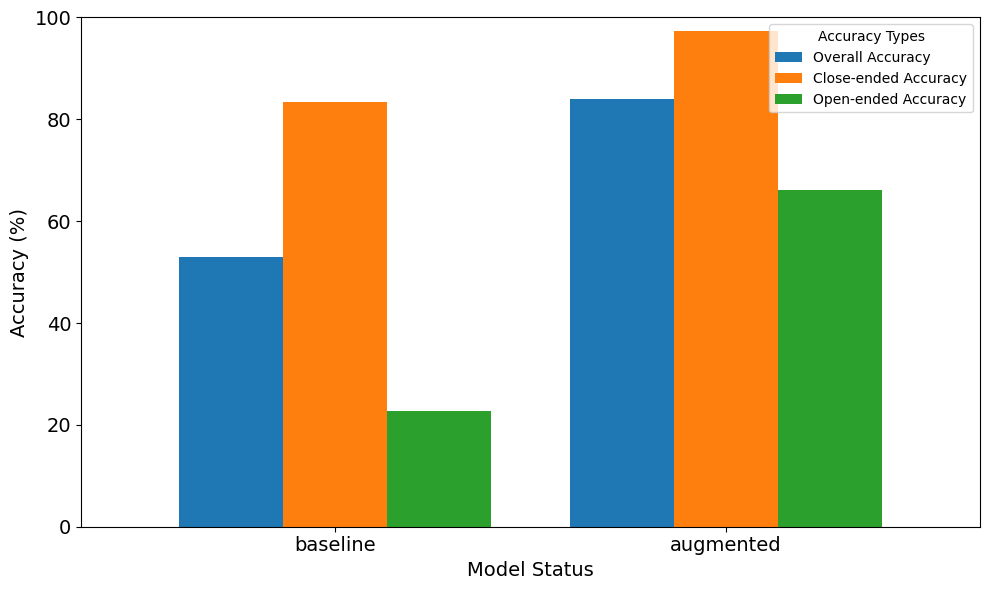
\includegraphics[width=\textwidth]{image/bab4/blip-pathvqa.png}
  \caption{Perbandingan akurasi model BLIP dengan \textit{dataset} PathVQA sebelum dan sesudah dilakukan augmentasi data pertanyaan}
  \label{fig:perbandingan-akurasi-blip-pathvqa}
\end{figure}

\par Lalu, untuk model BLIP yang dilatih dengan \textit{dataset} VQA-RAD juga menghasilkan performa yang lebih baik setelah dilakukan augmentasi data pertanyaan. Hal ini dapat dilihat dari peningkatan nilai akurasi, akurasi \textit{close-ended}, dan akurasi \textit{open-ended} dari \textit{baseline} model yang sebelumnya dilatih tanpa augmentasi data pertanyaan dengan konfigurasi \textit{hyperparameter} \textit{epochs} 15, \textit{batch size} 8, dan \textit{learning rate} $1 \times 10^{-5}$ menghasilkan akurasi 39,73\%, akurasi \textit{close-ended} 61,54\%, dan akurasi \textit{open-ended} 39,64\%. Pada \textit{dataset} VQA-RAD yang telah dilakukan augmentasi data pertanyaan, model BLIP menghasilkan akurasi 82,86\%, akurasi \textit{close-ended} 87,85\%, dan akurasi \textit{open-ended} 76,82\% dengan \textit{hyperparameter} \textit{epochs} 45, \textit{batch size} 8, dan \textit{learning rate} $5 \times 10^{-5}$. Hal ini menunjukkan bahwa nilai akurasi meningkat sebesar 43,13\%, dikarenakan akurasi \textit{close-ended} meningkat sebesar 26,31\% dan akurasi \textit{open-ended} yang juga meningkat sebesar 37,18\%. Pada Gambar \ref{fig:perbandingan-akurasi-blip-vqa-rad} menunjukkan perbandingan \textit{baseline} model dengan model BLIP setelah dilakukan augmentasi data pertanyaan.

\begin{figure}[H]
  \centering
  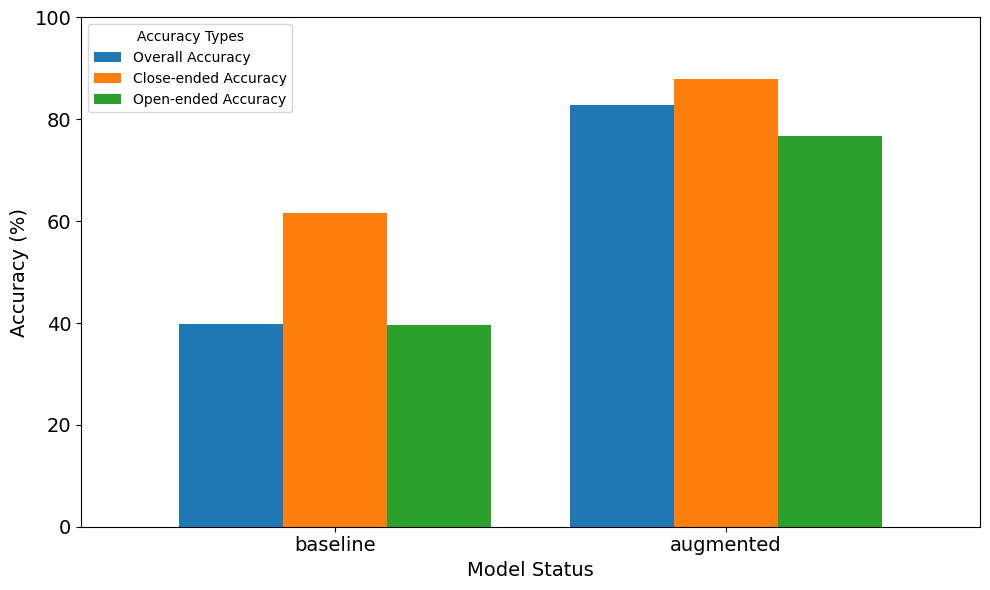
\includegraphics[width=\textwidth]{image/bab4/blip-vqarad.png}
  \caption{Perbandingan akurasi model BLIP dengan \textit{dataset} VQA-RAD sebelum dan sesudah dilakukan augmentasi data pertanyaan}
  \label{fig:perbandingan-akurasi-blip-vqa-rad}
\end{figure}

\par Sedangkan untuk model VGG19-LSTM yang dilatih dengan \textit{dataset} PathVQA tidak menghasilkan performa yang lebih baik setelah dilakukan augmentasi data pertanyaan. Hal ini karena hasil yang didapatkan tidak menunjukkan peningkatan nilai akurasi, akurasi \textit{close-ended}, dan akurasi \textit{open-ended} dari \textit{baseline} model yang sebelumnya dilatih tanpa augmentasi data pertanyaan dengan konfigurasi \textit{hyperparameter} \textit{epochs} 15, \textit{batch size} 8, dan \textit{learning rate} $1 \times 10^{-5}$ menghasilkan akurasi 26,96\%, akurasi \textit{close-ended} 43,73\%, dan akurasi \textit{open-ended} 10,16\%. Pada \textit{dataset} PathVQA yang telah dilakukan augmentasi data pertanyaan, model VGG19-LSTM menghasilkan akurasi 25,87\%, akurasi \textit{close-ended} 41,73\%, dan akurasi \textit{open-ended} 0,10\% dengan \textit{hyperparameter} \textit{epochs} 15, \textit{batch size} 8, dan \textit{learning rate} $1 \times 10^{-5}$. Hal ini menunjukkan bahwa adanya penurunan nilai akurasi sebesar 1,09\%, dikarenakan akurasi \textit{close-ended} yang mengalami penurunan sebesar 2,00\% dan akurasi \textit{open-ended} yang mengalami penurunan sebesar 10,06\%. Lalu, pada saat mengevaluasi dengan BLEU pada pertanyaan \textit{open-ended} menunjukkan bahwa kemampuan model VGG19-LSTM yang dilatih dengan \textit{dataset} PathVQA hampir tidak dapat dipahami dalam mengevaluasi jawaban untuk kata tunggal, pasangan dua kata yang berurutan, dan frasa tiga kata yang berurutan, dikarenakan nilai BLEU-1, BLEU-2, dan BLEU-3 yang didapat adalah 0,19, 0,06, dan 0,05. Pada Gambar \ref{fig:perbandingan-akurasi-vgg19-lstm-pathvqa} menunjukkan perbandingan \textit{baseline} model dengan model VGG19-LSTM setelah dilakukan augmentasi data pertanyaan.

\begin{figure}[H]
  \centering
  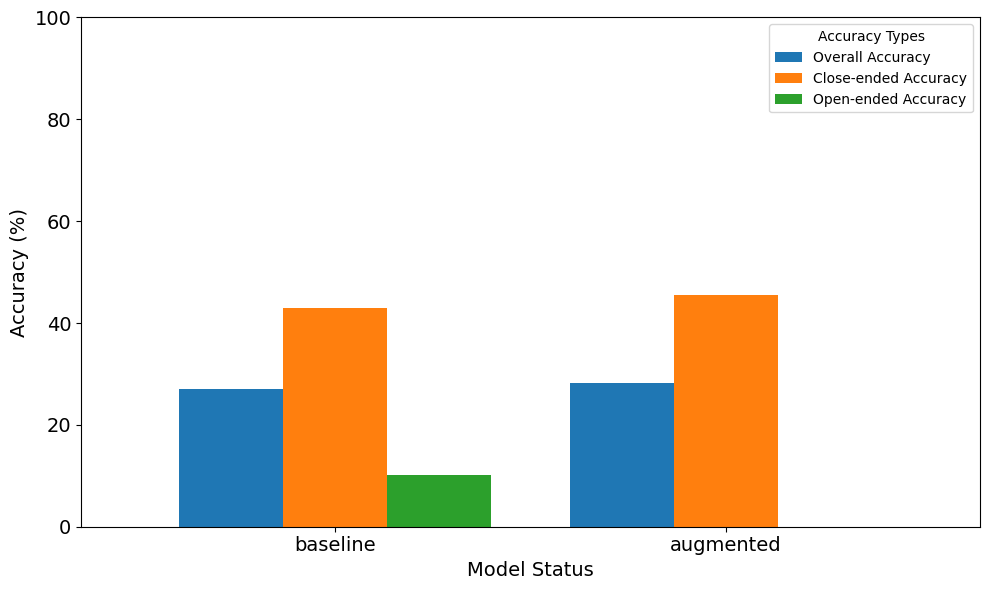
\includegraphics[width=\textwidth]{image/bab4/vgg19-lstm-pathvqa.png}
  \caption{Perbandingan akurasi model VGG19-LSTM dengan \textit{dataset} PathVQA sebelum dan sesudah dilakukan augmentasi data pertanyaan}
  \label{fig:perbandingan-akurasi-vgg19-lstm-pathvqa}
\end{figure}

\par Lalu, untuk model VGG19-LSTM yang dilatih dengan \textit{dataset} VQA-RAD menghasilkan performa yang baik setelah dilakukan augmentasi data pertanyaan. Walaupun hasil yang didapat tidak sebaik model BLIP, namun hasil yang didapat menunjukkan peningkatan performa setelah dilakukan augmentasi data pertanyaan. Hal ini dapat dilihat dari peningkatan nilai akurasi, akurasi \textit{close-ended}, dan akurasi \textit{open-ended} dari \textit{baseline} model yang sebelumnya dilatih tanpa augmentasi data pertanyaan dengan konfigurasi \textit{hyperparameter} \textit{epochs} 15, \textit{batch size} 8, dan \textit{learning rate} $1 \times 10^{-5}$ menghasilkan akurasi 24,44\%, akurasi \textit{close-ended} 43,52\%, dan akurasi \textit{open-ended} 6,84\%. Pada \textit{dataset} VQA-RAD yang telah dilakukan augmentasi data pertanyaan, model VGG19-LSTM menghasilkan akurasi 41,64\%, akurasi \textit{close-ended} 62,40\%, dan akurasi \textit{open-ended} 16,54\% dengan \textit{hyperparameter} \textit{epochs} 15, \textit{batch size} 8, dan \textit{learning rate} $1 \times 10^{-5}$. Hal ini menunjukkan bahwa nilai akurasi meningkat sebesar 17,20\%, dikarenakan akurasi \textit{close-ended} meningkat sebesar 18,88\% dan akurasi \textit{open-ended} yang juga meningkat sebesar 9,70\%. Ketika mengevaluasi dengan BLEU pada pertanyaan \textit{open-ended} menunjukkan bahwa kemampuan model VGG19-LSTM yang dilatih dengan \textit{dataset} VQA-RAD sulit untuk memahami kata tunggal dan dua kata yang berurutan, dikarenakan nilai BLEU-1 dan BLEU-2 yang didapat adalah 17,17 dan 10,5. Sementara itu, model VGG19-LSTM ini juga hampir tidak mampu memahami frasa tiga kata yang berurutan, hal ini dikarenakan nilai BLEU-3 yang tercatat sebesar 7,39. Pada Gambar \ref{fig:perbandingan-akurasi-vgg19-lstm-vqa-rad} menunjukkan perbandingan \textit{baseline} model dengan model VGG19-LSTM setelah dilakukan augmentasi data pertanyaan.

\begin{figure}[H]
  \centering
  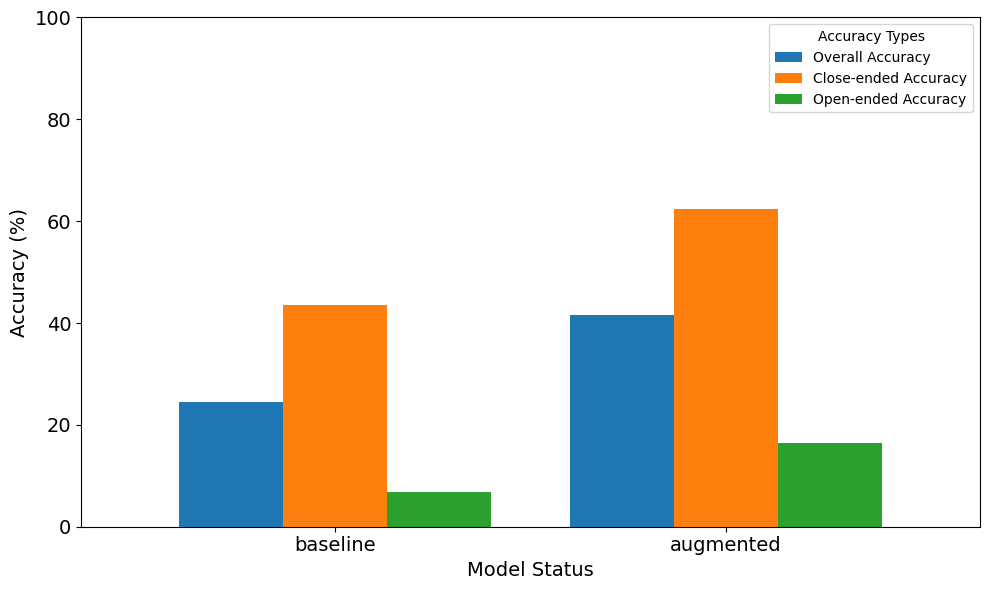
\includegraphics[width=\textwidth]{image/bab4/vgg19-lstm-vqarad.png}
  \caption{Perbandingan akurasi model VGG19-LSTM dengan \textit{dataset} VQA-RAD sebelum dan sesudah dilakukan augmentasi data pertanyaan}
  \label{fig:perbandingan-akurasi-vgg19-lstm-vqa-rad}
\end{figure}


\par Dari semua eksperimen yang sudah dilakukan, dapat dilihat bahwa nilai akurasi untuk pertanyaan \textit{close-ended} lebih tinggi dibandingkan dengan pertanyaan \textit{open-ended}. Hal ini bisa saja disebabkan dikarenakan pertanyaan \textit{close-ended} memiliki distribusi yang lebih banyak dibandingkan dengan pertanyaan \textit{open-ended}. Lalu, dapat disimpulkan juga bahwa model BLIP yang dilatih dengan \textit{dataset} PathVQA dan VQA-RAD menghasilkan performa yang lebih baik dibandingkan dengan model VGG19-LSTM. Hal ini menunjukkan bahwa model BLIP yang dilatih dengan \textit{dataset} PathVQA dan VQA-RAD dapat digunakan untuk menjawab pertanyaan berdasarkan citra patologi dan radiologi dengan performa yang lebih baik dibandingkan dengan model VGG19-LSTM.

\section{Pengembangan Sistem Medis Cerdas Berbasis Web}

\par Pada pengembangan sistem medis cerdas berbasis web ini meliputi tiga halaman, yaitu halaman utama, halaman untuk menjawab pertanyaan berdasarkan citra patologi, dan halaman untuk menjawab pertanyaan berdasarkan citra radiologi. Pada halaman utama, pengguna dapat memilih jenis citra yang diinginkan, yaitu citra patologi atau citra radiologi. Halaman utama ini dapat dilihat pada Gambar \ref{fig:halaman-utama}. Halaman utama ini akan mengarahkan pengguna ke halaman untuk menjawab pertanyaan berdasarkan citra patologi atau radiologi sesuai dengan pilihan pengguna.

\begin{figure}[H]
    \centering
    \label{fig:halaman-utama}
    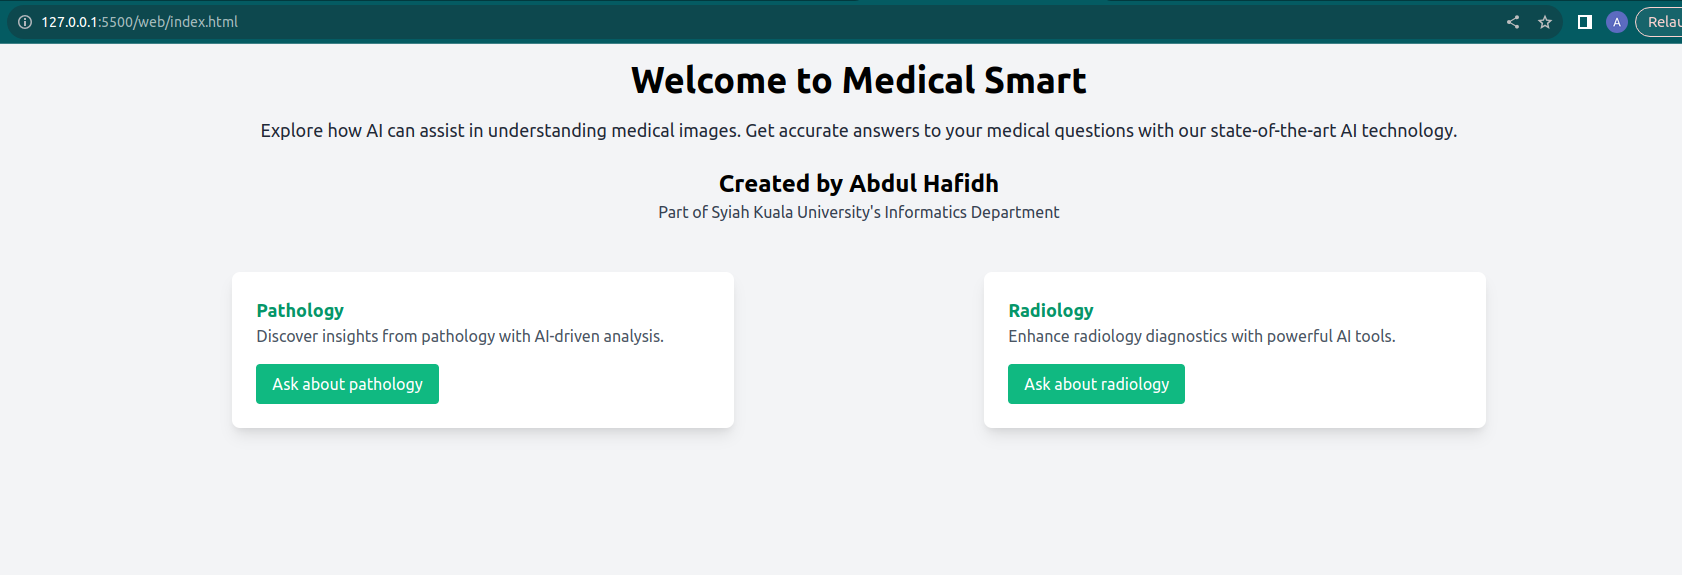
\includegraphics[width=\textwidth, height = 7cm]{image/bab4/halaman_utama.png}
    \caption{Halaman utama sistem medis cerdas berbasis web}
    \label{fig:halaman-utama}
\end{figure}

\par Pada halaman untuk menjawab pertanyaan berdasarkan citra patologi, pengguna dapat mengunggah citra patologi dan menuliskan pertanyaan yang ingin diajukan. Halaman ini akan menampilkan jawaban dari pertanyaan yang diajukan berdasarkan citra patologi yang diunggah. Halaman ini dapat dilihat pada Gambar \ref{fig:halaman-patologi}.

\begin{figure}[H]
  \centering
  \label{fig:halaman-patologi}
  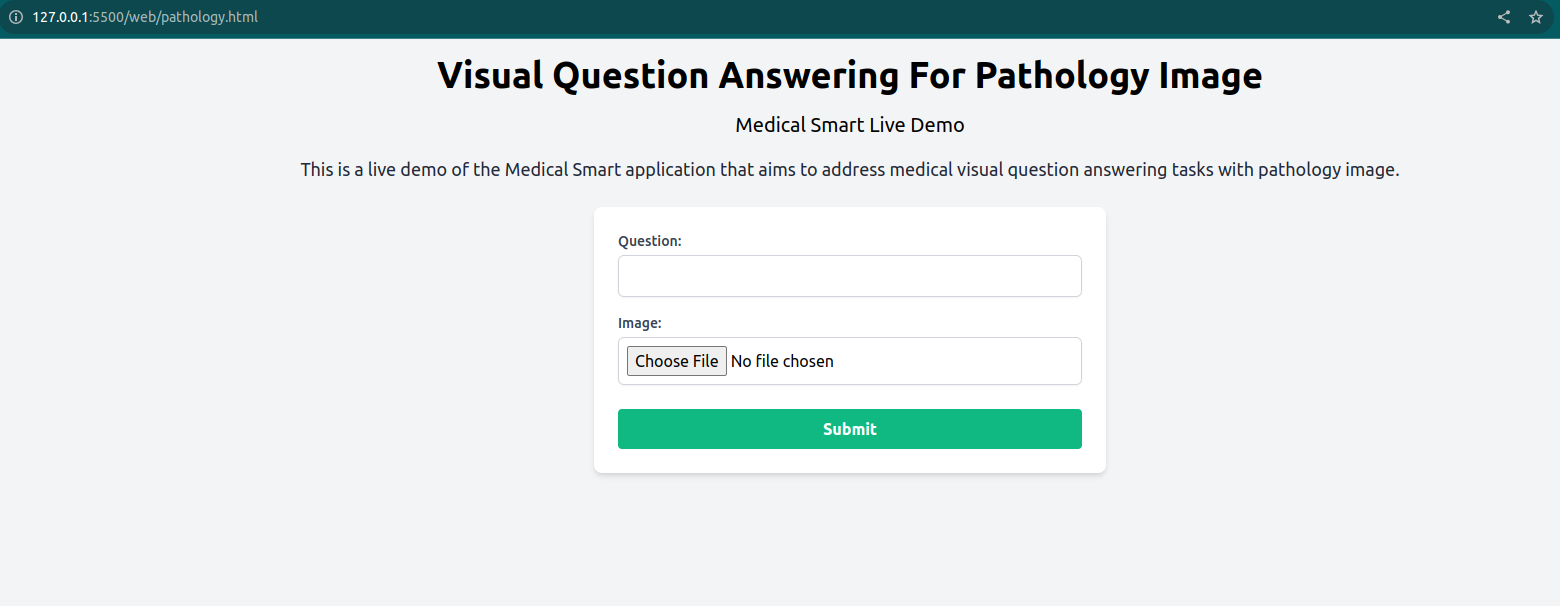
\includegraphics[width=\textwidth, height = 7cm]{image/bab4/halaman_patologi.png}
  \caption{Halaman untuk menjawab pertanyaan berdasarkan citra patologi}
  \label{fig:halaman-patologi}
\end{figure}

Pada halaman untuk menjawab pertanyaan berdasarkan citra radiologi, pengguna dapat mengunggah citra radiologi dan menuliskan pertanyaan yang ingin diajukan. Halaman ini akan menampilkan jawaban dari pertanyaan yang diajukan berdasarkan citra radiologi yang diunggah. Halaman ini dapat dilihat pada Gambar \ref{fig:halaman-radiologi}.

\begin{figure}[H]
  \centering
  \label{fig:halaman-radiologi}
  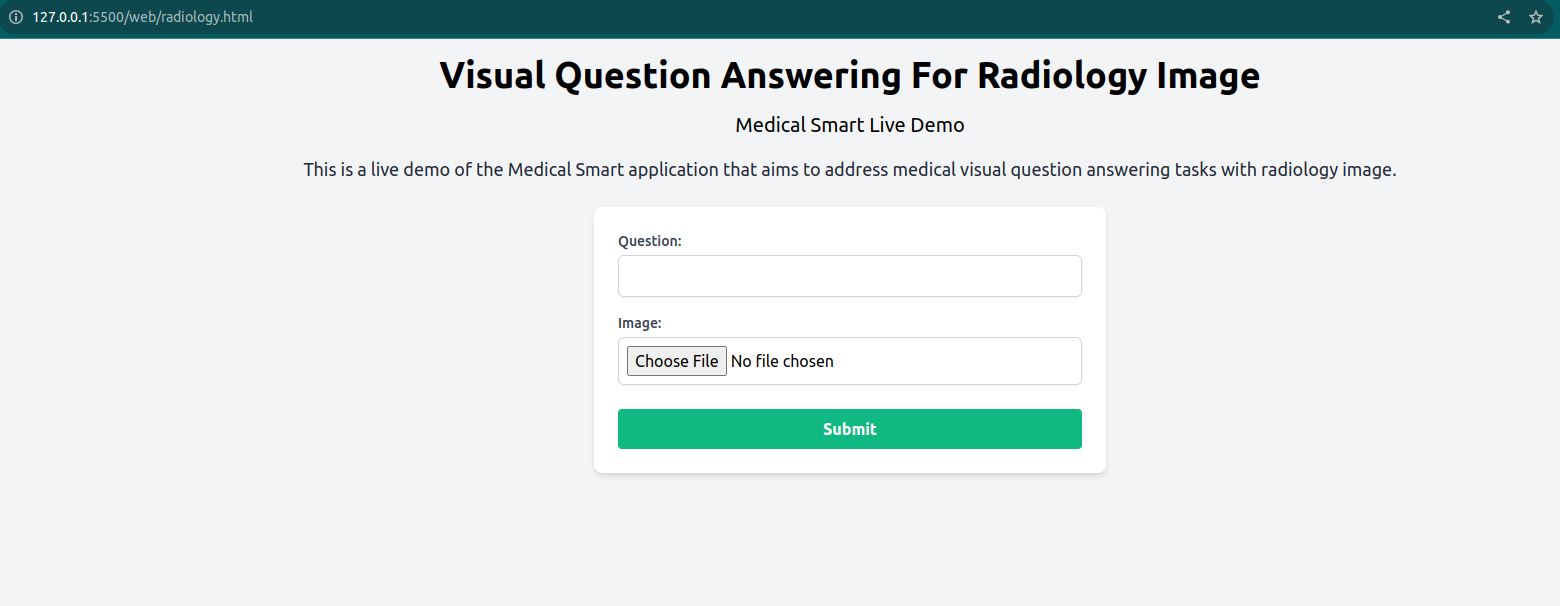
\includegraphics[width=\textwidth]{image/bab4/halaman_radiologi.png}
  \caption{Halaman untuk menjawab pertanyaan berdasarkan citra radiologi}
  \label{fig:halaman-radiologi}
\end{figure}

\par Model yang digunakan dalam sistem ini adalah model BLIP, dikarenakan model BLIP yang dilatih dengan \textit{dataset} PathVQA dan VQA-RAD yang telah dilakukan augmentasi data pertanyaan menghasilkan performa yang lebih baik dibandingkan dengan model VGG19-LSTM. Model BLIP yang dilatih dengan \textit{dataset} PathVQA yang telah dilakukan augmentasi data pertanyaan dengan \textit{hyperparameter} \textit{epochs} 15, \textit{batch size} 8, dan \textit{learning rate} $1 \times 10^{-5}$ akan digunakan untuk menjawab pertanyaan berdasarkan citra patologi. Model BLIP yang dilatih dengan \textit{dataset} VQA-RAD yang telah dilakukan augmentasi data pertanyaan dengan \textit{hyperparameter} \textit{epochs} 45, \textit{batch size} 8, dan \textit{learning rate} $5 \times 10^{-5}$ akan digunakan untuk menjawab pertanyaan berdasarkan citra radiologi.

\par Setelah memilih model yang akan digunakan, disini akan dilakukan tahap kuantisasi model yang bertujuan dalam memperkecil ukuran model tanpa mengorbankan performa dan mempercepat proses inferensi. Pada tahap kuantisasi model ini akan dilakukan dengan menggunakan metode \textit{dynamic quantization} yang disediakan oleh \textit{framework} PyTorch untuk tahapan kuantisasi ini. Pada Tabel \ref{tab:spesifikasi-model} menunjukkan spesifikasi model BLIP sebelum dan sesudah dikuantisasi pada \textit{dataset} PathVQA dan VQA-RAD untuk membandingkan ukuran model dan rata-rata waktu inferensi.

% Please add the following required packages to your document preamble:
% \usepackage{multirow}
\begin{table}[H]
  \centering
  \caption{Spesifikasi model BLIP sebelum dan sesudah dikuantisasi}
  \label{tab:spesifikasi-model}
  \begin{tabular}{|l|l|l|l|}
  \hline
  \textit{\textbf{Dataset}} & \textbf{Status} & \textbf{\begin{tabular}[c]{@{}l@{}}Ukuran \\ model\end{tabular}} & \textbf{\begin{tabular}[c]{@{}l@{}}Rata-rata\\ waktu inferensi\end{tabular}} \\ \hline
  \multirow{2}{*}{PathVQA} & Tidak dikuantisasi & 1467,73 MB & 0,24 detik \\ \cline{2-4} 
   & Sudah dikuantisasi & 508,21 MB & 0,20 detik \\ \hline
  \multirow{2}{*}{VQA-RAD} & Tidak dikuantisasi & 1467,73 MB & 0,21 detik \\ \cline{2-4} 
   & Sudah dikuantisasi & 508,20 MB & 0,17 detik \\ \hline
  \end{tabular}
\end{table}

\par Pada proses pengembangan \textit{backend} pada sistem ini menggunakan \textit{framework} FastAPI untuk dilakukan \textit{deploy} model yang telah dikuantisasi menjadi sebuah API. Disini dipilih model yang telah dikuantisasi karena ukuran model yang lebih kecil dan rata-rata waktu inferensi yang lebih cepat dibandingkan dengan model yang tidak dikuantisasi sesuai dengan Tabel \ref{tab:spesifikasi-model}. Tabel \ref{tab:daftar-endpoint} menunjukkan daftar API \textit{endpoint} pada sistem medis cerdas berbasis web yang digunakan untuk menjawab pertanyaan berdasarkan citra patologi dan radiologi.


% Please add the following required packages to your document preamble:
% \usepackage{multirow}
% \usepackage{graphicx}
\begin{table}[H]
  \centering
  \caption{Daftar API \textit{endpoint} pada sistem medis cerdas berbasis web}
  \label{tab:daftar-endpoint}
  \resizebox{\columnwidth}{!}{%
  \begin{tabular}{|r|l|l|l|}
  \hline
  \multicolumn{1}{|l|}{\textbf{No}} & \textit{\textbf{Method}} & \textit{\textbf{Endpoint}} & \textbf{Deskripsi} \\ \hline
  1 & \multirow{2}{*}{POST} & /predict/pathology & Menjawab pertanyaan berdasarkan citra patologi \\ \cline{1-1} \cline{3-4} 
  2 &  & /predict/radiology & Menjawab pertanyaan berdasarkan citra radiologi \\ \hline
  \end{tabular}%
  }
  \end{table}

  Tabel \ref{tab:daftar-endpoint} memaparkan daftar API \textit{endpoint} pada sistem medis cerdas berbasis web, yang dirancang untuk menjawab pertanyaan yang berkaitan dengan citra patologi dan radiologi. Kedua \textit{endpoint} ini diakses melalui \textit{method} "POST" dan menerima masukan berupa gambar serta pertanyaan yang diinginkan. Hasil yang diberikan adalah jawaban terhadap pertanyaan tersebut dalam format JSON.

  Dalam konteks sistem ini, ketika pengguna menekan tombol \textit{"Submit"} pada halaman yang ditujukan untuk pertanyaan berbasis citra patologi atau radiologi, akan terjadi \textit{request} ke API \textit{endpoint} yang relevan. Dalam hal ini, \textit{request} ini mengirimkan gambar bersama dengan pertanyaan yang akan dijawab. Setelah \textit{request} diterima oleh \textit{endpoint}, sistem akan melakukan inferensi menggunakan model yang telah dikuantisasi untuk memproses data tersebut. Hasil inferensi berupa lima jawaban yang mungkin benar akan disimpan dalam format JSON, kemudian hasil dari JSON akan dikirim ke halaman pengguna untuk ditampilkan. Pada saat yang sama, hasil jawaban akan diberi \textit{confidence score} yang menunjukkan tingkat keyakinan model terhadap jawaban yang diberikan. 

  \par Setelah pengembangan \textit{backend} selesai, maka proses percobaan untuk menjawab pertanyaan berdasarkan citra patologi dan radiologi dapat dilakukan. Pada uji coba dalam menjawab pertanyaan berdasarkan citra patologi dapat dilihat pada Lampiran 10, sedangkan pada uji coba dalam menjawab pertanyaan berdasarkan citra radiologi dapat dilihat pada Lampiran 11.
  




% Baris ini digunakan untuk membantu dalam melakukan sitasi
% Karena diapit dengan comment, maka baris ini akan diabaikan
% oleh compiler LaTeX.
\begin{comment}
\bibliography{daftar-pustaka}
\end{comment}

\fancyhf{} 
\fancyfoot[R]{\thepage}

%-------------------------------------------------------------------------------
%                            BAB V
%               		KESIMPULAN DAN SARAN
%-------------------------------------------------------------------------------
% \fancyhf{} 
% \fancyfoot[R]{\thepage}
\chapter{KESIMPULAN DAN SARAN}
%\thispagestyle{plain} % Halaman pertama bab menggunakan gaya plain

\section{Kesimpulan}

\par Berdasarkan hasil eksperimen dan perbandingan terhadap arsitektur VGG19-LSTM dan BLIP pada \textit{Visual Question Answering} (VQA) dengan \textit{dataset} PathVQA dan VQA-RAD, diperoleh kesimpulan sebagai berikut:

\begin{enumerate}

    \item Penelitian ini berhasil menerapkan teknik \textit{transfer learning} untuk membangun model VQA dengan menggunakan arsitektur VGG19-LSTM dan BLIP. Arsitektur VGG19-LSTM menggunakan model VGG19 yang telah dilatih pada \textit{dataset} ImageNet untuk ekstraksi fitur citra medis dan model LSTM untuk memproses pertanyaan dari \textit{dataset} PathVQA dan VQA-RAD. Sedangkan BLIP memanfaatkan \textit{pre-trained} model pada tugas VQA yang dilatih dengan \textit{dataset} Visual Genome dan VQA v2.0 untuk memproses citra medis dan pertanyaan dari \textit{dataset} PathVQA dan VQA-RAD.


    \item Model BLIP dengan konfigurasi \textit{hyperparameter}: \textit{epochs} 15, \textit{batch size} 8, dan \textit{learning rate} $1 \times 10^{-5}$ menghasilkan performa terbaik pada \textit{dataset} PathVQA yang telah dilakukan augmentasi pertanyaan dengan menciptakan tujuh variasi pertanyaan yang baru dengan akurasi 83.91\%, akurasi \textit{close-ended} 97,43\%, dan akurasi \textit{open-ended} 66,15\%. Sedangkan untuk nilai BLEU-1, BLEU-2, dan BLEU-3 berturut-turut sebesar 69,6, 49,8, 39,87 untuk pertanyaan \textit{open-ended}.

    \item Model BLIP dengan konfigurasi \textit{hyperparameter}: \textit{epochs} 45, \textit{batch size} 8, dan \textit{learning rate} $5 \times 10^{-5}$ menghasilkan performa terbaik pada \textit{dataset} VQA-RAD yang telah dilakukan augmentasi pertanyaan dengan menciptakan tujuh variasi pertanyaan yang baru dengan akurasi 82,86\%, akurasi \textit{close-ended} 87,85\%, dan akurasi \textit{open-ended} 76,82\%. Sedangkan untuk nilai BLEU-1, BLEU-2, dan BLEU-3 berturut-turut sebesar 80,19, 53,36, 40,47 untuk pertanyaan \textit{open-ended}.

    \item Model VGG19-LSTM menunjukkan keterbatasan dalam menyelesaikan tugas VQA, hal ini terlihat dari hasil eksperimen yang dilakukan pada kedua \textit{dataset} PathVQA dan VQA-RAD. Walaupun telah dilakukan augmentasi data pada kedua \textit{dataset} dan \textit{hyperparameter tuning} pada model VGG19-LSTM, performa model tersebut masih jauh dari nilai yang optimal dibandingkan dengan model BLIP. Oleh karena itu, model BLIP akan diimplementasikan ke dalam sistem medis cerdas berbasis web untuk menjawab pertanyaan berdasarkan citra medis.

    \item Model BLIP yang telah dikuantisasi menunjukkan performa yang lebih baik dibandingkan tanpa kuantisasi. Untuk \textit{dataset} PathVQA, ukuran model pra-kuantisasi adalah 1467.73 MB dengan waktu inferensi 0,24 detik, sedangkan pasca-kuantisasi adalah 508,21 MB dengan waktu inferensi 0,20 detik. Untuk \textit{dataset} VQA-RAD, ukuran model pra-kuantisasi adalah 1467,73 MB dengan waktu inferensi 0,21 detik, dan pasca-kuantisasi adalah 508,20 MB dengan waktu inferensi 0,17 detik. Oleh karena itu, model BLIP yang telah dikuantisasi akan diimplementasikan ke dalam sistem medis cerdas berbasis web agar mempercepat waktu inferensi pada saat proses inferensi berlangsung.



\end{enumerate}


\section{Saran}

\par Berdasarkan kesimpulan yang telah dijelaskan sebelumnya, maka penulis memberikan saran untuk penelitian selanjutnya sebagai berikut:

\begin{enumerate}

    \item Mengimplementasikan metode \textit{embedding} yang lainya seperti \textit{word2vec} atau \textit{fastText} pada model VGG19-LSTM untuk melihat apakah performa model tersebut dapat ditingkatkan.

    \item Melakukan eksperimen dengan menggunakan \textit{pre-trained} model lainya dengan basis \textit{transformer} seperti \textit{Vision Language Transformers} (ViLT), \textit{Vision-and-Language BERT} (ViLBERT), \textit{Learning Cross-Modality Encoder Representations from Transformers} (LXMERT), dan lain-lain pada tugas VQA.

    \item Menerapkan teknik augmentasi data VQA yang lebih kompleks dengan mengimplementasikan model generatif untuk menciptakan gambar dan pertanyaan baru, Sehingga berkemungkinan dapat meningkatkan performa model VQA.    

\end{enumerate}



%-----------------------------------------------------------------------------%

% Baris ini digunakan untuk membantu dalam melakukan sitasi
% Karena diapit dengan comment, maka baris ini akan diabaikan
% oleh compiler LaTeX.
\begin{comment}
\bibliography{daftar-pustaka}
\end{comment}


\fancypagestyle{daftarpustaka}{
    \fancyhf{} % Hapus semua header dan footer yang sudah ada
    \fancyfoot[R]{\thepage} % Letakkan nomor halaman di tengah kepala (center)
    \renewcommand{\headrulewidth}{0pt} % Hapus garis pemisah kepala dengan konten
    \renewcommand{\footrulewidth}{0pt} % Hapus garis pemisah footer dengan konten
}


% Halaman Daftar Pustaka dengan penomoran halaman berada di tengah dan nomor halaman selanjutnya di kanan
\addcontentsline{toc}{chapter}{DAFTAR PUSTAKA}
\begin{onehalfspace}
\begin{spacing}{1}
\pagestyle{daftarpustaka}
\bibliography{daftar-pustaka}
\end{spacing}
%-----------------------------------------------------------------
% Disini akhir masukan Daftar Pustaka
%-----------------------------------------------------------------

%%
% @author Kurnia Saputra
% @version 1.0
% 
% Hanya sebuah pembatas bertuliskan LAMPIRAN ditengah halaman. 
% 

\begin{titlepage}
	\centering 
	\vspace*{6cm}
	\noindent \Huge{LAMPIRAN}
	%\addChapter{LAMPIRAN}
	\addcontentsline{toc}{chapter}{LAMPIRAN}
\end{titlepage}
\addcontentsline{toc}{chapter}{LAMPIRAN}
\titleformat{\section}{\normalfont\bfseries}{\thesection}{1em}{}
% Format judul untuk bagian lampiran
\chapter*{LAMPIRAN}

%\thispagestyle{plain} % Halaman pertama bab menggunakan gaya plain


\newappendix{Lampiran 1. \textit{Layer vision} pada model BLIP}

\begin{figure}[H]
  \centering
  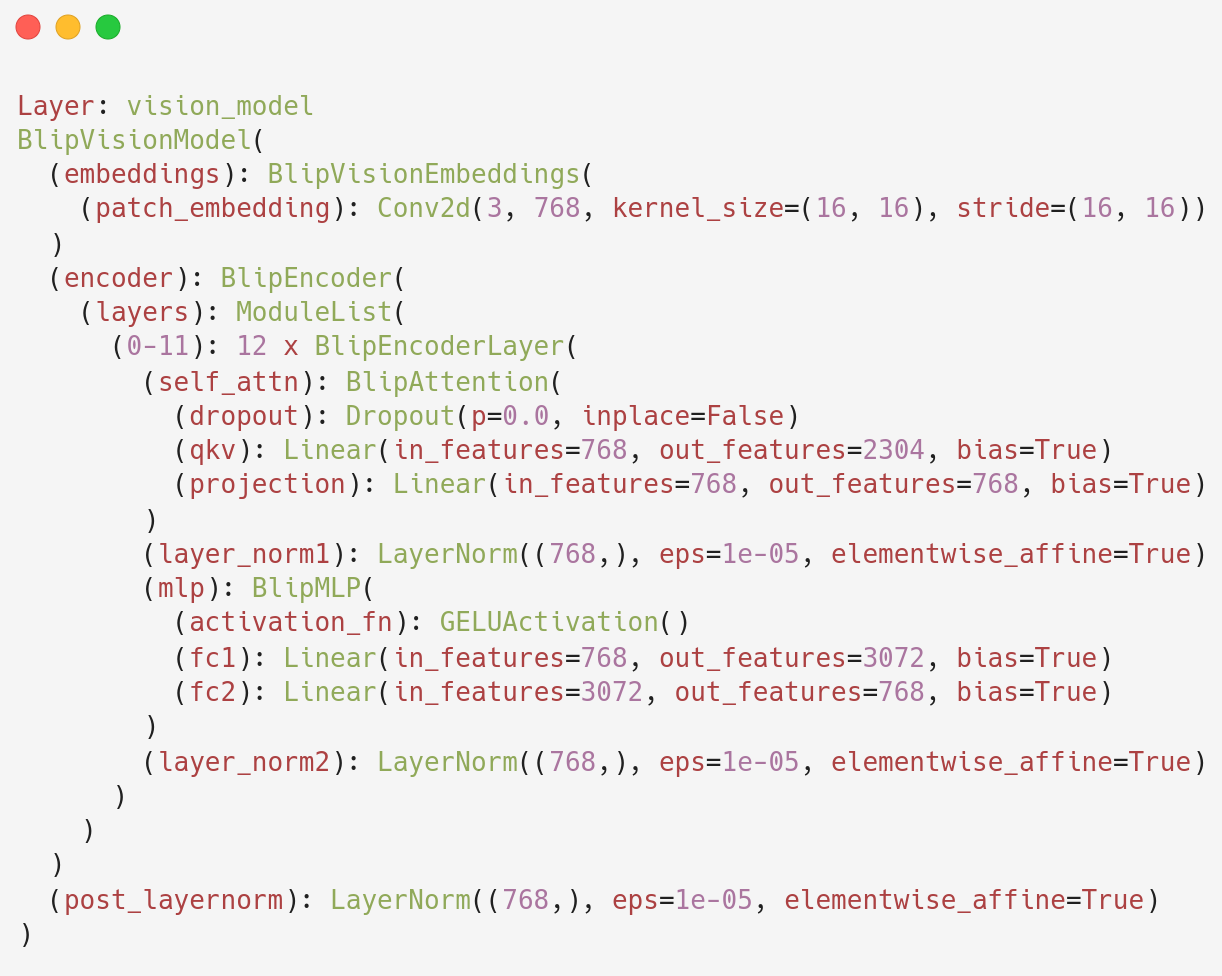
\includegraphics[width=\textwidth, height = 10cm]{image/lampiran/blip-vision-model.png}
  \label{fig:layer-vision-blip}
\end{figure}

\newappendix{Lampiran 2. \textit{Layer text encoder} pada model BLIP}

\begin{figure}[H]
  \centering
  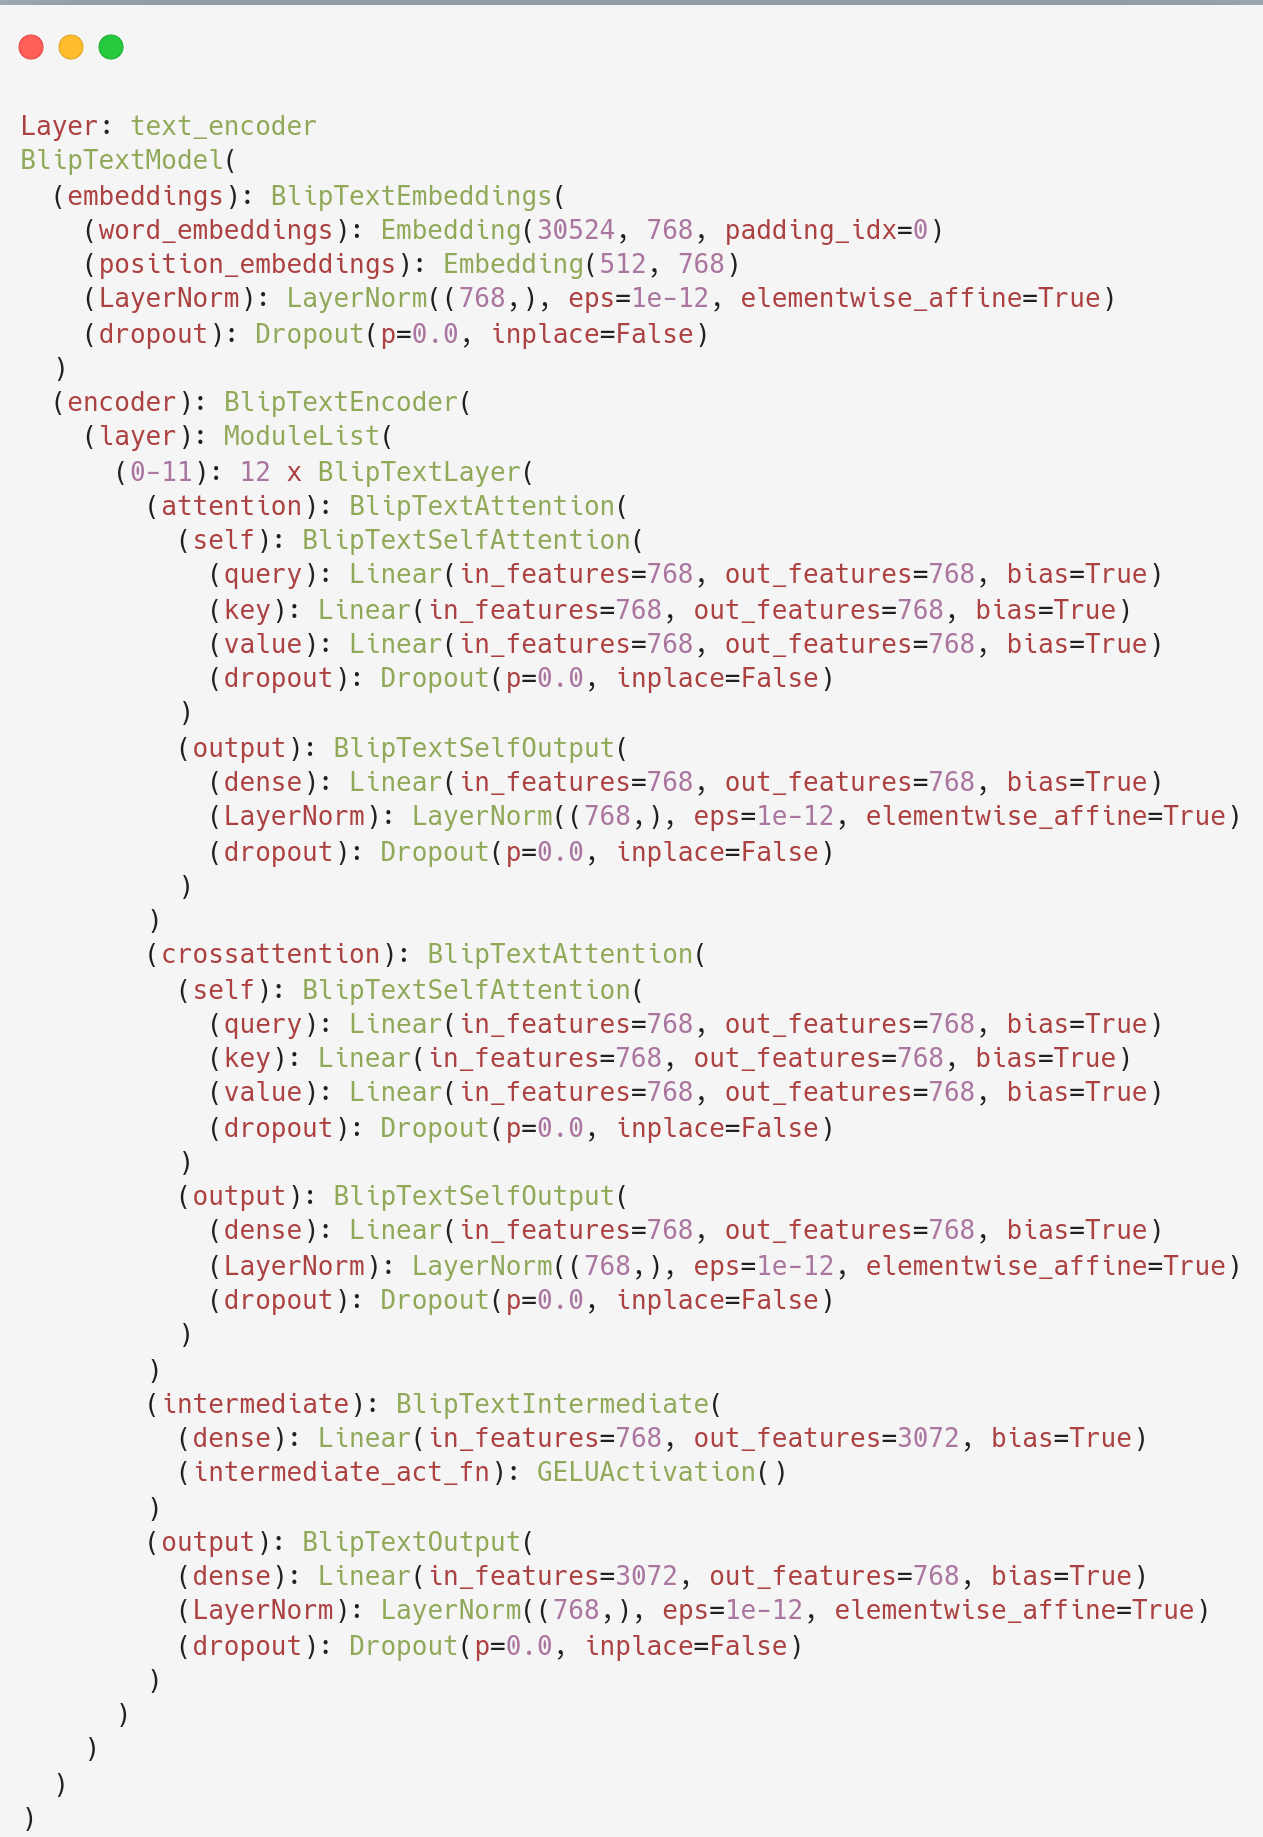
\includegraphics[width=\textwidth]{image/lampiran/blip-text-encoder.png}
  \label{fig:layer-text-encoder-blip}
\end{figure}

\newappendix{Lampiran 3. \textit{Layer text decoder} pada model BLIP}

\begin{figure}[H]
  \centering
  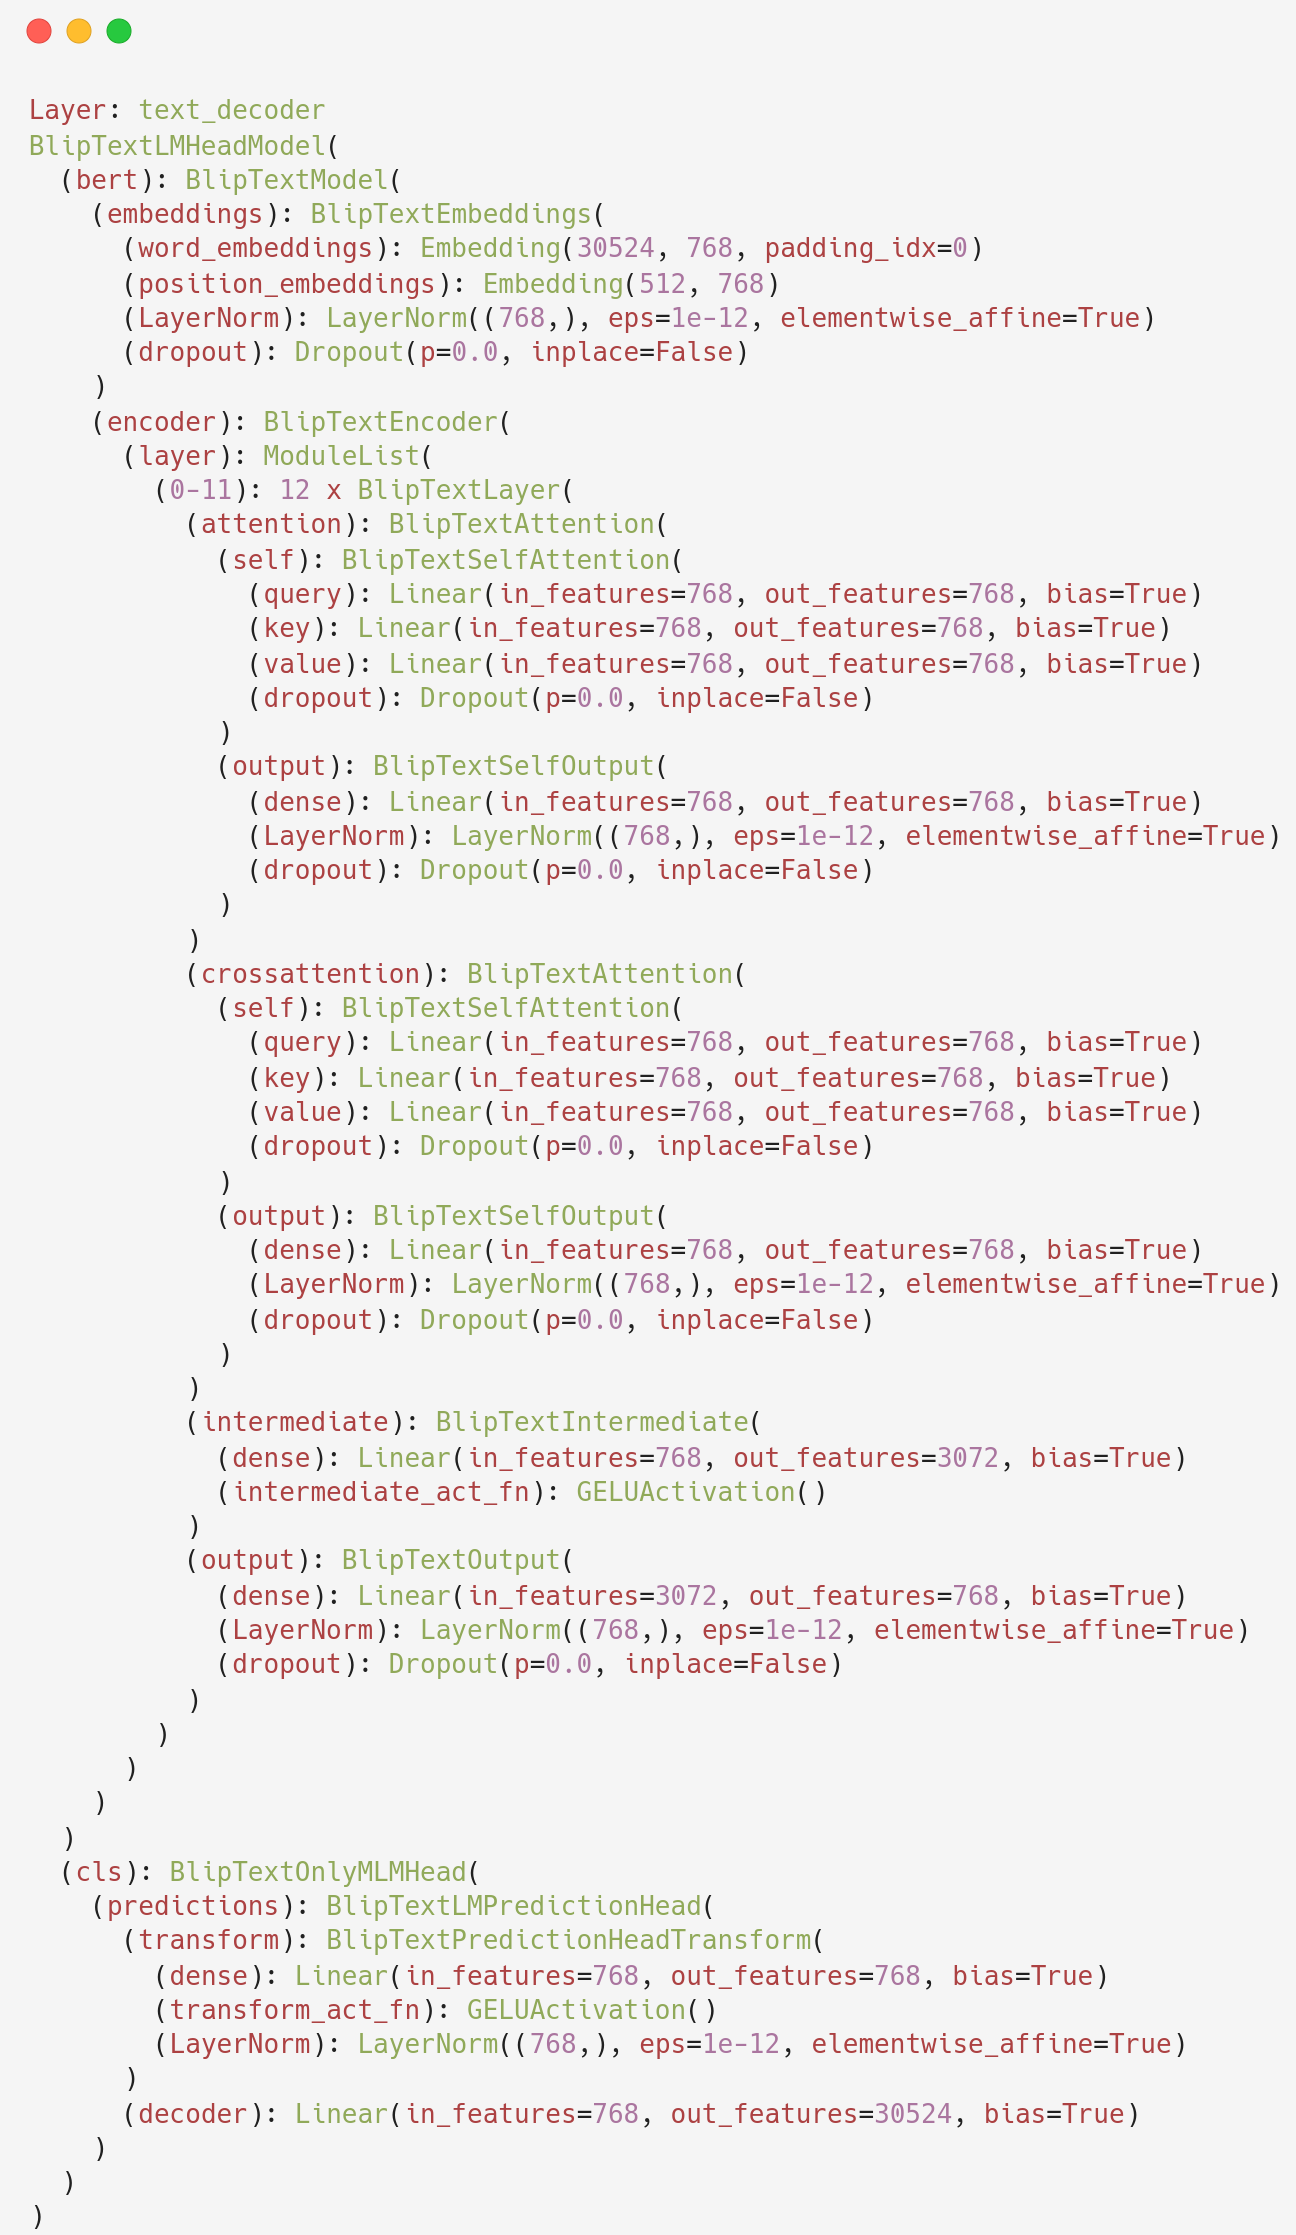
\includegraphics[width=\textwidth, height = 21cm]{image/lampiran/blip-text-decoder.png}
  \label{fig:layer-text-decoder-blip}
\end{figure}


\newappendix{Lampiran 4. Hasil pelatihan dengan VGG19-LSTM untuk pertanyaan \textit{close ended}}

% Please add the following required packages to your document preamble:
% \usepackage{longtable}
% Note: It may be necessary to compile the document several times to get a multi-page table to line up properly
\begin{longtable}[c]{|l|l|l|l|l|l|l|l|}
\hline
\textit{\textbf{Dataset}} &
  \textit{\textbf{Epochs}} &
  \textit{\textbf{\begin{tabular}[c]{@{}l@{}}Batch \\ size\end{tabular}}} &
  \textit{\textbf{\begin{tabular}[c]{@{}l@{}}Learning\\  rate\end{tabular}}} &
  \textbf{Akurasi} &
  \textbf{BLEU-1} &
  \textbf{BLEU-2} &
  \textbf{BLEU-3} \\ \hline
\endfirsthead
%
\endhead
%
PathVQA & 15 & 8  & $1 \times 10^{-5}$ & 43,02\% & 43,02 & 13,60 & 9,41  \\ \hline
PathVQA & 15 & 8  & $5 \times 10^{-5}$ & 53,44\% & 53,45 & 16,90 & 11,69 \\ \hline
PathVQA & 15 & 16 & $1 \times 10^{-5}$ & 44,18\% & 44,18 & 13,97 & 9,67  \\ \hline
PathVQA & 15 & 16 & $5 \times 10^{-5}$ & 51,44\% & 51,44 & 16,27 & 11,25 \\ \hline
PathVQA & 15 & 32 & $1 \times 10^{-5}$ & 47,99\% & 47,99 & 15,18 & 10,50 \\ \hline
PathVQA & 15 & 32 & $5 \times 10^{-5}$ & 45,40\% & 45,40 & 14,36 & 9,93  \\ \hline
PathVQA & 30 & 8  & $1 \times 10^{-5}$ & 39,45\% & 39,45 & 12,48 & 8,63  \\ \hline
PathVQA & 30 & 8  & $5 \times 10^{-5}$ & 48,85\% & 48,85 & 15,45 & 10,69 \\ \hline
PathVQA & 30 & 16 & $1 \times 10^{-5}$ & 52,25\% & 52,25 & 16,52 & 11,43 \\ \hline
PathVQA & 30 & 16 & $5 \times 10^{-5}$ & 49,42\% & 49,42 & 15,63 & 10,81 \\ \hline
PathVQA & 30 & 32 & $1 \times 10^{-5}$ & 38,98\% & 38,98 & 12,33 & 8,53  \\ \hline
PathVQA & 30 & 32 & $5 \times 10^{-5}$ & 49,60\% & 49,60 & 15,69 & 10,85 \\ \hline
PathVQA & 45 & 8  & $1 \times 10^{-5}$ & 48,25\% & 48,25 & 15,26 & 10,56 \\ \hline
PathVQA & 45 & 8  & $5 \times 10^{-5}$ & 48,66\% & 48,66 & 15,39 & 10,65 \\ \hline
PathVQA & 45 & 16 & $1 \times 10^{-5}$ & 38,31\% & 38,32 & 12,12 & 8,39  \\ \hline
PathVQA & 45 & 16 & $5 \times 10^{-5}$ & 51,23\% & 51,24 & 16,20 & 11,21 \\ \hline
PathVQA & 45 & 32 & $1 \times 10^{-5}$ & 49,63\% & 49,65 & 15,70 & 10,86 \\ \hline
PathVQA & 45 & 32 & $5 \times 10^{-5}$ & 14,80\% & 14,80 & 4,68  & 3,24  \\ \hline
VQA-RAD & 15 & 8  & $1 \times 10^{-5}$ & 43,52\% & 43,52 & 13,76 & 9,52  \\ \hline
VQA-RAD & 15 & 8  & $5 \times 10^{-5}$ & 52,85\% & 52,85 & 16,71 & 11,56 \\ \hline
VQA-RAD & 15 & 16 & $1 \times 10^{-5}$ & 47,46\% & 47,46 & 15,01 & 10,38 \\ \hline
VQA-RAD & 15 & 16 & $5 \times 10^{-5}$ & 60,71\% & 60,71 & 19,20 & 13,28 \\ \hline
VQA-RAD & 15 & 32 & $1 \times 10^{-5}$ & 57,27\% & 57,27 & 18,11 & 12,53 \\ \hline
VQA-RAD & 15 & 32 & $5 \times 10^{-5}$ & 62,79\% & 62,79 & 19,86 & 13,74 \\ \hline
VQA-RAD & 30 & 8  & $1 \times 10^{-5}$ & 58,68\% & 58,68 & 18,56 & 12,84 \\ \hline
VQA-RAD & 30 & 8  & $5 \times 10^{-5}$ & 69,05\% & 69,05 & 21,83 & 15,11 \\ \hline
VQA-RAD & 30 & 16 & $1 \times 10^{-5}$ & 60,83\% & 60,83 & 19,24 & 13,31 \\ \hline
VQA-RAD & 30 & 16 & $5 \times 10^{-5}$ & 66,67\% & 66,67 & 21,08 & 14,59 \\ \hline
VQA-RAD & 30 & 32 & $1 \times 10^{-5}$ & 61,02\% & 61,02 & 19,30 & 13,35 \\ \hline
VQA-RAD & 30 & 32 & $5 \times 10^{-5}$ & 57,14\% & 57,14 & 18,07 & 12,50 \\ \hline
VQA-RAD & 45 & 8  & $1 \times 10^{-5}$ & 62,81\% & 62,81 & 19,86 & 13,74 \\ \hline
VQA-RAD & 45 & 8  & $5 \times 10^{-5}$ & 71,05\% & 71,05 & 22,47 & 15,54 \\ \hline
VQA-RAD & 45 & 16 & $1 \times 10^{-5}$ & 57,50\% & 57,50 & 18,18 & 12,58 \\ \hline
VQA-RAD & 45 & 16 & $5 \times 10^{-5}$ & 66,93\% & 66,93 & 21,16 & 14,64 \\ \hline
VQA-RAD & 45 & 32 & $1 \times 10^{-5}$ & 57,98\% & 57,98 & 18,34 & 12,69 \\ \hline
VQA-RAD & 45 & 32 & $5 \times 10^{-5}$ & 68,75\% & 68,75 & 21,74 & 15,04 \\ \hline
\end{longtable}


\newappendix{Lampiran 5. Hasil pelatihan dengan VGG19-LSTM untuk pertanyaan \textit{open ended}}

% Please add the following required packages to your document preamble:
% \usepackage{longtable}
% Note: It may be necessary to compile the document several times to get a multi-page table to line up properly
\begin{longtable}[c]{|l|l|l|l|l|l|l|l|}
  \hline
  \textit{\textbf{Dataset}} &
    \textit{\textbf{Epochs}} &
    \textit{\textbf{\begin{tabular}[c]{@{}l@{}}Batch \\ size\end{tabular}}} &
    \textit{\textbf{\begin{tabular}[c]{@{}l@{}}Learning \\ rate\end{tabular}}} &
    \textbf{Akurasi} &
    \textbf{BLEU-1} &
    \textbf{BLEU-2} &
    \textbf{BLEU-3} \\ \hline
  \endfirsthead
  %
  \endhead
  %
  PathVQA & 15 & 8  & $1 \times 10^{-5}$ & 10,16\% & 10,89 & 3,86  & 2,57  \\ \hline
  PathVQA & 15 & 8  & $5 \times 10^{-5}$ & 19,90\% & 21,41 & 8,01  & 5,38  \\ \hline
  PathVQA & 15 & 16 & $1 \times 10^{-5}$ & 1,29\%  & 1,37  & 0,48  & 0,32  \\ \hline
  PathVQA & 15 & 16 & $5 \times 10^{-5}$ & 18,53\% & 19,95 & 7,96  & 5,23  \\ \hline
  PathVQA & 15 & 32 & $1 \times 10^{-5}$ & 0,43\%  & 0,48  & 0,15  & 0,10  \\ \hline
  PathVQA & 15 & 32 & $5 \times 10^{-5}$ & 15,63\% & 16,67 & 6,25  & 4,01  \\ \hline
  PathVQA & 30 & 8  & $1 \times 10^{-5}$ & 16,17\% & 17,94 & 6,67  & 4,49  \\ \hline
  PathVQA & 30 & 8  & $5 \times 10^{-5}$ & 20,43\% & 22,46 & 9,02  & 5,87  \\ \hline
  PathVQA & 30 & 16 & $1 \times 10^{-5}$ & 14,59\% & 16,22 & 6,49  & 4,29  \\ \hline
  PathVQA & 30 & 16 & $5 \times 10^{-5}$ & 14,48\% & 17,32 & 7,30  & 5,08  \\ \hline
  PathVQA & 30 & 32 & $1 \times 10^{-5}$ & 7,36\%  & 8,01  & 2,83  & 1,88  \\ \hline
  PathVQA & 30 & 32 & $5 \times 10^{-5}$ & 16,49\% & 18,69 & 7,56  & 5,15  \\ \hline
  PathVQA & 45 & 8  & $1 \times 10^{-5}$ & 15,46\% & 18,06 & 7,43  & 5,09  \\ \hline
  PathVQA & 45 & 8  & $5 \times 10^{-5}$ & 22,15\% & 24,28 & 10,02 & 6,81  \\ \hline
  PathVQA & 45 & 16 & $1 \times 10^{-5}$ & 17,61\% & 19,65 & 7,86  & 5,14  \\ \hline
  PathVQA & 45 & 16 & $5 \times 10^{-5}$ & 19,77\% & 22,32 & 9,63  & 6,72  \\ \hline
  PathVQA & 45 & 32 & $1 \times 10^{-5}$ & 13,72\% & 15,74 & 6,51  & 4,31  \\ \hline
  PathVQA & 45 & 32 & $5 \times 10^{-5}$ & 1,95\%  & 2,65  & 1,25  & 0,88  \\ \hline
  VQA-RAD & 15 & 8  & $1 \times 10^{-5}$ & 6,84\%  & 7,87  & 5,53  & 4,27  \\ \hline
  VQA-RAD & 15 & 8  & $5 \times 10^{-5}$ & 15,69\% & 17,60 & 10,74 & 7,37  \\ \hline
  VQA-RAD & 15 & 16 & $1 \times 10^{-5}$ & 5,61\%  & 6,30  & 4,10  & 2,75  \\ \hline
  VQA-RAD & 15 & 16 & $5 \times 10^{-5}$ & 8,85\%  & 10,27 & 7,01  & 4,19  \\ \hline
  VQA-RAD & 15 & 32 & $1 \times 10^{-5}$ & 1,74\%  & 1,90  & 1,90  & 1,44  \\ \hline
  VQA-RAD & 15 & 32 & $5 \times 10^{-5}$ & 5,21\%  & 5,79  & 3,26  & 2,34  \\ \hline
  VQA-RAD & 30 & 8  & $1 \times 10^{-5}$ & 10,58\% & 12,55 & 8,99  & 7,25  \\ \hline
  VQA-RAD & 30 & 8  & $5 \times 10^{-5}$ & 18,18\% & 20,17 & 14,34 & 11,32 \\ \hline
  VQA-RAD & 30 & 16 & $1 \times 10^{-5}$ & 3,81\%  & 5,11  & 3,18  & 2,92  \\ \hline
  VQA-RAD & 30 & 16 & $5 \times 10^{-5}$ & 6,31\%  & 8,17  & 5,68  & 3,91  \\ \hline
  VQA-RAD & 30 & 32 & $1 \times 10^{-5}$ & 5,61\%  & 6,17  & 6,17  & 4,88  \\ \hline
  VQA-RAD & 30 & 32 & $5 \times 10^{-5}$ & 7,96\%  & 9,37  & 6,01  & 4,65  \\ \hline
  VQA-RAD & 45 & 8  & $1 \times 10^{-5}$ & 11,54\% & 12,26 & 7,23  & 5,51  \\ \hline
  VQA-RAD & 45 & 8  & $5 \times 10^{-5}$ & 11,71\% & 13,08 & 7,45  & 4,74  \\ \hline
  VQA-RAD & 45 & 16 & $1 \times 10^{-5}$ & 11,43\% & 13,19 & 10,84 & 6,99  \\ \hline
  VQA-RAD & 45 & 16 & $5 \times 10^{-5}$ & 18,37\% & 20,69 & 16,69 & 11,29 \\ \hline
  VQA-RAD & 45 & 32 & $1 \times 10^{-5}$ & 3,77\%  & 4,97  & 3,80  & 2,97  \\ \hline
  VQA-RAD & 45 & 32 & $5 \times 10^{-5}$ & 14,16\% & 15,16 & 11,64 & 7,85  \\ \hline
  \end{longtable}

\newappendix{Lampiran 6. Hasil pelatihan dengan VGG19-LSTM untuk semua pertanyaan}

% Please add the following required packages to your document preamble:
% \usepackage{longtable}
% Note: It may be necessary to compile the document several times to get a multi-page table to line up properly
\begin{longtable}[c]{|l|l|l|l|l|l|l|l|}
  \hline
  \textit{\textbf{Dataset}} &
    \textit{\textbf{Epochs}} &
    \textit{\textbf{\begin{tabular}[c]{@{}l@{}}Batch \\ size\end{tabular}}} &
    \textit{\textbf{\begin{tabular}[c]{@{}l@{}}Learning \\ rate\end{tabular}}} &
    \textbf{Akurasi} &
    \textbf{BLEU-1} &
    \textbf{BLEU-2} &
    \textbf{BLEU-3} \\ \hline
  \endfirsthead
  %
  \endhead
  %
  PathVQA & 15 & 8  & $1 \times 10^{-5}$ & 26,96\% & 27,32 & 8,84  & 6,07  \\ \hline
  PathVQA & 15 & 8  & $5 \times 10^{-5}$ & 37,07\% & 37,81 & 12,56 & 8,61  \\ \hline
  PathVQA & 15 & 16 & $1 \times 10^{-5}$ & 22,73\% & 22,77 & 7,23  & 4,99  \\ \hline
  PathVQA & 15 & 16 & $5 \times 10^{-5}$ & 34,68\% & 35,41 & 12,04 & 8,19  \\ \hline
  PathVQA & 15 & 32 & $1 \times 10^{-5}$ & 24,39\% & 24,41 & 7,72  & 5,34  \\ \hline
  PathVQA & 15 & 32 & $5 \times 10^{-5}$ & 30,70\% & 31,21 & 10,35 & 7,01  \\ \hline
  PathVQA & 30 & 8  & $1 \times 10^{-5}$ & 27,76\% & 28,65 & 9,56  & 6,55  \\ \hline
  PathVQA & 30 & 8  & $5 \times 10^{-5}$ & 34,41\% & 35,44 & 12,18 & 8,24  \\ \hline
  PathVQA & 30 & 16 & $1 \times 10^{-5}$ & 33,03\% & 33,86 & 11,40 & 7,79  \\ \hline
  PathVQA & 30 & 16 & $5 \times 10^{-5}$ & 31,89\% & 33,32 & 11,45 & 7,94  \\ \hline
  PathVQA & 30 & 32 & $1 \times 10^{-5}$ & 23,19\% & 23,51 & 7,59  & 5,21  \\ \hline
  PathVQA & 30 & 32 & $5 \times 10^{-5}$ & 33,18\% & 34,27 & 11,65 & 8,02  \\ \hline
  PathVQA & 45 & 8  & $1 \times 10^{-5}$ & 31,80\% & 33,11 & 11,33 & 7,82  \\ \hline
  PathVQA & 45 & 8  & $5 \times 10^{-5}$ & 35,20\% & 36,28 & 12,67 & 8,70  \\ \hline
  PathVQA & 45 & 16 & $1 \times 10^{-5}$ & 27,97\% & 28,99 & 9,99  & 6,77  \\ \hline
  PathVQA & 45 & 16 & $5 \times 10^{-5}$ & 35,39\% & 36,67 & 12,89 & 8,95  \\ \hline
  PathVQA & 45 & 32 & $1 \times 10^{-5}$ & 31,43\% & 32,46 & 11,04 & 7,54  \\ \hline
  PathVQA & 45 & 32 & $5 \times 10^{-5}$ & 8,12\%  & 8,48  & 2,90  & 2,01  \\ \hline
  VQA-RAD & 15 & 8  & $1 \times 10^{-5}$ & 24,44\% & 24,98 & 9,48  & 6,79  \\ \hline
  VQA-RAD & 15 & 8  & $5 \times 10^{-5}$ & 36,00\% & 36,87 & 14,00 & 9,66  \\ \hline
  VQA-RAD & 15 & 16 & $1 \times 10^{-5}$ & 27,56\% & 27,89 & 9,82  & 6,75  \\ \hline
  VQA-RAD & 15 & 16 & $5 \times 10^{-5}$ & 34,67\% & 35,38 & 13,08 & 8,71  \\ \hline
  VQA-RAD & 15 & 32 & $1 \times 10^{-5}$ & 28,89\% & 28,97 & 9,83  & 6,86  \\ \hline
  VQA-RAD & 15 & 32 & $5 \times 10^{-5}$ & 38,22\% & 38,47 & 12,77 & 8,87  \\ \hline
  VQA-RAD & 30 & 8  & $1 \times 10^{-5}$ & 36,44\% & 37,36 & 14,13 & 10,26 \\ \hline
  VQA-RAD & 30 & 8  & $5 \times 10^{-5}$ & 46,67\% & 47,54 & 18,54 & 13,44 \\ \hline
  VQA-RAD & 30 & 16 & $1 \times 10^{-5}$ & 34,22\% & 34,83 & 11,74 & 8,46  \\ \hline
  VQA-RAD & 30 & 16 & $5 \times 10^{-5}$ & 36,89\% & 37,81 & 13,48 & 9,32  \\ \hline
  VQA-RAD & 30 & 32 & $1 \times 10^{-5}$ & 34,67\% & 34,94 & 13,06 & 9,32  \\ \hline
  VQA-RAD & 30 & 32 & $5 \times 10^{-5}$ & 32,44\% & 33,15 & 12,01 & 8,56  \\ \hline
  VQA-RAD & 45 & 8  & $1 \times 10^{-5}$ & 39,11\% & 39,45 & 14,03 & 9,94  \\ \hline
  VQA-RAD & 45 & 8  & $5 \times 10^{-5}$ & 41,78\% & 42,45 & 15,06 & 10,21 \\ \hline
  VQA-RAD & 45 & 16 & $1 \times 10^{-5}$ & 36,00\% & 36,82 & 14,76 & 9,97  \\ \hline
  VQA-RAD & 45 & 16 & $5 \times 10^{-5}$ & 45,78\% & 46,79 & 19,22 & 13,18 \\ \hline
  VQA-RAD & 45 & 32 & $1 \times 10^{-5}$ & 32,44\% & 33,01 & 11,49 & 8,11  \\ \hline
  VQA-RAD & 45 & 32 & $5 \times 10^{-5}$ & 41,33\% & 41,83 & 16,67 & 11,43 \\ \hline
  \end{longtable}

\newappendix{Lampiran 7. Hasil pelatihan dengan BLIP untuk pertanyaan \textit{close ended}}

% Please add the following required packages to your document preamble:
% \usepackage{longtable}
% Note: It may be necessary to compile the document several times to get a multi-page table to line up properly
\begin{longtable}[c]{|l|l|l|l|l|l|l|l|}
    \hline
    \textit{\textbf{Dataset}} &
      \textit{\textbf{Epochs}} &
      \textit{\textbf{\begin{tabular}[c]{@{}l@{}}Batch \\ size\end{tabular}}} &
      \textit{\textbf{\begin{tabular}[c]{@{}l@{}}Learning \\ rate\end{tabular}}} &
      \textbf{Akurasi} &
      \textbf{BLEU-1} &
      \textbf{BLEU-2} &
      \textbf{BLEU-3} \\ \hline
    \endfirsthead
    %
    \endhead
    %
    PathVQA & 15 & 8  & $1 \times 10^{-5}$ & 83,44\% & 83,44 & 26,38 & 18,25 \\ \hline
    PathVQA & 15 & 8  & $5 \times 10^{-5}$ & 49,27\% & 49,27 & 15,58 & 10,78 \\ \hline
    PathVQA & 15 & 16 & $1 \times 10^{-5}$ & 72,38\% & 72,38 & 22,89 & 15,83 \\ \hline
    PathVQA & 15 & 16 & $5 \times 10^{-5}$ & 82,85\% & 82,85 & 26,20 & 18,13 \\ \hline
    PathVQA & 15 & 32 & $1 \times 10^{-5}$ & 64,24\% & 64,24 & 20,32 & 14,05 \\ \hline
    PathVQA & 15 & 32 & $5 \times 10^{-5}$ & 79,25\% & 79,25 & 25,06 & 17,34 \\ \hline
    PathVQA & 30 & 8  & $1 \times 10^{-5}$ & 77,15\% & 77,15 & 24,40 & 16,88 \\ \hline
    PathVQA & 30 & 8  & $5 \times 10^{-5}$ & 75,46\% & 75,46 & 23,86 & 16,51 \\ \hline
    PathVQA & 30 & 16 & $1 \times 10^{-5}$ & 74,43\% & 74,43 & 23,54 & 16,28 \\ \hline
    PathVQA & 30 & 16 & $5 \times 10^{-5}$ & 71,00\% & 71,00 & 22,45 & 15,53 \\ \hline
    PathVQA & 30 & 32 & $1 \times 10^{-5}$ & 76,11\% & 76,11 & 24,07 & 16,65 \\ \hline
    PathVQA & 30 & 32 & $5 \times 10^{-5}$ & 86,00\% & 86,00 & 27,20 & 18,82 \\ \hline
    PathVQA & 45 & 8  & $1 \times 10^{-5}$ & 76,02\% & 76,02 & 24,04 & 16,63 \\ \hline
    PathVQA & 45 & 8  & $5 \times 10^{-5}$ & 44,42\% & 44,42 & 14,05 & 9,72  \\ \hline
    PathVQA & 45 & 16 & $1 \times 10^{-5}$ & 77,33\% & 77,33 & 24,45 & 16,92 \\ \hline
    PathVQA & 45 & 16 & $5 \times 10^{-5}$ & 81,77\% & 81,77 & 25,86 & 17,89 \\ \hline
    PathVQA & 45 & 32 & $1 \times 10^{-5}$ & 76,56\% & 76,56 & 24,21 & 16,75 \\ \hline
    PathVQA & 45 & 32 & $5 \times 10^{-5}$ & 81,70\% & 81,70 & 25,83 & 17,87 \\ \hline
    VQA-RAD & 15 & 8  & $1 \times 10^{-5}$ & 61,54\% & 61,54 & 19,46 & 13,46 \\ \hline
    VQA-RAD & 15 & 8  & $5 \times 10^{-5}$ & 56,90\% & 56,90 & 17,99 & 12,45 \\ \hline
    VQA-RAD & 15 & 16 & $1 \times 10^{-5}$ & 0,84\%  & 0,84  & 0,27  & 0,18  \\ \hline
    VQA-RAD & 15 & 16 & $5 \times 10^{-5}$ & 51,24\% & 51,24 & 16,20 & 11,21 \\ \hline
    VQA-RAD & 15 & 32 & $1 \times 10^{-5}$ & 0,90\%  & 0,90  & 0,28  & 0,20  \\ \hline
    VQA-RAD & 15 & 32 & $5 \times 10^{-5}$ & 46,49\% & 46,49 & 14,70 & 10,17 \\ \hline
    VQA-RAD & 30 & 8  & $1 \times 10^{-5}$ & 22,94\% & 22,94 & 7,25  & 5,02  \\ \hline
    VQA-RAD & 30 & 8  & $5 \times 10^{-5}$ & 52,85\% & 52,85 & 16,71 & 11,56 \\ \hline
    VQA-RAD & 30 & 16 & $1 \times 10^{-5}$ & 9,35\%  & 9,35  & 2,96  & 2,04  \\ \hline
    VQA-RAD & 30 & 16 & $5 \times 10^{-5}$ & 45,00\% & 45,00 & 14,23 & 9,84  \\ \hline
    VQA-RAD & 30 & 32 & $1 \times 10^{-5}$ & 1,67\%  & 1,67  & 0,53  & 0,36  \\ \hline
    VQA-RAD & 30 & 32 & $5 \times 10^{-5}$ & 10,00\% & 10,00 & 3,16  & 2,19  \\ \hline
    VQA-RAD & 45 & 8  & $1 \times 10^{-5}$ & 34,17\% & 34,17 & 10,80 & 7,47  \\ \hline
    VQA-RAD & 45 & 8  & $5 \times 10^{-5}$ & 56,67\% & 56,67 & 17,92 & 12,40 \\ \hline
    VQA-RAD & 45 & 16 & $1 \times 10^{-5}$ & 12,50\% & 12,50 & 3,95  & 2,73  \\ \hline
    VQA-RAD & 45 & 16 & $5 \times 10^{-5}$ & 47,50\% & 47,50 & 15,02 & 10,39 \\ \hline
    VQA-RAD & 45 & 32 & $1 \times 10^{-5}$ & 3,33\%  & 3,33  & 1,05  & 0,73  \\ \hline
    VQA-RAD & 45 & 32 & $5 \times 10^{-5}$ & 51,67\% & 51,67 & 16,34 & 11,30 \\ \hline
    \end{longtable}

\newappendix{Lampiran 8. Hasil pelatihan dengan BLIP untuk pertanyaan \textit{open ended}}


% Please add the following required packages to your document preamble:
% \usepackage{longtable}
% Note: It may be necessary to compile the document several times to get a multi-page table to line up properly
% Please add the following required packages to your document preamble:
% \usepackage{longtable}
% Note: It may be necessary to compile the document several times to get a multi-page table to line up properly
% Please add the following required packages to your document preamble:
% \usepackage{longtable}
% Note: It may be necessary to compile the document several times to get a multi-page table to line up properly
\begin{longtable}[c]{|l|l|l|l|l|l|l|l|}
    \hline
    \textit{\textbf{Dataset}} &
      \textit{\textbf{Epochs}} &
      \textit{\textbf{\begin{tabular}[c]{@{}l@{}}Batch \\ size\end{tabular}}} &
      \textit{\textbf{\begin{tabular}[c]{@{}l@{}}Learning \\ rate\end{tabular}}} &
      \textbf{Akurasi} &
      \textbf{BLEU-1} &
      \textbf{BLEU-2} &
      \textbf{BLEU-3} \\ \hline
    \endfirsthead
    %
    \endhead
    %
    PathVQA & 15 & 8  & $1 \times 10^{-5}$ & 22,74\% & 26,11 & 11,69 & 8,00  \\ \hline
    PathVQA & 15 & 8  & $5 \times 10^{-5}$ & 0,94\%  & 0,96  & 0,34  & 0,26  \\ \hline
    PathVQA & 15 & 16 & $1 \times 10^{-5}$ & 7,63\%  & 9,98  & 4,17  & 2,88  \\ \hline
    PathVQA & 15 & 16 & $5 \times 10^{-5}$ & 19,42\% & 21,78 & 11,37 & 7,67  \\ \hline
    PathVQA & 15 & 32 & $1 \times 10^{-5}$ & 7,50\%  & 9,67  & 3,84  & 2,57  \\ \hline
    PathVQA & 15 & 32 & $5 \times 10^{-5}$ & 15,12\% & 18,05 & 9,48  & 6,69  \\ \hline
    PathVQA & 30 & 8  & $1 \times 10^{-5}$ & 8,21\%  & 10,59 & 5,19  & 3,80  \\ \hline
    PathVQA & 30 & 8  & $5 \times 10^{-5}$ & 3,57\%  & 5,93  & 3,35  & 2,51  \\ \hline
    PathVQA & 30 & 16 & $1 \times 10^{-5}$ & 13,04\% & 15,53 & 6,15  & 4,36  \\ \hline
    PathVQA & 30 & 16 & $5 \times 10^{-5}$ & 5,00\%  & 7,67  & 5,82  & 3,79  \\ \hline
    PathVQA & 30 & 32 & $1 \times 10^{-5}$ & 6,04\%  & 7,39  & 2,85  & 1,99  \\ \hline
    PathVQA & 30 & 32 & $5 \times 10^{-5}$ & 11,13\% & 14,19 & 7,80  & 5,80  \\ \hline
    PathVQA & 45 & 8  & $1 \times 10^{-5}$ & 9,00\%  & 13,39 & 7,15  & 5,20  \\ \hline
    PathVQA & 45 & 8  & $5 \times 10^{-5}$ & 2,35\%  & 2,51  & 1,08  & 0,69  \\ \hline
    PathVQA & 45 & 16 & $1 \times 10^{-5}$ & 5,68\%  & 8,46  & 4,04  & 2,94  \\ \hline
    PathVQA & 45 & 16 & $5 \times 10^{-5}$ & 12,29\% & 14,93 & 8,13  & 5,82  \\ \hline
    PathVQA & 45 & 32 & $1 \times 10^{-5}$ & 10,10\% & 11,60 & 4,82  & 3,49  \\ \hline
    PathVQA & 45 & 32 & $5 \times 10^{-5}$ & 14,89\% & 17,68 & 9,60  & 6,68  \\ \hline
    VQA-RAD & 15 & 8  & $1 \times 10^{-5}$ & 39,64\% & 43,13 & 30,54 & 22,58 \\ \hline
    VQA-RAD & 15 & 8  & $5 \times 10^{-5}$ & 2,75\%  & 5,86  & 2,33  & 1,49  \\ \hline
    VQA-RAD & 15 & 16 & $1 \times 10^{-5}$ & 1,89\%  & 5,75  & 2,13  & 1,52  \\ \hline
    VQA-RAD & 15 & 16 & $5 \times 10^{-5}$ & 9,62\%  & 14,28 & 7,92  & 5,60  \\ \hline
    VQA-RAD & 15 & 32 & $1 \times 10^{-5}$ & 2,63\%  & 3,53  & 1,75  & 1,05  \\ \hline
    VQA-RAD & 15 & 32 & $5 \times 10^{-5}$ & 5,41\%  & 6,37  & 2,92  & 2,38  \\ \hline
    VQA-RAD & 30 & 8  & $1 \times 10^{-5}$ & 0,86\%  & 5,09  & 2,88  & 1,91  \\ \hline
    VQA-RAD & 30 & 8  & $5 \times 10^{-5}$ & 6,86\%  & 9,36  & 3,60  & 2,30  \\ \hline
    VQA-RAD & 30 & 16 & $1 \times 10^{-5}$ & 0,85\%  & 3,48  & 1,93  & 1,71  \\ \hline
    VQA-RAD & 30 & 16 & $5 \times 10^{-5}$ & 3,81\%  & 5,65  & 2,90  & 1,76  \\ \hline
    VQA-RAD & 30 & 32 & $1 \times 10^{-5}$ & 2,86\%  & 3,70  & 1,28  & 0,92  \\ \hline
    VQA-RAD & 30 & 32 & $5 \times 10^{-5}$ & 1,90\%  & 4,76  & 2,40  & 1,60  \\ \hline
    VQA-RAD & 45 & 8  & $1 \times 10^{-5}$ & 3,81\%  & 7,46  & 3,94  & 2,93  \\ \hline
    VQA-RAD & 45 & 8  & $5 \times 10^{-5}$ & 15,24\% & 18,11 & 9,48  & 5,88  \\ \hline
    VQA-RAD & 45 & 16 & $1 \times 10^{-5}$ & 5,71\%  & 8,04  & 3,95  & 2,95  \\ \hline
    VQA-RAD & 45 & 16 & $5 \times 10^{-5}$ & 4,76\%  & 7,51  & 4,69  & 2,95  \\ \hline
    VQA-RAD & 45 & 32 & $1 \times 10^{-5}$ & 3,81\%  & 5,21  & 3,01  & 2,23  \\ \hline
    VQA-RAD & 45 & 32 & $5 \times 10^{-5}$ & 5,71\%  & 8,49  & 3,93  & 2,54  \\ \hline
    \end{longtable}


\newappendix{Lampiran 9. Hasil pelatihan dengan BLIP untuk semua pertanyaan}

% Please add the following required packages to your document preamble:
% \usepackage{longtable}
% Note: It may be necessary to compile the document several times to get a multi-page table to line up properly

\begin{longtable}[c]{|l|l|l|l|l|l|l|l|}
    \hline
    \textit{\textbf{Dataset}} &
      \textit{\textbf{Epochs}} &
      \textit{\textbf{\begin{tabular}[c]{@{}l@{}}Batch \\ size\end{tabular}}} &
      \textit{\textbf{\begin{tabular}[c]{@{}l@{}}Learning \\ rate\end{tabular}}} &
      \textbf{Akurasi} &
      \textbf{BLEU-1} &
      \textbf{BLEU-2} &
      \textbf{BLEU-3} \\ \hline
    \endfirsthead
    %
    \endhead
    %

    PathVQA & 15 & 8  & $1 \times 10^{-5}$ & 52,94\% & 54,63 & 19,00 & 13,10 \\ \hline
    PathVQA & 15 & 8  & $5 \times 10^{-5}$ & 24,14\% & 24,15 & 7,66  & 5,31  \\ \hline
    PathVQA & 15 & 16 & $1 \times 10^{-5}$ & 39,37\% & 40,57 & 13,34 & 9,23  \\ \hline
    PathVQA & 15 & 16 & $5 \times 10^{-5}$ & 51,84\% & 52,99 & 18,95 & 13,01 \\ \hline
    PathVQA & 15 & 32 & $1 \times 10^{-5}$ & 36,43\% & 37,49 & 12,24 & 8,43  \\ \hline
    PathVQA & 15 & 32 & $5 \times 10^{-5}$ & 47,03\% & 48,50 & 17,23 & 11,99 \\ \hline
    PathVQA & 30 & 8  & $1 \times 10^{-5}$ & 42,40\% & 43,60 & 14,71 & 10,29 \\ \hline
    PathVQA & 30 & 8  & $5 \times 10^{-5}$ & 39,64\% & 40,82 & 13,64 & 9,54  \\ \hline
    PathVQA & 30 & 16 & $1 \times 10^{-5}$ & 43,41\% & 44,67 & 14,75 & 10,26 \\ \hline
    PathVQA & 30 & 16 & $5 \times 10^{-5}$ & 37,01\% & 38,38 & 13,89 & 9,48  \\ \hline
    PathVQA & 30 & 32 & $1 \times 10^{-5}$ & 41,97\% & 42,63 & 13,73 & 9,51  \\ \hline
    PathVQA & 30 & 32 & $5 \times 10^{-5}$ & 48,50\% & 50,03 & 17,48 & 12,29 \\ \hline
    PathVQA & 45 & 8  & $1 \times 10^{-5}$ & 43,17\% & 45,32 & 15,76 & 11,03 \\ \hline
    PathVQA & 45 & 8  & $5 \times 10^{-5}$ & 23,04\% & 23,12 & 7,46  & 5,13  \\ \hline
    PathVQA & 45 & 16 & $1 \times 10^{-5}$ & 42,19\% & 43,55 & 14,44 & 10,06 \\ \hline
    PathVQA & 45 & 16 & $5 \times 10^{-5}$ & 46,26\% & 47,61 & 16,80 & 11,72 \\ \hline
    PathVQA & 45 & 32 & $1 \times 10^{-5}$ & 43,29\% & 44,04 & 14,51 & 10,11 \\ \hline
    PathVQA & 45 & 32 & $5 \times 10^{-5}$ & 48,44\% & 49,82 & 17,75 & 12,30 \\ \hline
    VQA-RAD & 15 & 8  & $1 \times 10^{-5}$ & 39,73\% & 43,21 & 30,50 & 22,54 \\ \hline
    VQA-RAD & 15 & 8  & $5 \times 10^{-5}$ & 30,67\% & 32,17 & 10,41 & 7,14  \\ \hline
    VQA-RAD & 15 & 16 & $1 \times 10^{-5}$ & 1,33\%  & 3,15  & 1,14  & 0,81  \\ \hline
    VQA-RAD & 15 & 16 & $5 \times 10^{-5}$ & 32,00\% & 34,16 & 12,37 & 8,62  \\ \hline
    VQA-RAD & 15 & 32 & $1 \times 10^{-5}$ & 1,78\%  & 2,23  & 1,03  & 0,63  \\ \hline
    VQA-RAD & 15 & 32 & $5 \times 10^{-5}$ & 26,22\% & 26,70 & 8,89  & 6,33  \\ \hline
    VQA-RAD & 30 & 8  & $1 \times 10^{-5}$ & 11,56\% & 13,74 & 5,00  & 3,42  \\ \hline
    VQA-RAD & 30 & 8  & $5 \times 10^{-5}$ & 32,00\% & 33,13 & 10,77 & 7,36  \\ \hline
    VQA-RAD & 30 & 16 & $1 \times 10^{-5}$ & 4,89\%  & 6,27  & 2,42  & 1,87  \\ \hline
    VQA-RAD & 30 & 16 & $5 \times 10^{-5}$ & 25,78\% & 26,64 & 8,94  & 6,07  \\ \hline
    VQA-RAD & 30 & 32 & $1 \times 10^{-5}$ & 2,22\%  & 2,62  & 0,88  & 0,62  \\ \hline
    VQA-RAD & 30 & 32 & $5 \times 10^{-5}$ & 6,22\%  & 7,56  & 2,81  & 1,91  \\ \hline
    VQA-RAD & 45 & 8  & $1 \times 10^{-5}$ & 20,00\% & 21,70 & 7,60  & 5,35  \\ \hline
    VQA-RAD & 45 & 8  & $5 \times 10^{-5}$ & 37,33\% & 38,67 & 13,98 & 9,36  \\ \hline
    VQA-RAD & 45 & 16 & $1 \times 10^{-5}$ & 9,33\%  & 10,42 & 3,95  & 2,84  \\ \hline
    VQA-RAD & 45 & 16 & $5 \times 10^{-5}$ & 27,56\% & 28,84 & 10,20 & 6,92  \\ \hline
    VQA-RAD & 45 & 32 & $1 \times 10^{-5}$ & 3,56\%  & 4,21  & 1,97  & 1,43  \\ \hline
    VQA-RAD & 45 & 32 & $5 \times 10^{-5}$ & 30,22\% & 31,52 & 10,55 & 7,21  \\ \hline
    
    \end{longtable}

  \newappendix{Lampiran 10. Proses demo pada citra patologi di halaman web}


  \begin{figure}[H]
    \centering
    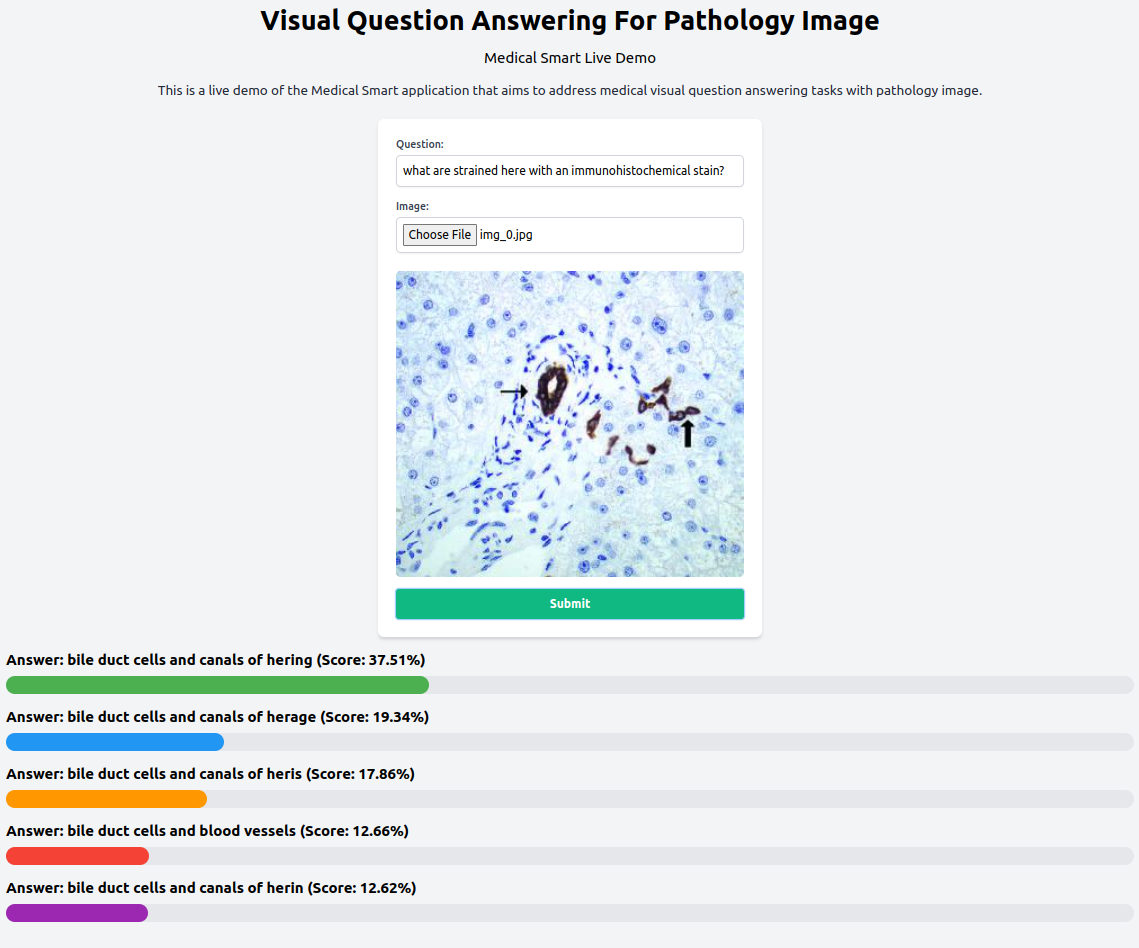
\includegraphics[width=\textwidth, height=10cm]{image/lampiran/patologi-1.png}
  \end{figure}

  \begin{figure}[H]
    \centering
    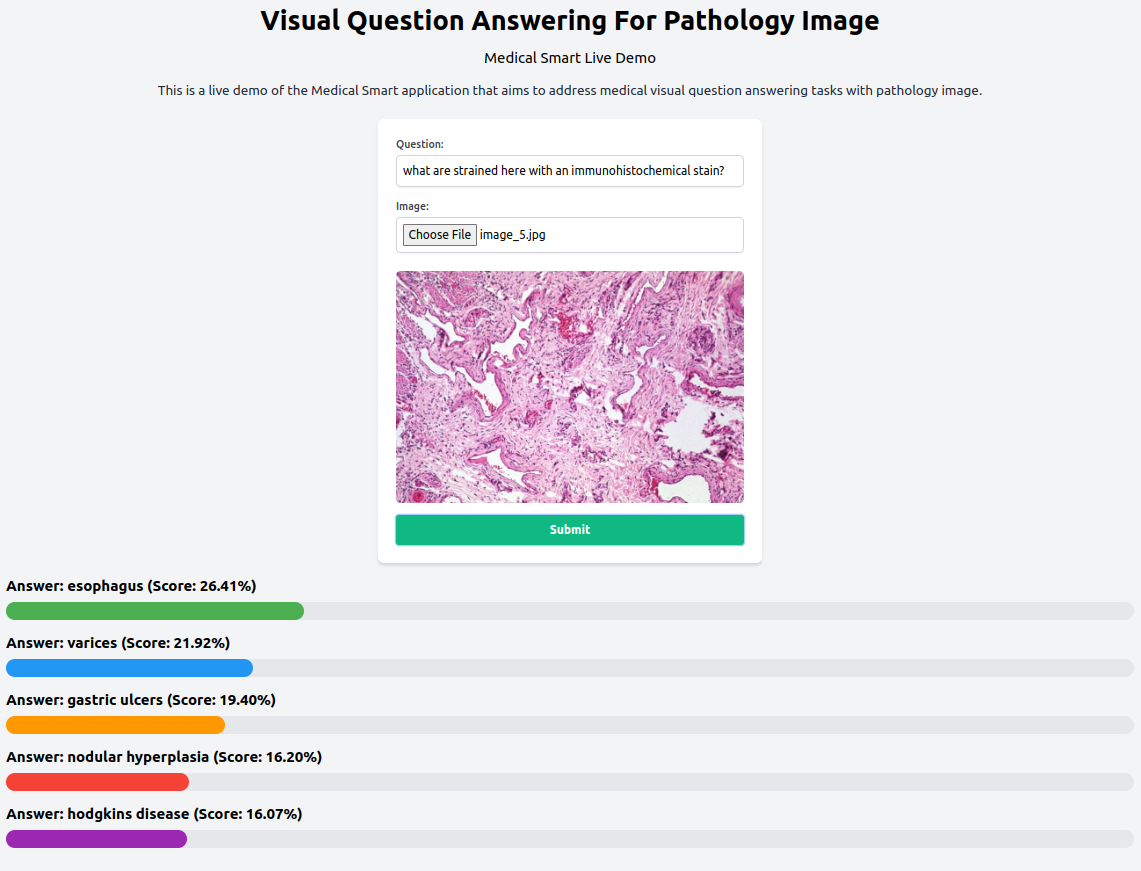
\includegraphics[width=\textwidth, height=10cm]{image/lampiran/patologi-2.png}
  \end{figure}

  \begin{figure}[H]
    \centering
    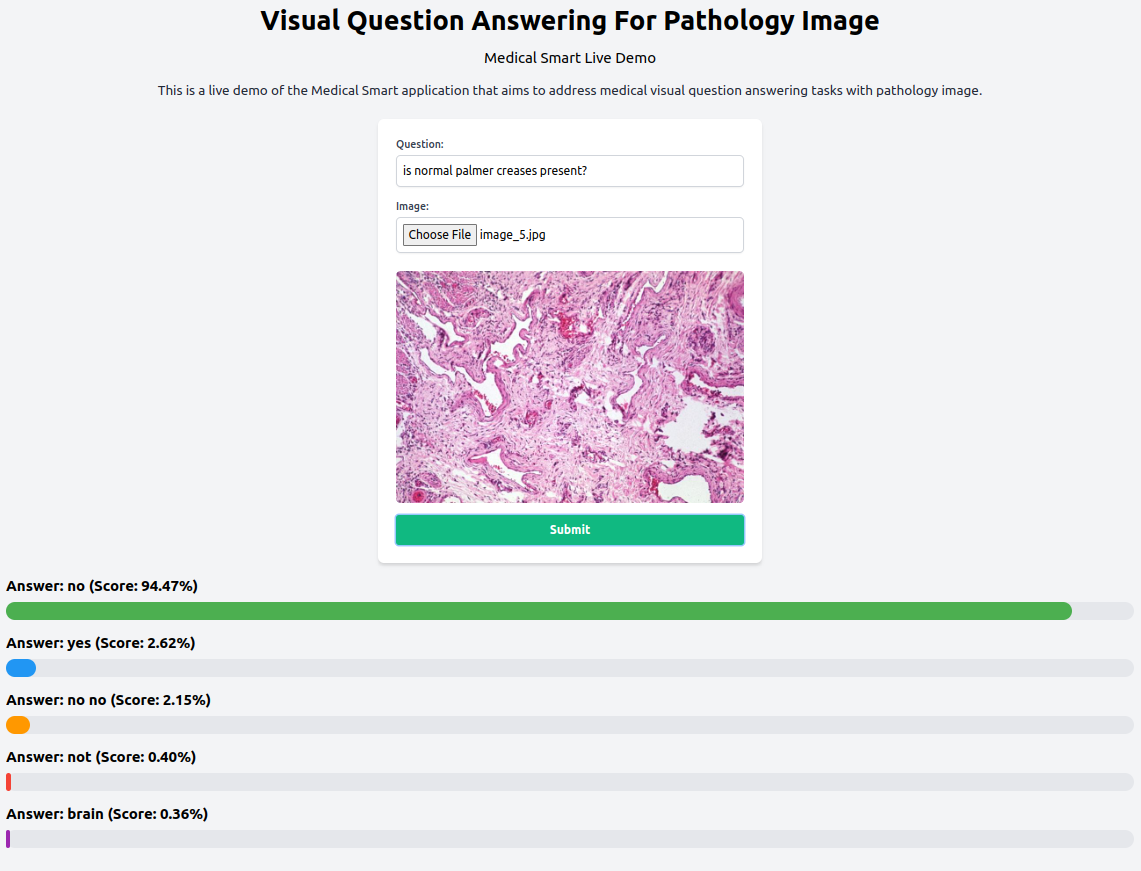
\includegraphics[width=\textwidth, height=11cm]{image/lampiran/patologi-3.png}
  \end{figure}

  \begin{figure}[H]
    \centering
    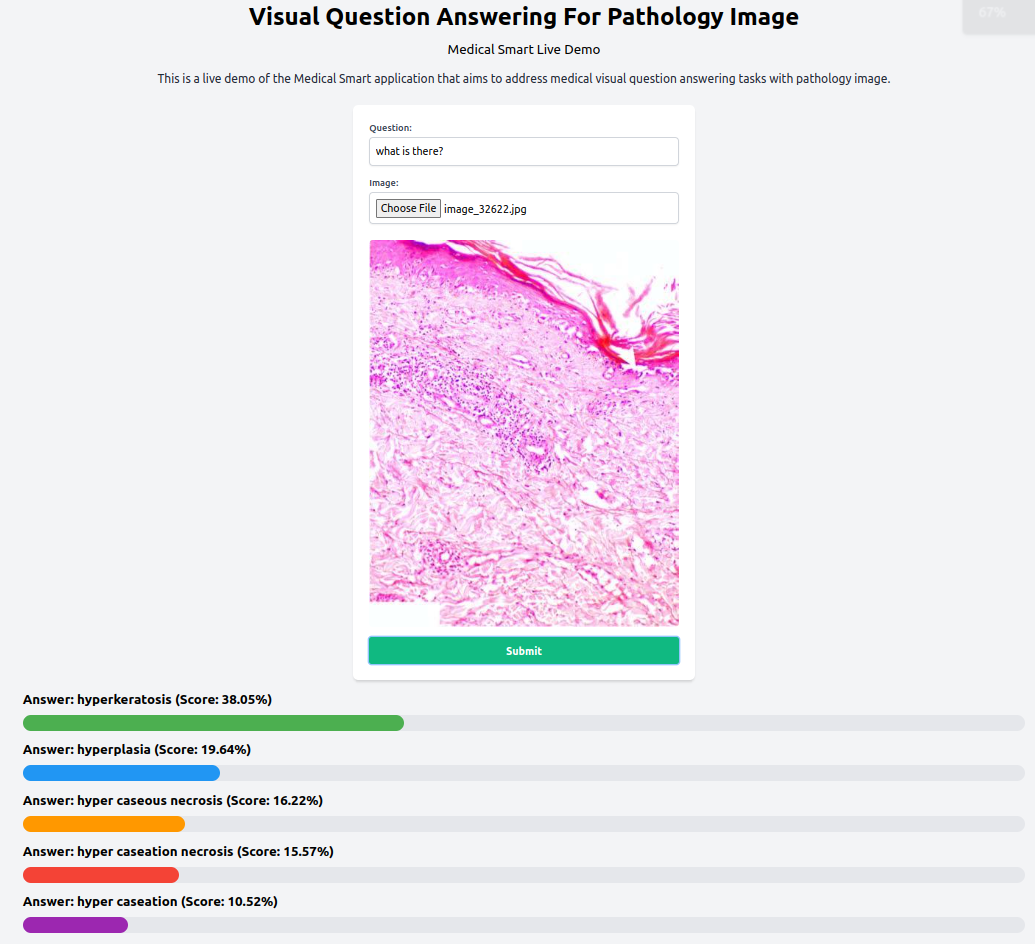
\includegraphics[width=\textwidth, height=10cm]{image/lampiran/patologi-4.png}
  \end{figure}
  

  \newappendix{Lampiran 11. Proses demo pada citra radiologi di halaman web}

  \begin{figure}[H]
    \centering
    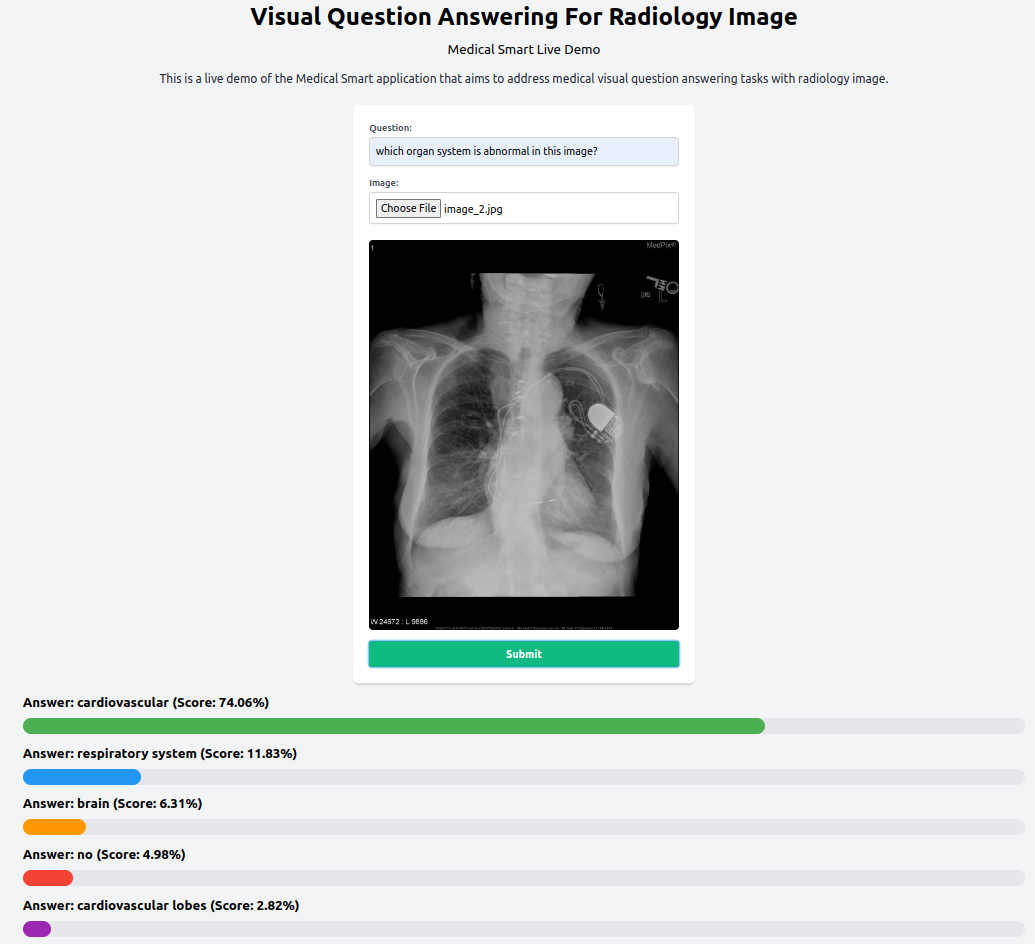
\includegraphics[width=\textwidth, height=10cm]{image/lampiran/radiologi-1.png}
  \end{figure}

  \begin{figure}[H]
    \centering
    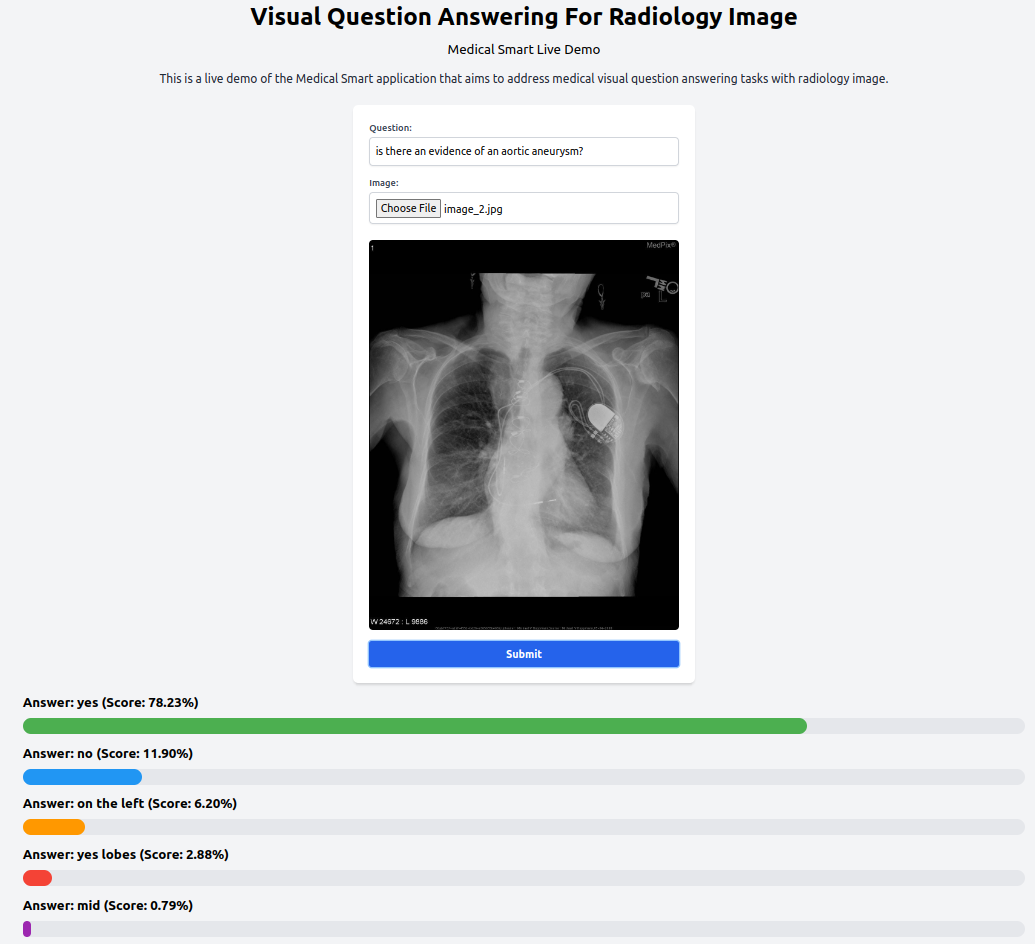
\includegraphics[width=\textwidth, height=11cm]{image/lampiran/radiologi-2.png}
  \end{figure}

  \begin{figure}[H]
    \centering
    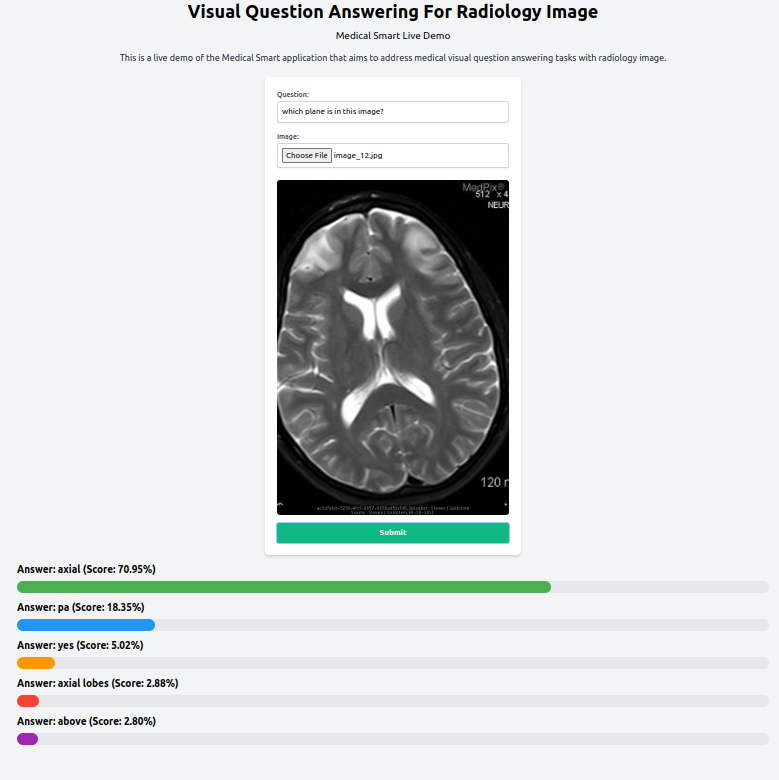
\includegraphics[width=\textwidth, height=11cm]{image/lampiran/radiologi-3.png}
  \end{figure}

  \begin{figure}[H]
    \centering
    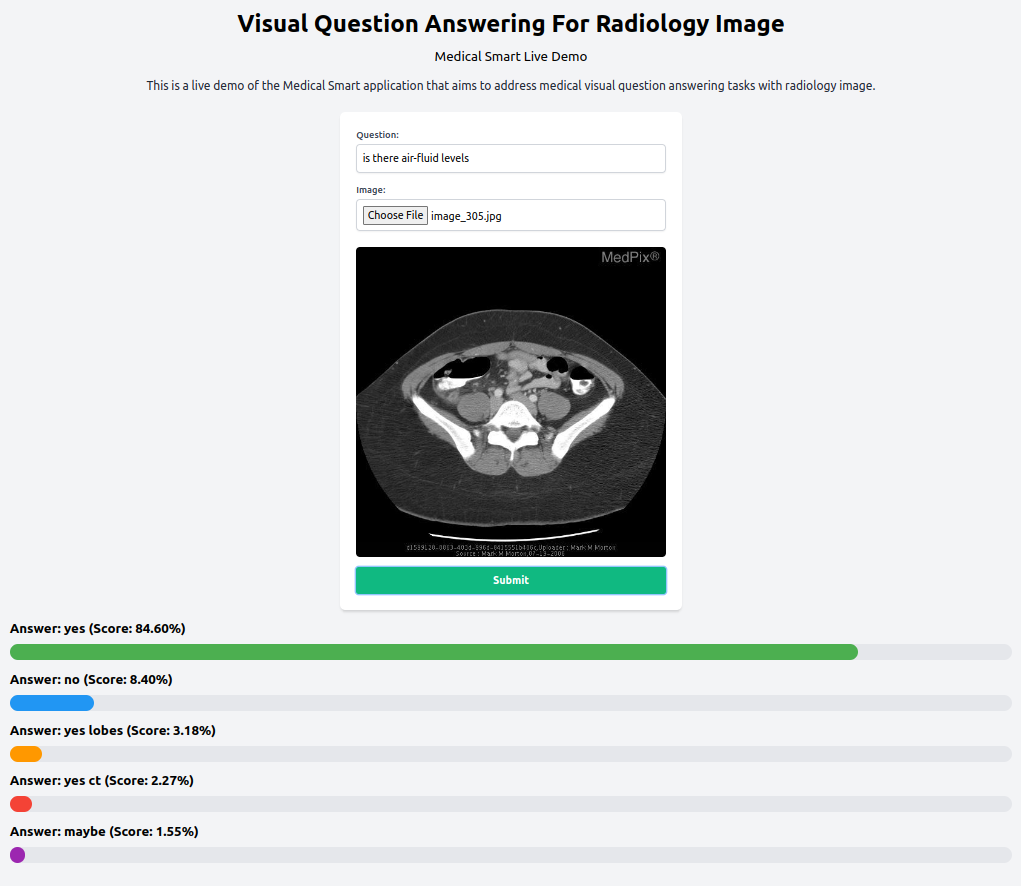
\includegraphics[width=\textwidth, height=11cm]{image/lampiran/radiologi-4.png}
  \end{figure}

  \newappendix{Lampiran 12. Biodata Penulis}

  %\includepdf[pages=-]{tanda-tangan/biodata-signed.pdf} --> Jika sudah ada tanda tangan, komen code bawah dan uncomment code ini

  % space kebawah 1 spasi
  \bigskip
  \vspace{1sp}
  % teks dengan font 14 ke tengah
  \begin{center}
      \fontsize{14}{16}\selectfont
      \textup{\textbf{BIODATA}}
  \end{center}
  % space kebawah 2 spasi
  \vspace{2sp}

  \begin{tabbing}
    \hspace{2in} \= \hspace{2in} \kill
    1. Nama \> : Abdul Hafidh \\
    2. Tempat, tanggal lahir \> : Banda Aceh, 29 Maret 2002 \\
    3. Alamat \> : Jalan Pari No 49 Lampriet Banda Aceh \\
    4. Nama Ayah \> : Fadhli \\
    5. Pekerjaan Ayah \> : Swasta \\
    6. Nama Ibu \> : Dewi Ratna Sari \\
    7. Pekerjaan Ibu \> : Pegawai Negeri Sipil \\
    8. Alamat Orang Tua \> : Jalan Pari No 49 Lampriet Banda Aceh \\
    9. Riwayat Pendidikan \> : 
  \end{tabbing}

  \begin{table}[H]
  \centering
  \resizebox{\textwidth}{!}{%
  \begin{tabular}{|c|c|c|c|c|}
  \hline
  \multicolumn{1}{|l|}{Jenjang} & \multicolumn{1}{l|}{Nama Sekolah} & \multicolumn{1}{l|}{Bidang Studi} & \multicolumn{1}{l|}{Tempat} & \multicolumn{1}{l|}{Tahun Ijazah} \\ \hline
  SD  & SD Kartika XIV-1 Banda Aceh     & -   & Banda Aceh & 2014 \\ \hline
  SMP & SMP Fatih Bilingual School Banda Aceh & -   & Banda Aceh & 2017 \\ \hline
  SMA & SMA Fatih Bilingual School Banda Aceh & IPA & Banda Aceh & 2020 \\ \hline
  \end{tabular}%
  }
  \end{table}


  \begin{tabular}{p{7.5cm}l}
    &Banda Aceh, 8 Juli 2024\\
    &\\
    &\\
    &\multirow{1.5}{7.5cm}{\underline{Abdul Hafidh}} \\ 
    &NPM. 2008107010056 \\
  \end{tabular}

      
\addcontentsline{toc}{chapter}{LAMPIRAN} %daftar lampiran

\end{onehalfspace}

\end{document}